\documentclass[fleqn,11pt]{report}

\usepackage[utf8]{inputenc}
%\usepackage[russian]{babel}
\usepackage{xypic}
\usepackage{subcaption}
\usepackage{textcomp}
\usepackage{booktabs} % For formal tables
\usepackage{amsmath}
\usepackage{semantic}
\usepackage{natbib}
\usepackage{amssymb}
\usepackage{amsthm}
\usepackage[usenames,dvipsnames]{xcolor}
\usepackage{graphicx}
\usepackage{endnotes}
\usepackage{sectsty}
\usepackage[a4paper, margin=1.4in]{geometry}
\usepackage[hang,flushmargin]{footmisc}
\usepackage[font=small,labelfont=bf]{caption}
% \usepackage{tgtermes}
\usepackage[sfdefault,lf]{carlito}
%\usepackage{lmodern}
%\usepackage[scaled]{beramono}
\usepackage[scaled=0.8]{noto}
\usepackage[T1]{fontenc}
\usepackage{bibentry}

% \usepackage{caladea}
\usepackage[colorlinks]{hyperref} % [hidelinks]
\usepackage{hypcap}
\usepackage{listings}
\usepackage{stmaryrd}
\usepackage{enumerate}

\newcommand{\Din}{X}
\newcommand{\Dout}{Y}
\DeclareMathOperator{\choices}{\mathit{choices}}
\DeclareMathOperator{\best}{\mathit{best}}
\DeclareMathOperator{\argmax}{\mathrm{arg\,max}}

\newcommand{\lsep}[0]{\;\; | \;\;}
\newcommand{\kvd}[1]{\textnormal{\ttfamily\bfseries #1}}
\newcommand{\ident}[1]{\textnormal{\ttfamily #1}}
\newcommand{\qident}[1]{\textnormal{\ttfamily '#1'}}

\definecolor{kvdclr}{rgb}{0.0,0.0,0.6}
\definecolor{numclr}{rgb}{0.0,0.4,0.0}
\definecolor{prepclr}{rgb}{0.6,0.0,0.2}
\newcommand{\Num}[1]{\textcolor{numclr}{#1}}
\newcommand{\bndclr}[1]{\textcolor{kvdclr}{#1}}
\newcommand{\bkndclr}[1]{\textcolor{prepclr}{#1}}
\newcommand{\blblclr}[1]{\textcolor{numclr}{#1}}
\newcommand{\bnd}[1]{\textnormal{\textcolor{kvdclr}{\sffamily #1}}}
\newcommand{\bknd}[1]{\textnormal{\textcolor{prepclr}{\sffamily #1}}}
\newcommand{\blbl}[1]{\textnormal{\textcolor{numclr}{\sffamily #1}}}
\newcommand{\narrow}[1]{\hspace{-0.6em}#1\hspace{-0.6em}}

\newcommand{\langl}{\begin{picture}(4.5,7)
\put(1.1,2.5){\rotatebox{60}{\line(1,0){5.5}}}
\put(1.1,2.5){\rotatebox{300}{\line(1,0){5.5}}}
\end{picture}}
\newcommand{\rangl}{\begin{picture}(4.5,7)
\put(.9,2.5){\rotatebox{120}{\line(1,0){5.5}}}
\put(.9,2.5){\rotatebox{240}{\line(1,0){5.5}}}
\end{picture}}
\newcommand{\vect}[1]{\langl #1 \rangl}

%\theoremstyle{definition}
\newtheorem{theorem}{Theorem}
\theoremstyle{definition}
\newtheorem{definition}{Definition}

\newcommand{\tytagof}{\ident{tagof}}
\newcommand{\reduce}{\rightsquigarrow}
\newcommand{\sem}[1]{\llbracket #1 \rrbracket}
\newcommand{\semalt}[1]{S(#1)}

\newenvironment{nitemize}
{ \vspace{-0.4em}
  \begin{itemize}
    \setlength{\itemsep}{5pt}
    \setlength{\parskip}{0pt}
    \setlength{\parsep}{0pt} }
{ \end{itemize}
  \vspace{-0.4em} }

\newenvironment{nenumerate}
{ \vspace{-0.4em}
  \begin{enumerate}
    \setlength{\itemsep}{5pt}
    \setlength{\parskip}{0pt}
    \setlength{\parsep}{0pt} }
{ \end{enumerate}
  \vspace{-0.4em} }


\hypersetup{
linkcolor=Black,
citecolor=Mahogany,
filecolor=Black,
urlcolor=Blue,
menucolor=Black,
runcolor=Black
}
\renewcommand\enoteformat{%
  \raggedright
  \leftskip=1.8em
  \makebox[0pt][r]{\theenmark. \rule{0pt}{\dimexpr\ht\strutbox+}}%
}

\lstdefinestyle{mystyle}{
  commentstyle=\color{ForestGreen},
  keywordstyle=\color{NavyBlue},
  ndkeywordstyle=\color{Fuchsia},
  stringstyle=\color{Maroon},
  basicstyle=\ttfamily,
  numbers=left,
  numberstyle=\footnotesize,
  xleftmargin=3em
}

\lstdefinelanguage{thegamma}{
  keywords={let},
  morecomment=[l]{//},
  morecomment=[s]{/*}{*/},
  morestring=[b]",
  sensitive=true
}
\lstdefinelanguage{fluid}{
  keywords={let,fun},
  ndkeywords={BarChart,LineChart,LinePlot},
  morestring=[b]",
  sensitive=true
}
\lstdefinelanguage{sharp}{
  keywords={var,in,foreach,let,type,null,match,with,for,do},
  ndkeywords={fill,cat,cont,padding,axis,overlay,rect},
  morecomment=[l]{//},
  morecomment=[s]{/*}{*/},
  morestring=[b]",
  sensitive=true
}
\lstdefinelanguage{ppython}{
  keywords={False},
  morecomment=[l]{//},
  morecomment=[s]{/*}{*/},
  morestring=[b]",
  sensitive=true
}
\lstset{style=mystyle}

\urlstyle{sf}

\widowpenalties 2 10000 0
\sectionfont{\large}
\chaptertitlefont{\LARGE}
%\renewcommand*\thesection{\arabic{section}}
%\setcounter{secnumdepth}{0} % sections are level 1


\begin{document}
\title{\Huge\textbf{Simple programming tools \\for data exploration}}
\author{Tomas Petricek}
\maketitle

\chapter*{Preface}
\label{ch:preface}
\addcontentsline{toc}{chapter}{\nameref{ch:preface}}

This thesis presents a selection of my recent research that focuses on making programming
tools for data exploration simpler. The origins of this research direction can be traced to
my involvement with the F\# programming language. When Don Syme and the F\# team at Microsoft
developed the first versions of the F\# type provider mechanism, I started my first experiments
that eventually led to the type providers for structured data presented as one of the contributions
in this thesis. However, seeing how easy working with data in a programming language can be
led me to a further question: Could we make programmatic data exploration easy enough that it
could be done by non-programmers? The rising popularity of data journalism at the time provided
a further practical motivation.

The work presented in this thesis has been done at a number of institutions, starting towards the
end of my PhD at University of Cambridge and finishing as I was joining the Department of
Distributed and Dependable Systems (D3S) at the Faculty of Mathematics and Physics. In between,
I spent time at Microsoft Research in Cambrige, The Alan Turing Institute in London and the
University of Kent in Canterbury. I am grateful to all those institutions for enabling me to
pursue my research vision.

Although I am the first author of most of the work presented in this thesis, none of it would be
possible without the many collaborators that I was fortunate to meet along the way. Don Syme
not only provided the initial motivation and collaborated with me on multiple papers, but also
became my long-term mentor and a friend. The work related to F\# received warm welcome from the
friendly F\# community and early commercial adopters. Gustavo Guerra deserves a special credit
for turning F\# Data from a prototype to a well-engineered (and widely adopted) package.

At The Alan Turing Institute, I was fortunate to meet James Geddes who got me involved in the
AI for Data Analytics (AIDA) project. The bridging of different worlds that James made possible
resulted in my involvement in research on notebooks and data provenance with Charles Sutton,
but also work on automating data wrangling with Gerrit van den Burg, Alfredo Nazábal, Taha Ceritli,
Ernesto Jim\'enez-Ruiz and Chris William. The Alan Turing Institute also provided initial funding
for our joint work on data visualization tools with Roly Perera.

In addition to direct collaborators, the work presented in this thesis benefited from numerous
discussions with my other colleagues and friends. This includes Dominic Orchard and Stephen Kell
first at University of Cambridge and then at University of Kent,
Kenji Takeda, Jomo Fisher and Keith Battocchi at Microsoft Research
and May Yong, Nick Barlow, Brooks Paige at The Alan Turing Institute.
Mathias Brandewinder, Jonathan Edwards, Nour Boulahcen, Luke Church, Clemens Klokmose,
Mariana Marasoiu and Alan Blackwell also provided ideas, insights, technical contributions
and valuable feedback on some of the works presented as part of this thesis.

~

The work presented in this thesis also received valuable support from industrial collaborators.
My research focused on data journalism benefited from discussions with
Megan Lucero from The Bureau of Investigative Journalism. My work on F\# was supported by
the wide and enthusiastic F\# community and also by Howard Mansell and BlueMountain Capital.
I had the pleasure of presenting many of the ideas at a number of industry conferences,
including NDC in Oslo and London, LambdaDays and DevDay in Krak\'ow, GOTO in Copenhagen and Chicago,
CogX London and, most recently, the F\# Data Science conference in Berlin. These presentations
were vital not only for enabling industry adoption of some of the systems presented in this thesis,
but also provided valuable feedback.

Over time, the work has been financially supported in a number of ways. The Google Digital News
Initiative provided me with a generous individual grant that allowed me to fully focus on
programming tools for data journalism for one and half years. Microsoft Research,
BlueMountain Capital, University of Kent and Charles University paid for some of my time over
the years. At The Alan Turing Institute, I was supported by The UKRI Strategic Priorities Fund
under EPSRC Grant EP/T001569/1, particularly the Tools, Practices and Systems theme within that
grant, through the UK Government's Defence & Security Programme and by The Alan Turing Institute
under EPSRC grant EP/N510129/1. At Charles University, I was a part of the
Department of Distributed and Dependable Systems and I was also supported by the PRIMUS
grant PRIMUS/24/SCI/021.

\addcontentsline{toc}{chapter}{Contents}
\tableofcontents

\part{Commentary}

% ==================================================================================================
% CHAPTER 1: INTRODUCTION
% ==================================================================================================

\chapter{Introduction}

The rise of big data, open government data initiatives \citep{attard-2015-opengov},\footnote{See
\url{https://data.gov} and \url{https://data.gov.uk}, but also \url{https://opendata.gov.cz} as
examples.} and civic data initiatives mean that there is an increasing amount of raw data available
that can be used to understand the world we live in, while increasingly powerful machine learning
algorithms give us a way to gain insights from such data. At the same time, the general
public increasingly distrusts statistics \citep{davies-2017-statistics} and the belief that we
live in a post-truth era has become widely accepted over the last decade.

While there are complex socio-political reasons for this paradox, from a merely technical
perspective, the limited engagement with data-driven insights should perhaps
not be a surprise. We lack accessible data exploration technologies that would allow
non-programmers such as data journalists, public servants and analysts to produce transparent data
analyses that can be understood, explored and adapted by a broad range of end-users including
educators, the public and the members of the civic society.

The technology gap is illustrated in Figure~\ref{fig:gap}. On the one hand, graphical tools such as
spreadsheets are easy to use, but they are limited to small tabular data sets, they are error-prone
\citep{panko-2015-errors} and they do not aid transparency. On the other hand, programmatic tools for
data exploration such as Python and R can tackle complex problems, but require expert programming
skills for completing even the simplest tasks.

\begin{figure}[h!]
\centering
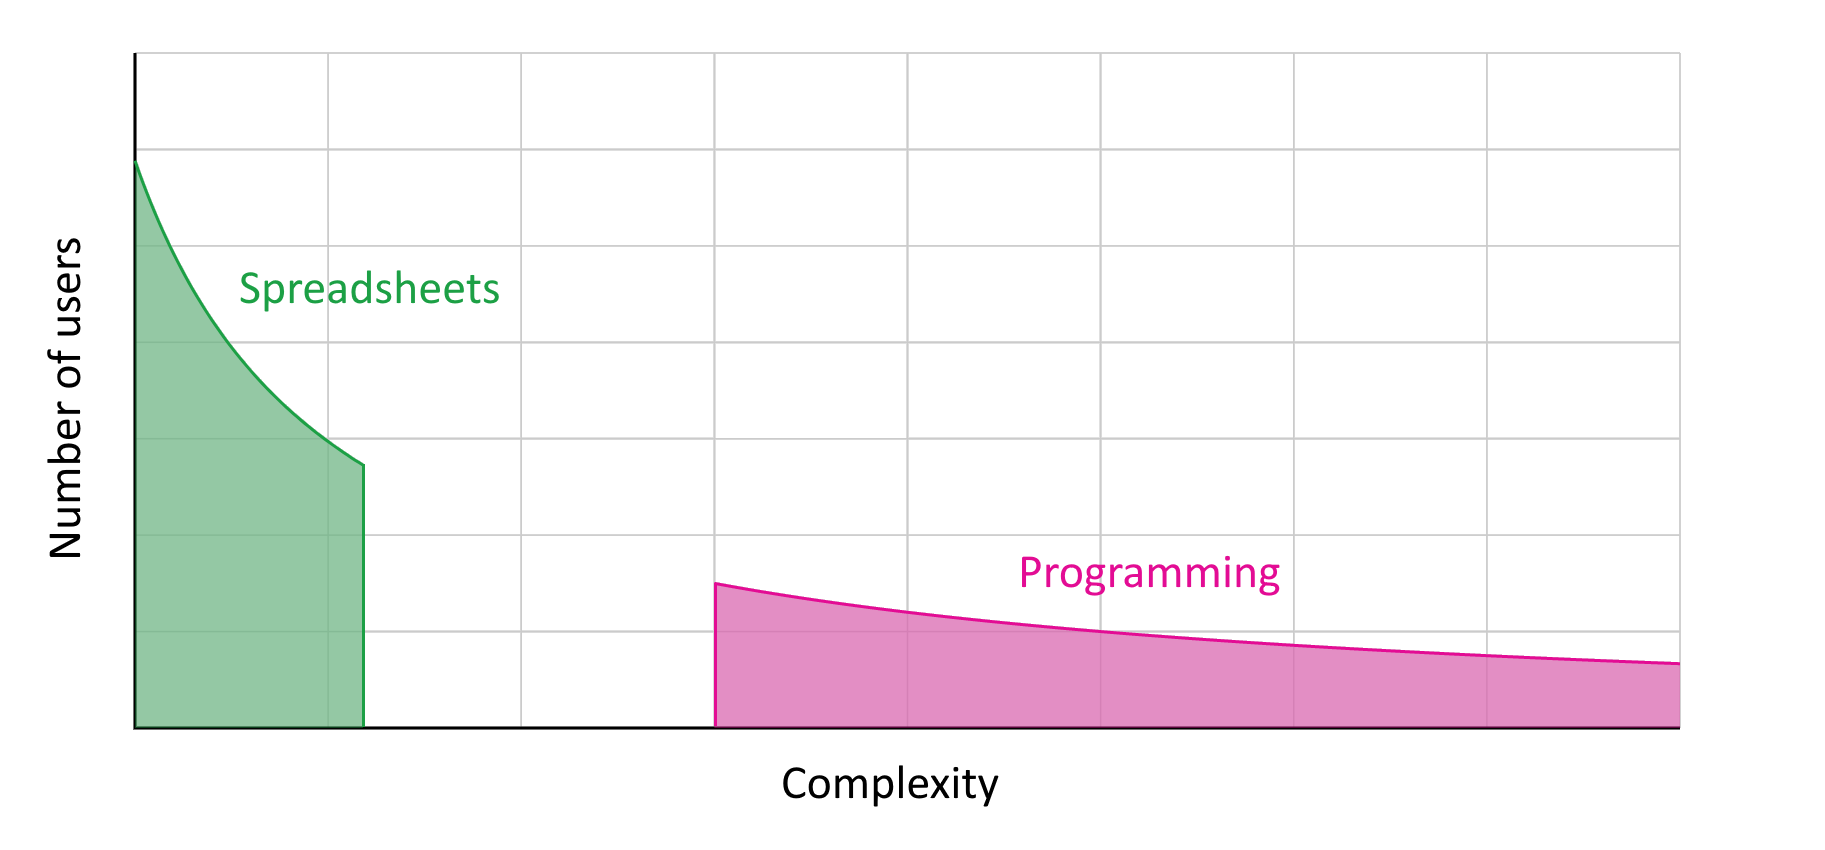
\includegraphics[scale=0.25]{img/gap.png}
\vspace{-0.5em}
\caption{The gap between programming and spreadsheets -- spreadsheets can be used by many people,
but solve problems of a limited complexity. Programming scales arbitrarily, but has a high minimal
complexity limiting the number of users. Adapted from \citet{edwards-2015-transcript}.}
\label{fig:gap}
\end{figure}

The above illustration should not be taken at face value. Although there is no single accepted
solution, there are multiple projects that exist in the gap between spreadsheets and programming
tools. However, the gap provides a useful perspective for positioning the contributions presented
in this thesis. Some of the work develops novel tools that aim to combine the simplicity of
spreadsheets with the power of programming for the specific domain of data exploration, aiming to
fill the space in the middle of the gap. Some of the work I present focuses on making regular
programming with data easier, or making simple programming with data accessible to a greater
number of users, reducing the size of the gap on the side of programming.

\begin{figure}[t]
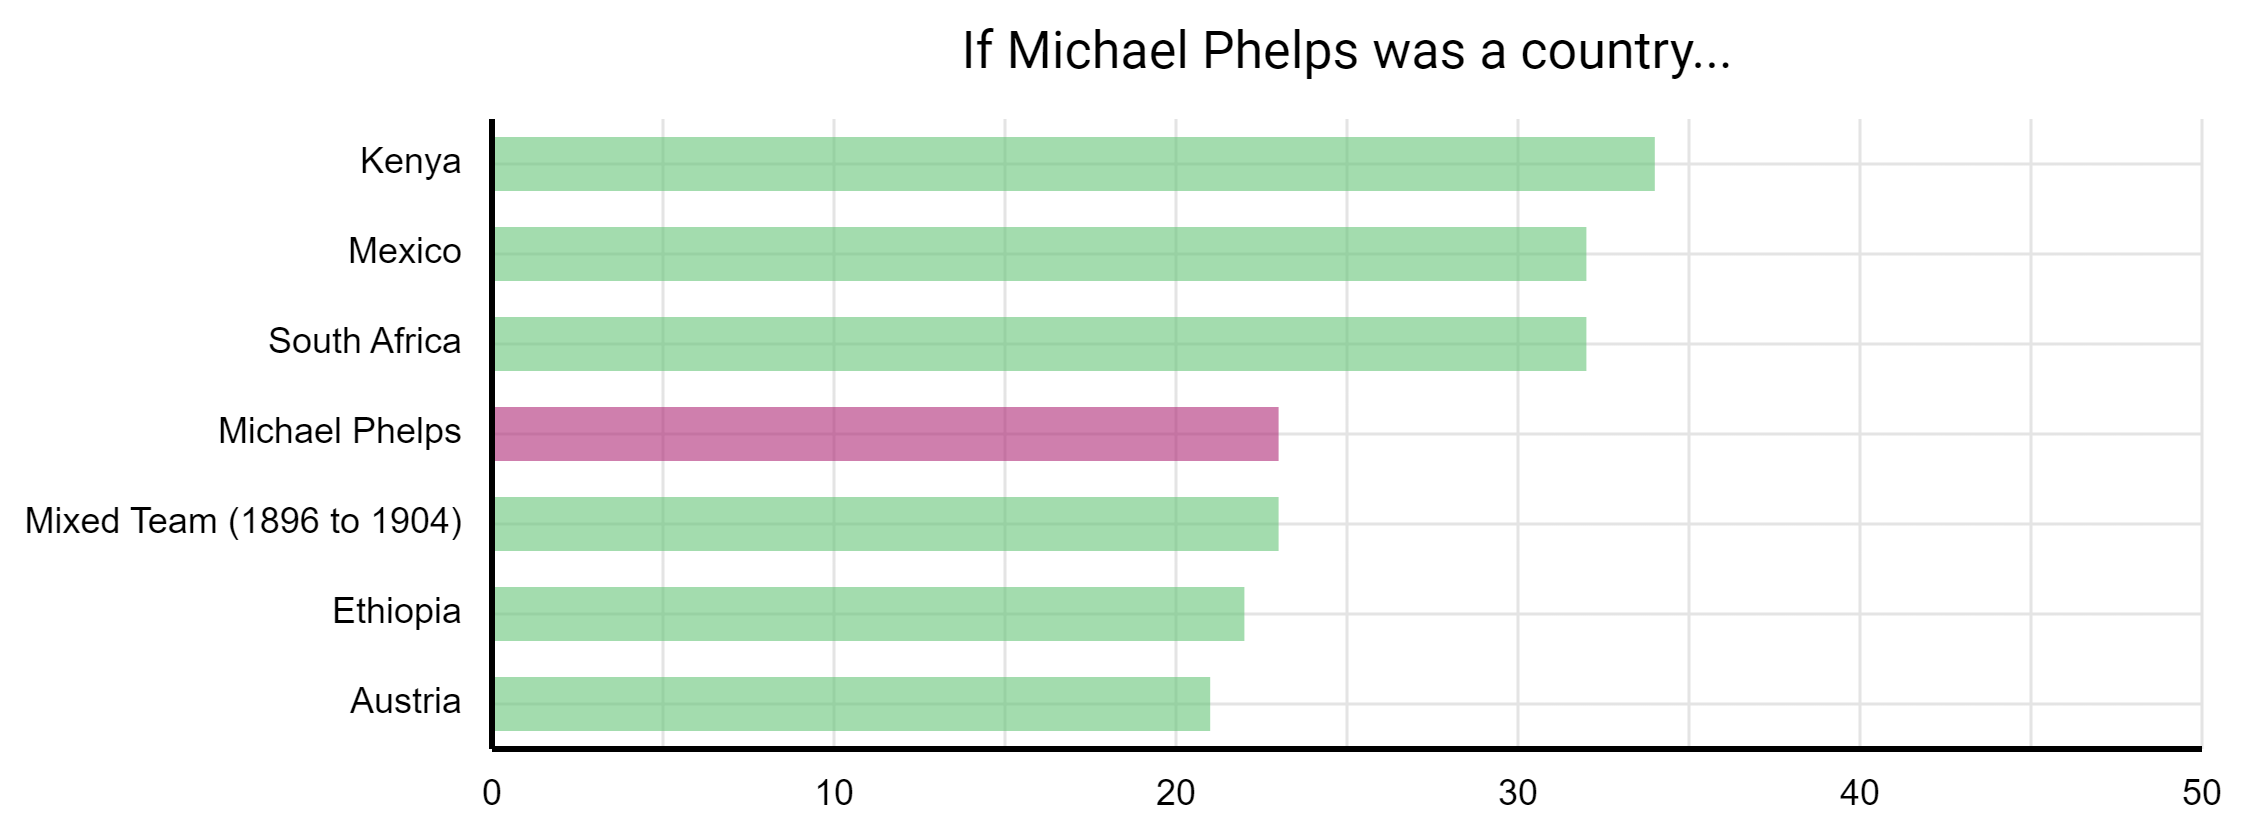
\includegraphics[scale=0.345]{img/phelps.png}
\caption{A visualization comparing the number of gold Olympic medals won by Michael Phelps
 with countries that won a close number of gold medals. Inspired by e.g., \cite{npr-2016-phelps}}
\label{fig:phelps}
\end{figure}

\section{How data journalists explore data}
\label{sec:intro-ddj}

To explain the motivation of this thesis, I use an example data exploration done in the context of
data journalism \citep{bounegru-2021-handbook}. Following the phenomenal success of the swimmer
Michael Phelps at the 2016 Olympic games, many journalists produced charts such as the one
in Figrue~\ref{fig:phelps}, which puts Phelps on a chart showing countries with similar number
of medals. Even such simple visualization raises multiple questions. Is the table counting
Gold medals or all medals? Would it change if we used the other metric? What would it look like
if we added more countries or removed the historical ``Mixed Team''? How many top countries
were skipped?

This simple example illustrates two challenges that I hinted at earlier. First, producing this
visualization may not be hard for a programmer, but it involves a number of tricky problems
for a non-programmer. It has to acquire and and clean the source data, aggregate medals by
country and produce and join two subsets of the data. Doing so manually in a spreadsheet
is tedious, error-prone and not reproducible, but using Python or R requires non-trivial programming
skills. Second, the non-technical reader of the newspaper article may want to answer the above
follow-up questions. Data journalists sometimes offer download of the original dataset, but the
reader would then have to redo the analysis from scratch. If the data analysis was done in Python
or R, they could get the source code, but this would likely be too complex to modify.

This thesis presents a range of tools that allow non-programmers, such as data journalists, to
clean and explore data, such as the table of Olympic medals, and produce data analyses that are
backed by source code in a simple language that can be read and understood without sophisticated
programming skills. The code can be produced interactively, by repeatedly choosing one from a
range of options offered by the tool and can then be modified to change parameters of the
visualization.

\begin{figure}[t]
\begin{lstlisting}[language=thegamma]
let data = olympics.'group data'.'by Team'.'sum Gold'.then
    .'sort data'.'by Gold descending'.then
    .paging.skip(42).take(6)
    .'get series'.'with key Team'.'and value Gold'

let phelps = olympics.'filter data'.'Athlete is'.'Michael Phelps'.then
    .'group data'.'by Athlete'.'sum Gold'.then
    .'get series'.'with key Athlete'.'and value Gold'

charts.bar(data.append(phelps).sortValues(true))
    .setColors(["#94c8a4","#94c8a4","#94c8a4","#e30c94"])
\end{lstlisting}
\caption{Source code of the data analysis used to produce the visualization in
Figure~\ref{fig:phelps}. The case study is based on the work presented in Chapter~\ref{ch:thegamma}.}
\label{fig:gamma}
\end{figure}

As an example, the source code of the data analysis used to produce the visualization above is shown
in Figure~\ref{fig:gamma}. The tools that enable non-programmers to create it will be discussed
later. The key aspect of the code is that it mostly consists of sequence of human-readable
commands such as \ident{'filter data'.'Athlete is'.'Michael Phelps'}. Those are iteratively
selected from options offered by the system and so the author of the data analysis can complete
most of the analysis without writing code.

The use of a simple programming language also makes it possible to understand the key
aspects of the logic. The analysis counts the number of gold medals (\ident{'sum Gold'}),
skips 42 countries before the ones shown in the visualization and does not filter out any
other data. Finally, the code can be easily executed (in a web browser), allowing the reader
to easily make small changes, such as pick a different athlete or increase the number of displayed
countries. Such engagement has the potential to aid their positive percpetion of open, transparent
data-driven insights based on facts.

\section{Requirements of simple tools for data exploration}

Although the tools and techniques presented in this thesis are more broadly applicable,
the focus of this thesis is on a narrower domain illustrated by the above motivating example.
I focus on programmatic data exploration tools that can be used to produce accessible and
transparent data analyses that will be of interest to a broader range of readers and allow
them to critically engage with the data.

In the subsequent discussion, I thus distinguish between \emph{data analysts} who produce the
analyses and \emph{readers} who consume and engage with the results. The former are
technically-skilled and data-literate, but may not have programming skills. The latter are
non-technical domain experts who may nevertheless be interested
in understanding and checking the analysis or modifying some of its attributes.
This context leads to a number of requirements for the envisioned data exploration tools:

~

\begin{nitemize}
\item \emph{Gradual progression from simple to complex}. The system must allow non-program\-mers with
limited resources to easily complete simple tasks in an interface that allows them to later
learn more and tackle harder problems. In the technical dimensions of programming systems
framework \citep{jakubovic-2023-techdims}, this is described as the staged levels of complexity
approach to the learnability dimension.

\item \emph{Support transparency and openness}. The readers of the resulting data analyses must
be able to understand how the analysis was done and question what processing steps and parameters
have been used in order to critically engage with the problem.

\item \emph{Enable reproduction and learning by percolation}. A reader should be able to see and
redo the steps through which a data exploration was conducted. This lets them reproduce the results,
but also learn how to use the system. As noted by \citet{sarkar-2018-spreadsheets}, this is how
many users learn the spreadsheet formula language.

\item \emph{Encourage meaningful reader interaction}. The reader should not be just a passive
consumer of the data analyses. They should be able to study the analysis, but
also make simple modifications such as changing analysis or visualization parameters,
as is often done in interactive visualizations by journalists \citep{kennedy-2021-engagements}.
\end{nitemize}

The above criteria point at the gap between spreadsheets and regular programming systems
illustrated by Figure~\ref{fig:gap} and there are multiple possible solutions and approaches to
satisfy the above criteria. This thesis explores one particular point in the design space,
which is to treat data analysis as a program with an open source code, created in a simple
programming language with rich tooling.

As I will show, treating data exploration as a programming problem makes it possible to satisfy
the above criteria. Gradual progression from simple to complex can be supported by a language
that provides very high-level abstractions (or domain-specific langauges) for solving simple
problems. Transparency, openness and reproducibility are enabled by the fact that the source code
is always available and can be immediately executed, while learning
by percolation can be supported by structuring the program as a sequence of transformations.
Finally, meaningful interaction can be offered by suitable graphical tools that simpify editing
of the underlying source code.

\section{Data exploration as a programming problem}

Data exploration is typically done using a combination of tools including spreadsheets,
programming tools, online systems and ad-hoc utilities. Spreadsheets like Excel and business
intelligence tools like Tableau \citep{wesley-2011-tableau} are often used for manual data
editing, reshaping and visualization. More complex and automated data analyses are done in
programming languages like R and Python using a range of data processing libraries such as pandas
and Tidyverse \citep{wickham-2019-tidyverse}. Such analyses are frequently done in a computational
notebook environments such as RStudio or Jupyter \citep{kluyver-2016-jupyter}, which make
it possible to interleave documentation, mathematical formulas and code with outputs such as
visualizations. Online data processing environments like Trifacta provide myriads of tools for
importing and transforming data, which are accessible through different user interfaces or
programmatic interfaces, but even those have to be complemented with ad-hoc single-purpose tools,
often invoked through a command line interface.

Finding a unified perspective for thinking about such hotchpotch of systems and tools
is a challenge. The view taken in this thesis is that, most of the systems and tools can be
considered as programming systems. This view makes it possible to apply the powerful methodology
of programming languages research to the problem of data exploration.
However, the programs that are constructed during data exploration have a number of specific
characteristics that distinguishes them from programs typically considered in programming
langauge research:

\begin{nitemize}
\item \emph{Data exists alongside code}. Systems such as spreadsheets often mix
  data and code in a single environment. In conventional programming, this is done in
  image-based systems like Smalltalk, but not in the context of programming languages.

\item \emph{Concrete inputs are often known}. Moreover, data exploration is typically done on a
  known collection of concrete input datasets. This means that program analysis can take
  this data into account rather than assuming arbitrary unknown inputs.

\item \emph{Programmers introduce fewer abstractions}. Even in programmatic data exploration using
  R or Python in a Jupyter notebook, data analysts often write code as a sequence of
  direct operations on inputs or previously computed results, rather than introducing abstractions
  such as reusable generic functions.

\item \emph{Most libraries are externally defined}. Finally, data exploration is
  often done using libraries and tools that are implemented outside of the tool that the analysts
  use. For example, spreadsheet formulas use mostly built-in functions, while data analyses in
  Python often use libraries implemented in C/C++ for performance reasons.
\end{nitemize}

The above generally hold for simple data explorations that are done by data journalists, public
servants and analysts that this thesis is primarily concerned with. The characteristics do not
apply to all programs that work with data, which may include complex reusable and parameterized
models, general-purpose algorithms and rich data processing pipelines. However, focusing on simple
data exploration problems for which the above criteria are true allows us to narrow the design
space and study a range of interesting problems. The narrow focus also makes us rethink a number of
accepted assumptions in programming language research, such as what are the key primitives to be
included in a formal model of a programming language (in Chapter~\ref{ch:foundations}, an
invocation of an external function becomes more important than lambda abstraction).

\section{Utilized research methodologies}
The research presented in this thesis tackles multiple research questions such as:
Does a particular language design rule out certain kinds of programming errors? What is an
efficient implementation technique for a particular langauge or a tool? Does a newly
developed tool simplify data exploration by reducing the number of manual interventions
by the user? What is a suitable interaction mechanism for completing a particular task?
And can non-programmers effectively use such interaction mechanism?
The diversity of the research questions calls for a corresponding diversity of research
methodologies.

\paragraph{Programming language theory.}
The first methodology used in this thesis is that of theoretical programming langauge research.
When using this methodology, a core aspect of a programming language is described using a small,
formally tractable mathematical model that captures the essential properties of the aspect.
The model is then used to formally study properties of the given aspect, such as whether a
programming langauge that impements it can be used to write programs that exhibit certain kind
of incorrect behaviour.

In this thesis, Part~\ref{part:providers} presents two instances of a programming language
extension mechanism called type providers. To show that code written using type providers will
never result in a particular error condition, I develop a formal model of type providers and prove
a correctness property using the model. The actual system implementation then closely follows the
formal model. Theoretical programming language research methods are also used to develop a data
visualization laguage in Chapter~\ref{ch:galois}, to formalize the optimization technique introduced
in Chapter~\ref{ch:foundations} and to define the structure of the semi-automatic data wrangling
tools developed in Chapter~\ref{ch:aia}.

\paragraph{Programming systems.}
The theoretical approach is complemented by a range of applied programming systems methods.
The work using those methodologies often focuses on designing suitable system architecture,
empirical evaluation of measurable characteristics of the system such as efficiency. It should
also be complemented with an open-source implementation and/or a reproducibe software artifact.

I use the programming systems research methodology primarily in Chapter~\ref{ch:wrattler}, which
presents the architecture and an implementation of a novel computational notebook system for data
science. Chapter~\ref{ch:foundations} develops an optimized programming assistance tool and
evaluates the efficiency empirically. Software systems and libraries presented in this thesis
are available as open-source and are listed below.

\paragraph{Human-computer interaction.}
Finally, answering questions that concern usability requires a human-centric approach offered by
the human-computer interaction (HCI) research methodology, which is increasingly used to study
programming languages and systems \citep{chasins-2021-plhci}. The HCI methods include controlled
usability studies, qualitative and quantitative user studies, as well as the development and
application of heuristic evaluation frameworks.

I use the HCI methodology in Chapter~\ref{ch:thegamma}, which introduces the ``iterative prompting''
interaction mechanism and conducts a usability study with non-programmers to evaluate whether
they can use it to complete simple data exploration tasks. Chapter~\ref{ch:compost}, which
presents a novel data visualization library, also draws on the HCI methodology, but uses a
comprehensive case study instead of a user study to evaluate the design.

\section{What makes a programming tool simple}

The very title of this thesis refers to the aim of creating programming tools for data exploration
that are \emph{simple}. However, simplicity is difficult to quantify precisely. It is understood
differently by different communitites and in different contexts. I thus follow the recommendation
of \citet{muller-2020-rhetoric} to make explicit how the term should be understood in the
context of this thesis. The notion of simplicity is used as a unifying theme in this commentary.
In the papers presented as part of this thesis, the notion takes one of several more specific and
rigorously evaluated forms:

~

\begin{nitemize}
\item In the context of user-centric work, I refer to a system as \emph{simple} if it allows
  non-programmers to complete tasks that are typically limited to programmers. This is the
  case when discussing the iterative prompting interaction principle in Chapters~\ref{ch:thegamma}
  the live programming tools in Chapter~\ref{ch:foundations}.

\item In the context of programming language or library design, I consider the design \emph{simple}
  when it allows expressing complex logic using a small set of highly composable primitives
  that are easy to understand. This applies to the language design in Chapter~\ref{ch:dotdriven}
  and visualization library design in Chapter~\ref{ch:compost}.

\item In the context of programmer assistance tools, simple indicates that the
  user does not have to perform a task that they would otherwise have to complete manually.
  This applies to AI assistants, presented in Chapter~\ref{ch:aia}, which relieve the user from
  tedious manual setting of parameters by partly automating the task.

\item Finally, I also use the term simple when talking about programming systems and libraries
  that provide a high-level interface designed specifically for a particular task. This is the
  case for the notebook system presented in Chapter~\ref{ch:wrattler}, data access library
  in Chapter~\ref{ch:fsdata} and the language for creating visualizations in Chapter~\ref{ch:galois}.
  Using such high-level abstractions means that programmers have write less code.
\end{nitemize}

The overarching theme of this thesis is thus the design of programming tools for data exploration
that are simple in one or more of the meanings of the term indicated above. The focus on simplicity
aims to fill or reduce the technology gap illustrated in Figure~\ref{fig:gap} and, ultimately,
make data exploration accessible to a broader range of users.

\section{Structure of the thesis contributions}

The contributions of this thesis cover multiple different kinds of tasks that a data analyst
faces when they work with data. To position the contributions in the broader context of data
analytical work, Figure~\ref{fig:lifecycle} shows where they fit in the data science lifecycle
as defined by IBM (with slight modifications). As the diagram shows, the focus of this thesis is on work done in the
initial data exploration phase.

\begin{figure}[h]
  \vspace{1em}
  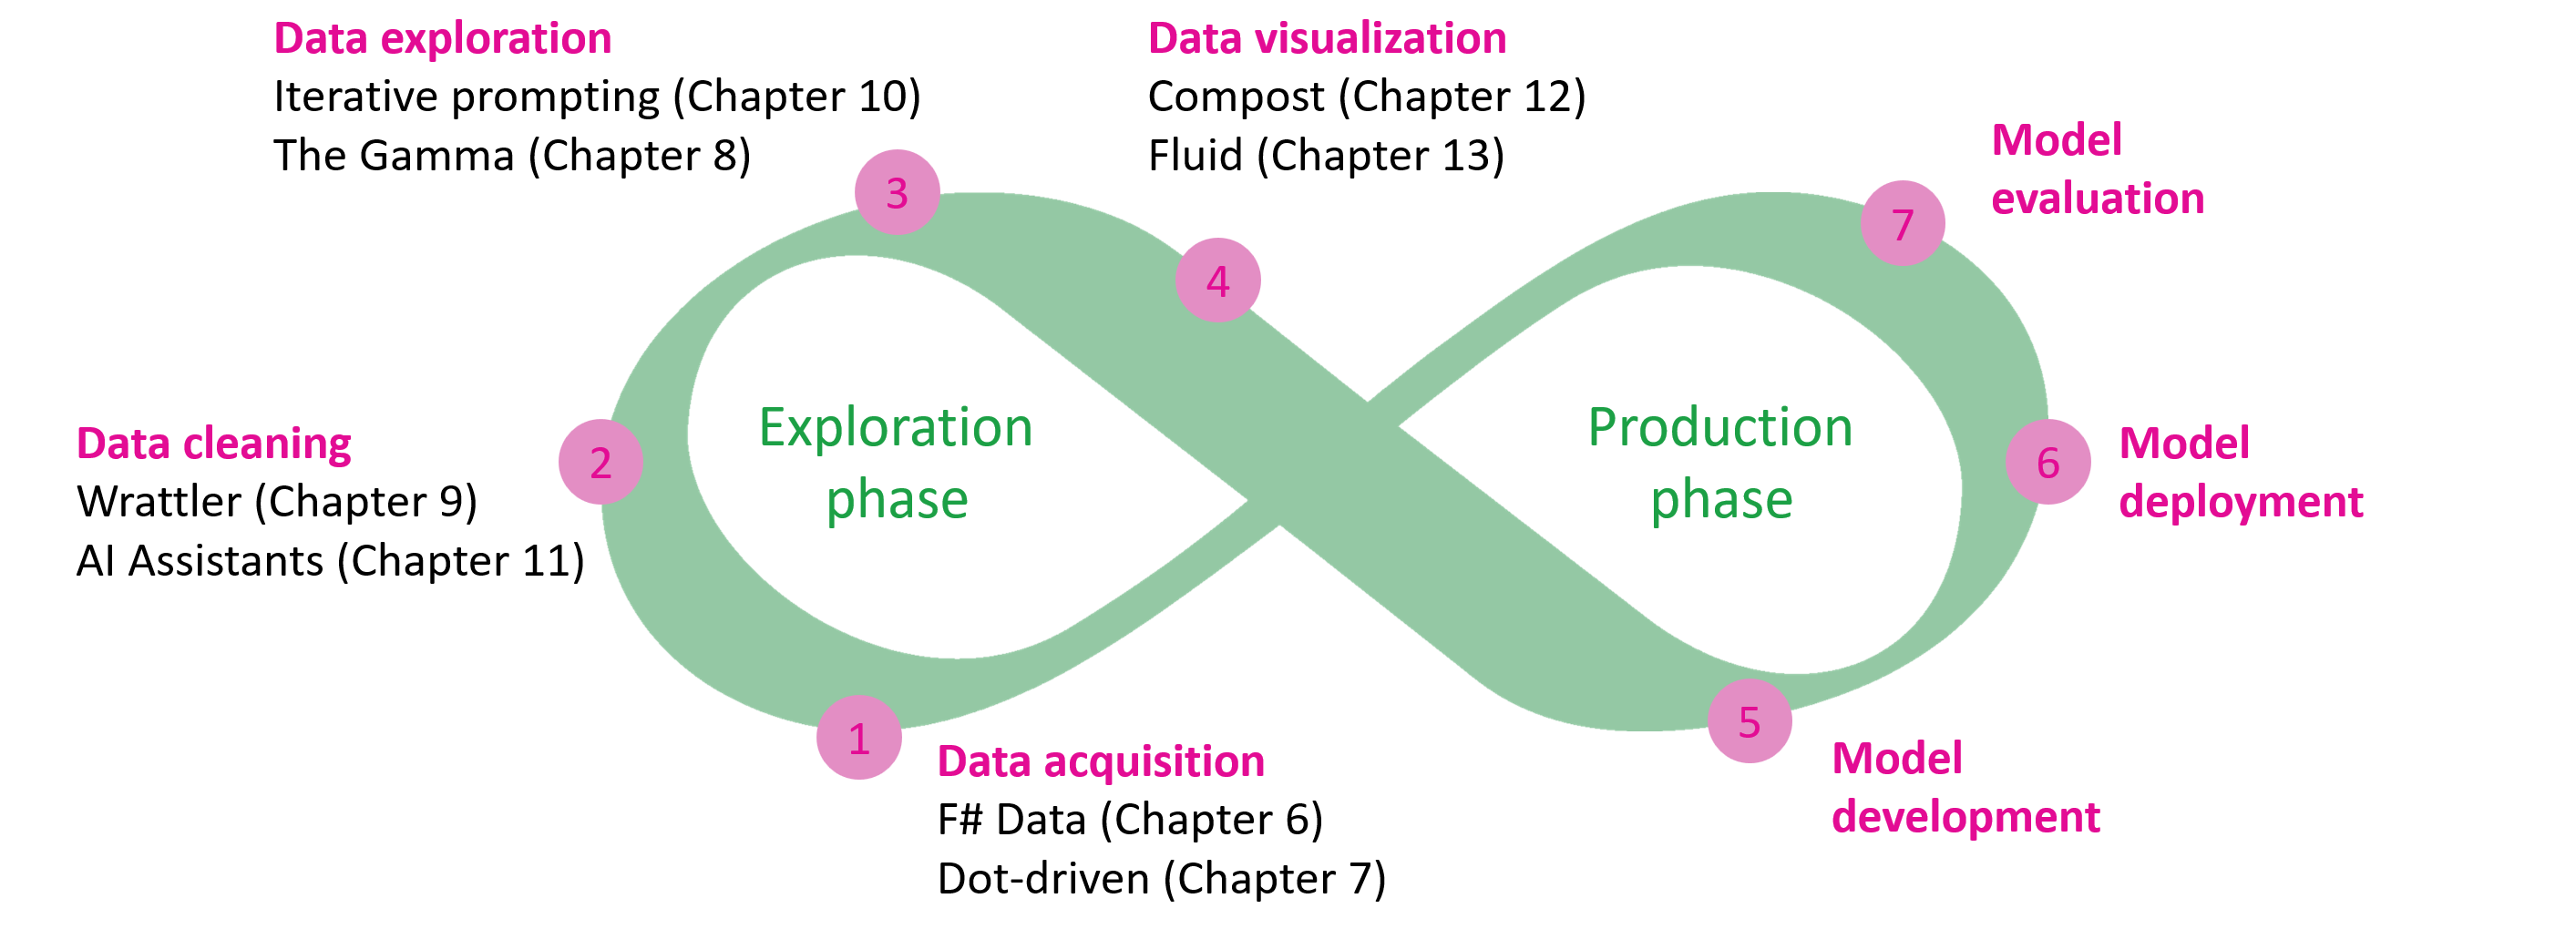
\includegraphics[scale=0.2]{img/lifecycle.png}
  \vspace{-1em}
  \caption{Illustration showing the data science lifecycle, as understood by \cite{ibm-2020-lifecycle},
  alongside with the contributions of this thesis to the individual steps of the data exploration phase.}
  \label{fig:lifecycle}
\end{figure}

The data science lifecycle starts with data acquisition (1), which involves loading
data from a range of sources. This is followed by data cleaning (2), where multiple data sources
are joined, incompete data is filled or removed and data structure is recovered.
In data exploration (3), the analyst transforms the data to discover
interesting patterns and, finally, in data visualization (4) they produce charts to present
their insights. In the production phase, the insights are then used to develop a model
that becomes a part of a production system. The process can be repeated based on the results
of the model evaluation.

The work that constitutes this thesis contributes to each of the four steps of the data
exploration phase. In Part~\ref{part:providers}, I present two papers on type providers,
which simplify data acquisition, while Part~\ref{part:visualization} consists of two
novel data visualization systems. The four publications presented in Part~\ref{part:infra}
and Part~\ref{part:iterative} all focus on working with data, including data cleaning and
exploration. They are not grouped in parts based on the lifecycle step, but based on their research
methodology. The publications in Part~\ref{part:infra} use programming systems methods to
design new infrastructure, while Part~\ref{part:iterative} introduces a novel interaction
principle and applies it to two problems, one from the domain of data exporation and one from the
domain of data cleaning. The rest of this section summarizes the contributions of the work
presented in this thesis in more detail.

\paragraph{Type providers.}
The \emph{type provider} mechanism \citep{syme-2012-providers,syme-2013-inforich} makes it possible
to integrate external data into a statically-typed programming langauge. The work presented in
Part~\ref{part:providers} presents two new type providers.

Chapter~\ref{ch:fsdata} presents a library of type providers that makes it possible to safely access
structured data in formats such as CSV, XML and JSON in the F\# programming language. The two key
research contributions of the work are, first, a novel inference mechanism that infers a type based
on a collection of sample data and, second, a formulation of a \emph{relative safety property} that
formally captures the safety guarantees offered by the system.

Chapter~\ref{ch:dotdriven} takes the idea of type providers further. It uses the mechanism not just
for data access, but for construction of SQL-like queries over tabular data. The research
contribution is a novel type provider, implemented in The Gamma system, which generates a type that
can be used to group, filter and sort tabular data. Using a novel formal model, the presented paper
shows that all queries constructed using the type provider are valid.

\paragraph{Data infrastructure.}
Programmatic data exploration is typically done in notebook systems such as Jupyter
\citep{kluyver-2016-jupyter} that make it possible to combine documentation, formulas, code and
output such as visualizations. Notebook systems are a convenient tool, but they suffer from
a number of limitations and issues. The two novel systems presented in Part~\ref{part:infra} adress
several of those.

Chapter~\ref{ch:foundations} presents a programming environment for The Gamma that makes data
exploration easier by providing instant feedback. The research contributions of the work are
twofold. First, builds a practical efficient algorithm for displaying live previews. Second, it
develops a formal model of code written to explore data called \emph{data exploration calculus}
and uses it to show the correctness of the live preview algorithnm.

Chapter~\ref{ch:wrattler} tackles more directly the problems of notebook systems. It presents
Wrattler, which is a novel notebook system that makes it possible to combine multiple
programming languages and tools in a single notebook, resolves the reproducibility issues of
standard systems and stores computation state in a transparent way, allowing for precise
data provenance tracking.

\paragraph{Iterative prompting}
Treating data analyses as programs makes them transparent and reproducible, but writing code has
an unavoidable basic complexity. Part~\ref{part:iterative} presents a novel interaction principle for
program construction called \emph{iterative prompting}. The mechanism is rooted in the work on type
providers and makes it possible to construct programs by repeatedly choosing from one of several
options.

Chapter~\ref{ch:thegamma} introduces the iterative prompting mechanism from the human-computer
interaction perspective. It shows that the mechanism can be used to construct programs that
explore data in multiple input formats including tables, graphs and data cubes. The usability of
the mechanism is evaluated through a user study, showing that non-programmers can use it to
complete a range of data exporation tasks.

Chapter~\ref{ch:aia} uses the iterative prompting mechanism as the basis of a range of
semi-automatic data cleaning tools. It augments existing AI tools for parsing data, merging data,
inferring data types and semantic information with a mechanism that lets the user guide the AI
tool. Using iterative prompting, the user can correct mistakes and configure parameters of the tool.
The augmented tools are evalauted empirically, showing that the correct result can typically be
obtained with 1 or 2 manual interventions.

\paragraph{Data visualization.}
Data visualization is the last step in the exploratory phase of the data science lifecycle
discussed above. Although standard charts are typically easy to build, creating richer
interactive visualizations is a challenging programming task. Part~\ref{part:visualization}
presents two systems that make it easier to build interactive data visualizations that encourage
critical thinking about data.

Chapter~\ref{ch:compost} presents a functional domain-specific language for creating charts that
makes it possible to compose rich interactive charts from basic building blocks (such as lines
and shapes) using small number of combinators (such overlaying and nesting of scales).
The simplicity of the approach is illustrated through a range of examples and confirmed by the
publication of the work as a so-called functional pearl \citep{gibbons-2010-pearl}.

Chapter~\ref{ch:galois} introduces a language-based program analysis technique that makes it
possible to automatically build linked data visualizations that show the relationships between parts
of charts produced from the same input data. The key research contribution is a novel bidirectional
dynamic dependency program analysis, which is formalised and shown to have a desirable formal
structure. The technique is used as the basis for a high-level programming langauge Fluid.

\section{Open-source software contributions}

The work presented in this thesis is not merely theoretical. An important contribution
of this thesis is a practical implementation of the presented programming systems, languages
and libraries. The concepts discussed in the previous section have been implemented in
several open-source software packages that are available under the permissive Apache 2.0 (F\# Data)
and MIT (all other projects) licenses.

\begin{nitemize}
  \item \emph{F\# Data} (\url{https://github.com/fsprojects/FSharp.Data}) has became a widely-used
    F\# library for data access. It implements utilities, parsers and type providers for working
    with structured data in multiple formats (XML, JSON, HTML and CSV). The initial version based
    on the work presented in Chapter~\ref{ch:fsdata} has since been extended by multiple
    contributors from the F\# community.

  \item \emph{The Gamma} (\url{https://github.com/the-gamma}) is a simple data exploration
    environment for non-programmers such as data journalists. It implements the iterative
    prompting mechanism for data access (Chapters~\ref{ch:thegamma} and \ref{ch:dotdriven})
    and live preview mechanism (Chapter~\ref{ch:foundations}). Live demos using the environment
    in a web browser can  be found at \url{https://thegamma.net} and \url{https://turing.thegamma.net}.

  \item \emph{Wrattler} (\url{https://github.com/wrattler}) is an experimental notebook system
    described in Chapter~\ref{ch:wrattler} that tracks dependencies between cells, makes it
    possible to combine multiple langauges in a single notebook and hosts AI assistants for
    data wrangling described in Chapter~\ref{ch:aia}. More information can be found at
    \url{http://www.wrattler.org}.

  \item \emph{Compost.js} (\url{https://github.com/compostjs}) is a composable library for creating
    data visualizations described in Chapter~\ref{ch:compost}. Although the library is implemented
    in the F\# language, it is compiled to JavaScript and provides a convenient interface for
    Java\-Script users. A range of demos illustrating the use of the library can be found online at
    \url{https://compostjs.github.io}.

  \item \emph{Fluid} (\url{https://github.com/explorable-viz/fluid}) is a programming langauge
    for building linked data visualizations described in Chapter~\ref{ch:galois}. The project has
    since been developed into a general-purpose langauge for transparent, self-explanatory research
    outputs by the Institute of Computing for Climate Science, University of Cambridge.
    A live example can be found at \url{https://f.luid.org}.
\end{nitemize}

% ==================================================================================================
% CHAPTER 2: TYPE PROVIDERS
% ==================================================================================================

\chapter{Type providers}
\label{ch:tp}

The first step of the data science lifecycle outlined in the previous chapter was data acquisition.
This typically involves reading data in semi-structured formats such as CSV, XML and JSON or
retrieving data from a a database. The aim of the work on type providers, outlined in this chapter,
is to make programmatic data acquisition reliable and simpler.

The lack of reliability arises primarily from the fact that most data access code is written in
dynamically-typed scripting languages. This is largely because using such langauges is easier.
A dynamically-typed language does not need to consider the structure of the input data to
check that the program accesses it correctly. If we retrieve a JSON object that represents a record
with fields \texttt{title} and \texttt{link} and parse it into an object \texttt{item} in
JavaScript, we can then access the fields using just \texttt{item.title} and \texttt{item.link}.
The fields will exist at runtime, but the language does not need to know at compile-time whether
they will be  available, because member access is not statically checked.

In statically-typed programming languages, the situation is no better. The typical approach, illustrated
in Figure~\ref{fig:rss}, is equally dynamic, but more verbose. Object fields are accessed using
a string-based lookup, which can easily contain fields that do not exist at runtime (indeed, there
is an uncaught typo on line 6!) and, moreover, the lookup has to be done using an additional method
invocation and may require tedious type coversions. The first challenge we face is how to
make accessing data in semi-structured formats, such as JSON, XML and CSV, as simple as in
dynamically-typed languages (a matter of just using a dot), but support checking that will
statically guarantee that the accessed fields will be present at runtime.

However, the simplicity of data access in dynamic scripting langauge also has its limits. It is easy to
access individual fields, but the code gets more complicated if we want to perform a simple
query over the data. Consider, for example, the query in Figure~\ref{fig:pandas}.

\begin{figure}[h!]
\vspace{-0.33em}
\begin{lstlisting}[language=sharp]
var url = "http://dvd.netflix.com/Top100RSS";
var rss = XDocument.Load(topRssFeed);
var channel = rss.Element("rss").Element("channel");

foreach(var item in channel.Elements("item")) {
  Console.WriteLine(item.Element("titel").Value);
}
\end{lstlisting}
\vspace{-0.33em}
\caption{Printing titles of items from an RSS feed in C\#. The snippet uses dynamic lookup to
find appropriate elements in the XML and extracts and prints the title of each item.}
\label{fig:rss}
\end{figure}

\begin{figure}[t]
\begin{lstlisting}[language=ppython]
olympics = pd.read_csv("olympics.csv")
olympics[olympics["Games"] == "Rio (2016)"]
  .groupby("Athlete")
  .agg({"Gold": sum})
  .sort_values(by="Gold", ascending=False)
  .head(8)
\end{lstlisting}
\caption{Data transformation written using pandas in Python. The code loads a CSV file with
Olympic medal history, gets data for Rio 2016 games, groups the data by athlete and sums their
number of gold medals and, finally, takes the top 8 athletes.}
\label{fig:pandas}
\end{figure}

Despite being widely accepted as simple, the Python code snippet involves a remarkable number
of concepts and syntactic elements that the user needs to master:

\begin{nitemize}
\item \emph{Generalised indexers} (\texttt{.[ condition ]}) are used to filter the data. This is
  further complicated by the fact that \texttt{==} is overloaded to work on a data series and the
  indexer accepts a Boolean-valued series as an argument.
\item \emph{Python dictionaries} (\texttt{\{"key": value\}}) are here used not to specify a lookup
  table, but to define a list of aggregation operations to apply on individual columns. It also
  determines the columns of the returned data table.
\item \emph{Well-known names}. The user also has to remember the (somewhat inconsistently named)
  names of operations such as \texttt{groupby} and \texttt{sort\_values} and remember the
  column names from their data source such as \texttt{"Athlete"}.
\end{nitemize}

To make data acquisition simpler, the user should not need this many concepts and they should not
need to remember the names of operations or the names of columns in their data source.
Moreover, their code should be checked to ensure that it accesses the correct supported
operations and applies them on compatible data that exist in the data source. As I will show later,
this can be achieved using type providers, a concept that originated in the F\# programming language
in the early 2010s.

\section{Information-rich programming}
In the 2010s, applications increasingly relied on external data sources and APIs for their
function. The typical solution for accessing such data was either to use a scripting language,
a dynamic access library (both illustrated above) or a code-generation tool that would generate
code for accessing the data source or an API (although only for data sources with small enough
schema). This provided the motivation for the type provider mechanism in F\#
\citep{syme-2012-providers,syme-2013-inforich}, which made it possible to make the type checker
in a statically-typed programming language aware of the structure of external data sources.

Technically, a type provider in F\# is an extension that is executed by the compiler at
compile-time. A type provider can run arbitrary code, such as access read a database schema or
access another external data source. It then generates a representation of a type that is
passed to the compiler and used to check the user program. For example, the World Bank
type provider (Figure~\ref{fig:wb}) retrieves the list of known countries and indicators from
the World Bank database (by querying the REST API provided by the World Bank) and generates
a collection of types. The \texttt{WorldBank} type has a \texttt{GetDataContext} method, which
returns an instance of a type with the \texttt{Countries} member and the type returned by this
member has one member corresponding to each country in the World Bank database.
The World Bank type provider, created by the auhtor of this thesis and presented in a report
\citep{syme-2012-providers} not included here, shows two important properties of type providers:

\begin{figure}[t]
\begin{lstlisting}[language=sharp]
type WorldBank = WorldBankDataProvider<"World Development Indicators">
let data = WorldBank.GetDataContext()

data.Countries.``United Kingdom``.Indicators
  .``Central government debt, total (% of GDP)``
\end{lstlisting}
\vspace{-0.5em}
\caption{The World Bank type provider \citep{syme-2012-providers} provides access to indicators
collected by the World Bank. The countries and indicators are mapped to properties (members)
of an F\# class that represents the data.}
\vspace{-0.5em}
\label{fig:wb}
\end{figure}

\begin{nitemize}
\item \emph{Static type provider parameters.} A type provider in F\# can take literal values
  (such as \texttt{"World Development Inicators"}) as parameters. They can be used when the provider
  is executed (at compile-time) to guide how types are generated. Here, the parameter specifies
  a particular database to use as the source. These can be names of files with schema, connection
  strings or live URLs.

\item \emph{Lazy type generation.} The types generated by a type provider are generated lazily, i.e.,
  the members of a type (and the return types of those members) are only generated when the type
  checker encounters the type in code. This makes it possible to import very large (potentially
  infinite) external schema into the type system.
\end{nitemize}

There are other interesting aspects of type providers, but the above two features are crucial
for the work included in this thesis. In the following two sections, I review the key contributions
to type providers presented in Part~\ref{part:providers} make data acquisition reliable
and simpler.
%
The work on type providers included in this thesis develops two kinds of type providers.
The type providers for CSV, JSON and XML packaged in the F\# Data library make it possible
to access data in a statically-checked way using ordinary member access. The work also makes
two theoretical contributions, an algorithm for schema inference from sample data and a
programming langugae theory of type providers.

The pivot type provider, developed for the experimental programming language The Gamma,
makes it possible to construct queries such as that shown in Figure~\ref{fig:pandas} (and
was mentioned briefly in Section~\ref{sec:intro-ddj}). It adapts the theory developed for the
F\# Data type providers to show that only correct queries can be constructed when using it.
%
The full account of the work can be found in Chapter~\ref{ch:fsdata} and
Chapter~\ref{ch:dotdriven}, respectively. The following provides an accessible high-level overview
of the contributions.

\section{Type providers for semi-structured data}
The F\# Data library implements type providers for accessing data in XML, JSON and CSV formats.
It is based on the premise that most real-world data sources using those formats do not have an
explicit schema. The type providers thus infer the schema from a sample (or a collection of
samples). The inferred schema is then mapped to F\# types through which the user of the type
provider can access the data.

\begin{figure}[t]
\begin{lstlisting}[language=sharp]
// worldbank.json - a sample response used for schema inference
[ { "page": 1, "pages": 1, "per_page": "1000", "total": 53 },
  [ { "indicator": { "id": "GC.DOD.TOTL.GD.ZS" },
      "country": { "id": "CZ" },
      "date": "2011", "value": null },
    { "indicator": { "id": "GC.DOD.TOTL.GD.ZS" },
      "country": { "id": "CZ" },
      "date": "2010", "value": 35.1422970266502 } ] ]
\end{lstlisting}
\begin{lstlisting}[language=sharp]
// demo.fsx - a data acquisition script using a type provider
type WB = JsonProvider<"worldbank.json">
let wb = WB.Load("http://api.worldbank.org/.../GC.DOD.TOTL.GD.ZS?json")

printf "Total: %d" wb.Record.Total
for item in wb.Array do
  match item.Value with
  | Some v -> printf "%d %f" item.Date v
  | _ -> ()
\end{lstlisting}
\caption{Using the .JSON type provider for accessing data from a REST API. The inference uses
a local sample file, while at runtime, data is obtained by calling the live service.}
\label{fig:json}
\end{figure}

The example shown in Figure~\ref{fig:json} illustrates one typical use. Here, the user is
accessing information from a service that returns data as JSON (incidentally, the service is also
the World Bank, but here we treat it as an ordinary REST service). The user stored a local copy
of a sample response from the service (\texttt{worldbank.json}) and uses it as a static parameter
for the JSON type provider (line 2). They then load data from the live service (line 3)
and print the total number of items (line 5) as well as each year for which there is a value
(line 8). Three aspects of the type provider deserve particular attention:

\begin{nitemize}
\item \emph{Real-world schema inference is hard.} Here, the response is an array always containing
  two items, a record with meta-data and an array with individual data points. The data records
  have consistent structure, although some values may be \kvd{null}.
\item \emph{Inference needs to be stable.} The type providers allow adding further samples. If the
  user adds further examples, the structure of the provided types should change in a predictable
  (and limited) way so that the user code can be easily updated.
\item \emph{Safety guaranteed by static checks is relative.} Static type checking guarantees that
  only data available in the sample input can be accessed in user code, but if the data loaded at
  runtime have different structure, this will not prevent errors. We thus need to specify what
  exactly can the system guarantee about programs.
\end{nitemize}

The F\# Data type providers, presented in full in Chapter~\ref{ch:fsdata} offer an answer to
all of these three challenges. They can infer shape of real-world data, infer types with a stable
structure and capture the runtime guarantees formally through the relative safety property. The
publication also presented novel programming language theory that made it possible to analyze type
providers formally, which I briefly review in the next three sections.

\subsection{Shape inference and provider structure}
When the type provider for semi-structured data is used, it is given a sample of data that
can be analysed at compile time (such as the \texttt{"worldbank.json"} file name above). It
uses this to infer the shape of the data. A shape is a structure similar to a type and is
composed from primitive shapes, record shapes, collections and a few other special shapes:
%
\begin{equation*}
\begin{array}{rcl}
 \hat{\sigma} &=& \nu \; \{ \nu_1 \!:\! \sigma_1, \,\ldots\,, \nu_n \!:\! \sigma_n \}\\
                &|& \ident{float} \lsep \ident{int} \lsep \ident{bool} \lsep \ident{string}\\
       \sigma &=& \kvd{nullable}\langl \hat{\sigma} \rangl \lsep [\sigma] \lsep \kvd{any} \lsep \kvd{null}  \lsep ~\bot~
\end{array}
\end{equation*}
%
The inference distinguishes between non-nullable shapes ($\hat{\sigma}$) and nullable shapes
($\sigma$), which can be inferred even when the collection of inputs contains the \kvd{null}
value. The former consist of primitive shapes (inferred from a corresponding value) and
a record shape. The record shape has an (optional) name $\nu$ and consists of a multiple fields
that have their own respective shapes. A record is the shape inferred for JSON objects, but also
XML elements containing attributes and child elements. A non-nullable shape can be made nullable
by explicitly wrapping it as $\kvd{nullable}\langl \hat{\sigma} \rangl$. Other nullable shapes
include collections (a \kvd{null} value is treated as an empty collection) and shapes that represent
any data, only null values and the bottom shape $\bot$, representing no information about the shape.
The anove definition does not include handling of choice shapes (corresponding to sum types), which
is introduced later.

A key techincal operation of the shape inference is expressed using the \emph{common preferred shape}
function written as $\sigma_1 \triangledown \sigma_2 = \sigma$. Given two shapes, the function
returns a shape the most specific shape that can be used to represent values of both of the two
given shapes. The details are discussed later, but it is worth illustrating how the function works
using two examples.

\begin{nitemize}
\item $\ident{int} \,\triangledown\, \ident{float} = \ident{float}\quad$ In this case, the common
  preferred shape is \ident{float}. This may lead to a loss of precision, but it makes accessing
  the data easier than if we inferred a shape representing a choice shape. This is one example
  where the system favors practical usability over formal correctness.
\item $\{ \textit{x} \!:\! \ident{int} \} \,\triangledown\,
  \{ \textit{x} \!:\! \ident{int}, \textit{y} \!:\! \ident{int} \} =
  \{ \textit{x} \!:\! \ident{int}, \textit{y} \!:\! \kvd{nullable}\langl\ident{int}\rangl \}\quad$
  In this case, the common preferred shape is a record where the field that was missing in one
  of the shapes is marked as \kvd{nullable}. In general, the system aims to infer records whenever
  possible, which is the key for the stability of inferred types discussed below.
\end{nitemize}

When the type provider is used, it receives a sample data value and uses it to infer the expected
shape of data. A data value is modelled formally as a value that can be either a primitive value
(integer $i$, floating-point value $f$, string $s$, a Boolean or \kvd{null}), a collection of values
or a record with fields that have other values:
%
\begin{equation*}
\begin{array}{lcl}
  \\[-0.5em]
 d &=& i \lsep f \lsep s \lsep \kvd{true} \lsep \kvd{false} \lsep \kvd{null} \\[0.1em]
   &|& [d_1; \ldots; d_n] \lsep \nu~\{ \nu_1 \mapsto d_1, \ldots, \nu_n \mapsto d_n \}
\end{array}
\end{equation*}
%
The shape inference is then defined as a function $\semalt(d_1, \ldots, d_n)=\sigma$ that takes a
collection of data values and infers a single shape $\sigma$ that represents the shape of all the
specified values. (Note that this can always be defined. In case where values are of incompatible
shape, the system infers the shape $\kvd{any}$.)

\begin{equation*}
\begin{array}{rclcrclcrcl}
 \semalt{i} &=& \ident{int} && \semalt{\kvd{null}}  &=& \kvd{null} && \semalt{\kvd{true}} &=& \ident{bool}\\[0.3em]
 \semalt{f} &=& \ident{float} && \semalt{s} &=& \ident{string} && \semalt{\kvd{false}}  &=& \ident{bool}\\
\end{array}
\end{equation*}
\noindent
\vspace{-0.6em}
\begin{equation*}
\begin{array}{l}
 \semalt{[d_1; \ldots; d_n]} = [\semalt{d_1, \ldots, d_n}] \\[0.5em]
 \semalt{\nu~\{ \nu_1 \mapsto d_1, \ldots, \nu_n \mapsto d_n \}} = \nu~\{ \nu_1:\semalt{d_1}, \ldots, \nu_n :\semalt{d_n} \} \\[0.5em]
 \semalt{d_1, \ldots, d_n} = \sigma_n ~\textnormal{where}~ \sigma_0 = \bot,~ \forall i\in \{ 1.. n \}.~ \sigma_{i-1} \triangledown \semalt{d_i} \vdash \sigma_i \\[0.6em]
\end{array}
\end{equation*}
%
The shape inference is primarily defined on individual data values. For those, the system infers
the shape corresponding to the value. For lists, we infer the shape based on all the values in
the list. Finally, the last rule handles multiple sample data values by inferring their individual
shapes and combining them using the  $\triangledown$ function.

The last aspect of the formal programming language model of type providers is the logic that,
given an inferred shape, produces the corresponding F\# type. To explain the important
properties of type providers, we do not need to elaborate what an F\# type is here, but the most
important case is a class with members (properties or methods). A type provider takes the inferred
shape and produces an F\# type $\tau$ for the shape, a collection of classes $L$ that may appear
in $\tau$ (typically as types of members in case $\tau$ is a class). The type provider also needs
to generate code that turns a raw data value $d$ passed as input at runtime into a value of the
provided type $\tau$, which is represented as an expression $e$:
%
\begin{equation*}
\sem{\sigma} = (\tau, e, L) \qquad (\textnormal{where}~L,\emptyset \vdash e:\ident{Data}\rightarrow\tau)
\end{equation*}
%
The mapping $\sem{\sigma}$ takes an inferred shape $\sigma$ and returns a tripple consisting of an
F\# type $\tau$, a function turning a data value into a value of type $\tau$ and a collection of
classes $L$.

This brief overview of the formal model of type providers for semi-structured data makes it possible
to formulate the two key results about the F\# Data type providers. The first describes the relative
type safety of programs written using a type provider and is a novel variation on the classic
type safety property of programming langauge research. The second describes the
stability of provided types and concerns usability of the system.

\subsection{Relative safety of checked programs}

The aim of type systems, in general, is to ensure that programs which passed type checking do not
contain a certain class of errors. This has been characterised by \citet{milner-1978-gowrong}
using a famous slogan ``Well typed programs do not go wrong'' (with \textit{wrong} being a formal
entity in Milner's system). A code written using a type provider can go wrong if the
input obtained at runtime is of a structure that does not match the structure of the input used
as a sample for shape inference at compile time.

However, thanks to the formal model defined above, the property can be specified precisely and,
most importantly, we can specify for which inputs the programs written using a type provider will
never fail because of invalid data access. The definition relies on a preferred shape relation
$\sqsubseteq$, which captures the fact that one shape is more specific than another (if
$\sigma_1 \sqsubseteq \sigma_2$ then $\sigma_1 \triangledown \sigma_2 = \sigma_2$).
%
The theorem is also defined in terms of the $\reduce$ operation, which captures the operational
semantics of the programs of the language used in the formal model. The relation $e_1 \reduce e_2$
specifies that an expression $e_1$ reduces to $e_2$ in a single step (and $\reduce^{*}$ is the
transitive closure of $\reduce$).

\begin{theorem}[Relative safety]
\label{thm:safety}
Assume $d_1, \ldots, d_n$ are samples, $\sigma=\semalt{d_1, \ldots, d_n}$ is an inferred
shape and $\tau,e,L = \sem{\sigma}$ are a type, expression and class definitions generated by a
type provider.

For all inputs $d'$ such that $\semalt{d'} \sqsubseteq \sigma$ and all expressions $e'$
(representing the user code) such that $e'$ does not contain any of the dynamic data operations $op$
and any \ident{Data} values as sub-expressions and $L; y\!:\!\tau \vdash e'\!:\!\tau'$, it is
the case that $L, e[y\leftarrow e'~d'] \reduce^{*} v$ for some value $v$ and
also $\emptyset; \vdash v : \tau'$.
\end{theorem}
\vspace{-0.2em}

In other words, the relative safety property specifies that, for any program that the user may
write using a type provider (without using low-level functions that are only usable accessible
inside a type provider), if the program is executed with any input whose shape is more specific
than the shape inferred from statically known samples, the program will not encounter a data-related
runtime error. It is, of course, still possible for runtime errors to happen, but not with a
well-chosen sample and, as the wide-ranging adoption of the F\# Data library suggests,\footnote{The
package is one of the most downloaded F\# libraries at the \url{https://www.nuget.org} package
repository and the open-source project at \url{https://github.com/fsprojects/FSharp.Data} has
over 100 contributors.} this is often a sufficient guarantee in practice.

\subsection{Stability of provided types}
When the user of an F\# Data type provider gets a runtime error, this is because the
data source they use produced an input of a structure not encountered before. A typical example
is an input that includes \kvd{null} in a field that previously always had a value.
Such errors are inevitable (without an explicit schema). The programmer can handle this by
adding the new input as a new sample to the collection of samples used for the shape inference.

If they do so, the type provider will provide a new different type. In this case, an important
property of the system is that the newly provided type will have the same general structure as
the type provided before. This means that the data processing code, written using the provided
type, will be easy to adapt. The programmer will need to add handling of a missing value, but
they will not have to restructure their code. (A system based on statistical analysis of similarity
would not have this property as a small change in the input may affect a decision whether two
shape are sufficiently similar to be unified into a single type.) Using the formal model, we
can capture this property (and later prove that it holds for the F\# Data type providers).

\begin{theorem}[Stability of inference]
Assume we have a set of samples $d_1, \ldots, d_n$, a provided type based on the samples
$\tau_1, e_1, L_1 = \sem{\semalt{d_1, \ldots, d_n}}$ and some user code $e$ written using
the provided type, such that $L_1; x:\tau_1\vdash e : \tau$.
%
Next, we add a new sample $d_{n+1}$ and consider a new provided type
$\tau_2, e_2, L_2 = \sem{\semalt{d_1, \ldots, d_n, d_{n+1}}}$.

Now there exists $e'$ such that $L_2; x:\tau_2\vdash e' : \tau$ and if
for some $d$ it is the case that $e[x\leftarrow e_1~d] \reduce v$ then
also $e'[x\leftarrow e_2~d] \reduce v$.
%
Such $e'$ is obtained by transforming sub-expressions of $e$ using one of the following
translation rules:
%
\vspace{-0.1em}
\begin{enumerate}[(i)]
\itemsep -0.1em
\item $C[e]$ to $C[\kvd{match}~e~\kvd{with}~\ident{Some}(v) \rightarrow v~|~\ident{None} \rightarrow \ident{exn}]$
\item $C[e]$ to $C[e.\ident{M}]$ where $\ident{M} = \tytagof(\sigma)$ for some $\sigma$
\item $C[e]$ to $C[\ident{int}(e)]$
\end{enumerate}
\end{theorem}
%
The translation rules use a context $C[e]$ to specify that a transformation needs to be done
somewhere in the program. Importantly, all the rules are \emph{local} meaning that a change
is done in a particular place in the program. The change can be (i) handling of missing value,
(ii) accessing a newly introduced member when the change introduces a new choice type
and (iii) adding a conversion of a primitive value.

\section{Type providers for query construction}
\label{sec:tp-query}

The type providers presented in the previous section are designed to allow easy programmatic
access to data in semi-structured formats. The focus is on providing typed direct access to the
data. The pivot type provider, presented in Chapter~\ref{ch:dotdriven}, builds on the same
concepts, but focuses on letting users construct queries over tabular data. The user should not
just be able to fetch the data in a typed form, but also use the provided types to filter,
aggregate and reshape the data.

\begin{figure}[t]
\vspace{-0.5em}
\begin{lstlisting}[language=sharp]
olympics
  .'filter data'.'Games is'.'Rio (2016)'.then
  .'group data'.'by Athlete'.'sum Gold'.then
  .'sort data'.'by Gold descending'.then
  .'paging'.take(8)
\end{lstlisting}
\vspace{-0.25em}
\caption{Data transformation constructed using the pivot type provider. This implements the
same logic as pandas code in Figure~\ref{fig:rio}, computing the top 8 athletes from the Rio 2016
Olympic games based on their number of gold medals.}
\label{fig:rio}
\vspace{-0.25em}
\end{figure}

The use of the pivot type provider is illustrated in Figure~\ref{fig:rio}, which implements
the data querying logic written using the pandas Python library in Figure~\ref{fig:pandas}.
The type provider is implemented in the context of The Gamma programming language, which is a
simple statically typed programming language with class-based object model and type providers
that runs in the web browser.

As the code sample shows, the querying is implemented as a single chain of member accesses.
Except for \texttt{take}, which is a method with a numerical parameter, all the members are
properties that return another object of another class type with furhter members that can be
used to continue constructing the query (the symbol \texttt{'} is used to wrap names containing
a space). The system has a number of properties:

\begin{nitemize}
\item \emph{Discoverability of members.} All querying logic is expressed through member accesses.
  The members are statically known (generated by a type provider). When using the type provider in
  an editor, the user gets a choice of available members (auto-completion) when they type ``.''
  and they can thus construct query simply by repeatedly choosing one of the offered members.

\item \emph{Lazy class generation.} The classes used in the code are generated lazily. This is
  necessary, because each operation transforms the set of available fields based on which the
  subsequent types are generated. For example, calling \texttt{'drop Games'} would remove the field
  \texttt{Games} from the schema.

\item \emph{Safety of generated types.} Any query constructed using the type provider is correct meaning that it
  will not attempt to access a field that does not exist in the data. This is a variant of the
  usual type safety property that is formalized below.
\end{nitemize}

The formalization of the type provider follows the same style as that for F\# Data, but it explicitly
encodes the laziness of the type provider as illustrated in the next section.

\subsection{Formalizing lazy type provider for data querying}
The pivot type provider works on tabular data. In order to generate a type, it needs to have the
schema of the input table (names of fields and their types). In the above example, the type
provider is imported through a configuration rather than code and \texttt{olympics} refers to a
value of the provided type, but the type is generated using a known schema of the input data.
In the formal model, the schema is written as (with $f$ ranging over the field names and
$\tau$ ranging over a small set of primitive types):
%
\begin{equation*}
F=\{ f_1 \mapsto \tau_1, \ldots, f_n \mapsto \tau_n \}
\end{equation*}
%
When the type provider is invoked, it takes the schema and generates a class for querying data
of the given schema. The types of the members of the class are further classes that allow further
querying. As the provided class structure is potentially infinite, it needs to be generated
lazily. The structure of provided class definition, written as $L$ is thus a function mapping
a class name $C$ to a pair consisting of the class definition and a function that provides
definitions of delayed classes (types used by the members of the class $C$):
%
\begin{equation*}
L(C) = \kvd{type}~C(x:\tau) = \overline{m}, L'
\end{equation*}
%
Here, $\kvd{type}~C(x:\tau) = \overline{m}$ is a definition of a class $C$ that consists of a
sequence of members $\overline{m}$ and has a constructor taking a variable $x$ of type $\tau$ as
an argument. The structure and evaluation of the resulting object calculus is discussed
in Chapter~\ref{ch:dotdriven} and is loosely modelled after standard object calculi
\citep{igarashi-2001-fj,abadi-2012-objects}, with the exception that it includes
operations for transforming data as primitives.

The classes provided by the pivot type provider can be used to construct a query, which is a
value of type \ident{Query}. Expressions of this type are those of the relational algebra
(projection, sorting, selection, as well as additional grouping). The type provider constructs
classes that take the query constructed so far as the constructor argument. The provided members
further refine and build the query. A type provider is formally defined as a function
$\ident{pivot}(F)$, which is similar to the function $\sem{\sigma}$ defined for the F\# Data
type providers:
%
\begin{equation*}
\begin{array}{l}
\ident{pivot}(F) = C, \{ C \mapsto (\kvd{type}~C(x:\ident{Query}) = \ldots,L) \}\\
  \qquad \textnormal{where}~F=\{ f_1 \mapsto \tau_1, \ldots, f_n \mapsto \tau_n \}
\end{array}
\end{equation*}
%
The full definition given in Chapter~\ref{ch:dotdriven} uses a number of auxiliary functions to
define the type provider, each of which defines members for specifying a particular query operation.
To illustrate the approach, the following excerpt shows the $\ident{drop}(F)$ function that is used
to construct operations that let the user drop any of the columns currently in the schema $F$.
The generated class has a member \qident{drop $f$} for each of the fields and a memebr
\ident{then}, which can be used to complete the selection and return to the choice of other query
operations. Each of the \ident{drop} operations returns a class generated for the newly restricted
domain and passes it a query that applies the selection $\Pi$ operation of the relational algebra
on the input data:
%
\begin{equation*}
\begin{array}{ll}
\ident{drop}(F) = C, \{ C \mapsto (l, L' \cup \bigcup L_f) \}\qquad\\[0.5em]
l = \kvd{type}~C(x:\ident{Query}) = &\hspace{-1em}\forall f \in \ident{dom}(F)~\textnormal{where}~C_f, L_f = \ident{drop}(F')\\
~~\qquad \kvd{member}~\qident{drop $f$} : C_f = C_f(\Pi_{\ident{dom}(F')}(x)) & \quad\textnormal{and}~ F' = \{ f'\mapsto\tau'\in F, f' \neq f\}\\
~~\qquad \kvd{member}~\ident{then} : C' = C'(x)\qquad                 &\textnormal{where}~C', L' = \ident{pivot}(F)\\
\end{array}
\end{equation*}

The formalization of the pivot type provider follows a similar style as that of the F\# Data,
although it differs in that it explicitly represents the laziness of the type generation and
also in that the provided types construct more complex code, expressed using a a variant of
relational algebra, that is executed at runtime. The formalization serves to explain the functioning
of the type provider, but also allows us to prove its safety.

\subsection{Safety of data acquisition programs}

The pivot type provider guarantees that the data transformations, which can be constructed using
the types it generates and are expressed using the primitives of the relational algebra, will
always be correct. They will never result in an undefined runtime behaviour that one may otherwise
encounter when accidentally accessing a non-existent field. This is important result, because the
sequence of operations transforms the fields in an interesting way. Operations like \texttt{drop}
remove fields from the schema, while \texttt{group by} not only changes the set of fields, but also
their types (e.g., when we count distinct values of a string-typed field $f$ in aggregation,
the resulting dataset will contain a numerical field $f$).

To capture the property formally, we again state that any program written by the programmer using
the type provider (without directly accessing the low-level operations of the relational algebra)
will always reduce to a value. The evaluation is defined on datasets $D$ which
map fields to vectors of values, written as $D =
\{ f_1\mapsto\vect{v_{1,1},\ldots,v_{1,m}}, \ldots, f_n\mapsto\vect{v_{n,1},\ldots,v_{n,m}} \}$.
A specific kind of data value is a data series $\ident{series}\langl\tau_k,\tau_v\rangl(D)$ that
contains a vector of keys $k$ and a vector of values $v$. The evaluation is defined as a reduction
operation $e \leadsto_{L}^{*} e'$ which also has access to class definitions $L$.
Similarly, the typing judgment $L_1;\Gamma \vdash e : \tau; L_2$ includes additional handling of
lazily generated classes. It states that the expression $e$ has a type $\tau$ in a variable context
$\Gamma$. The typing is provided with (potentially unevaluated) class definitions $L_1$. It
accesses (and evaluates) some of those definitions and those that are used throughout the typing
derivation are represented by~$L_2$.

\begin{theorem}[Safety of pivot type provider]
\label{thm:pivot-safe}
Given a schema $F=\{f_1\mapsto\tau_1, \ldots, f_n\mapsto\tau_n \}$, let $C,L=\ident{pivot}(F)$ then for any
expression $e$ that does not contain relational algebra operations or $\ident{Query}$-typed values as sub-expression,
if $L;x\!:\!C \vdash e : \ident{series}\langl\tau_1,\tau_2\rangl; L'$ then for all $D =
\{ f_1\mapsto\vect{v_{1,1},\ldots,v_{1,m}}, \ldots, f_n\mapsto\vect{v_{n,1},\ldots,v_{n,m}} \}$
such that $\vdash v_{i, j} : \tau_i$ it holds that $e[x\leftarrow C(D)]\leadsto_{L'}^{*}
  \ident{series}\langl\tau_k,\tau_v\rangl(\{ f_k\mapsto{k_1,\ldots,k_r}, f_v\mapsto{v_1,\ldots,v_r} \})$
  such that for all $j$ $\vdash k_j : \tau_k$ and $\vdash v_j : \tau_v$.
\end{theorem}

In other words, if a programmer uses the provided types to write a program $e$ that evaluates to
a data series and we provide the program with input data $D$ that matches the schema used to invoke
the type provider, the program will always evaluate to a data series containing values of the
correct type. Although the property is not labelled as \emph{relative type safety} as in the
case of the F\# Data type providers, it follows the same spirit. A well-typed program will not
go wrong, as long as the input has the right structure.

\section{Conclusions}
In this chapter, I offered a brief overivew of the work on type providers that is included in
Part~\ref{part:providers} of this thesis. The focus of this part is on simplifying programmatic
data acquisition, that is on making it easier and safer to write code that reads data from external
data sources. It consists of a type provider for accessing semi-structured data in XML, JSON and
CSV formats (Chapter~\ref{ch:fsdata}) and the pivot type provider that makes it possible to
express queries over tabular data (Chapter~\ref{ch:dotdriven}).

Both of the contributions consist of a practical implementation, as a library for the F\# language and
as a component of the web-based programming environment The Gamma, respectively. They combine this
with a theoretical analysis using the methodology of theoretical programming language research.
This makes it possible to precisely capture subtle aspects of how the type providers work
(including shape inference, laziness and generation of types for query construction), but also
to capture safety guarantees of the generated types. Given that type providers always access
external data, the guarantees are not absolute as in conventional programming language theory.
For this reason, my work introduced a novel notion of \emph{relative type safety}, stating that
programs will ``not go wrong'' as long as the input has correct structure (in a precisely defined
sense).

From a broader perspective, the two type providers can be seen as filling a glaring gap in the
theoretical work of statically-typed programs. A theoretician who defines a type system always uses
a top-level typing rule \,$\vdash\!e\!:\!\tau$\, stating that a program $e$ (closed expression) that
does not use any variables has a type $\tau$. While at the top-level, programs may not use any variables,
this is misleading because most real-world programs access the outside world in some way, but
this is typically done in an unchecked way. Monads and effect systems \citep{lucassen-1988-effects,spj-1993-imperative}
can be used to track that some external access is made, but they do not help the static type
system understand the structure of the outside data.
%
With a slight notational creativity, we can say that the static type checking of a program that
uses type providers starts with a rule $\pi(\oplus) \vdash e\!:\!\tau$ where $\oplus$ (used as the
astronomical symbol for the Earth) refers to the entire outside world and $\pi$ refers
to some projection from all the things that exist in the outside world to program variables
with static types that a programming language understands.

The two kinds of type providers discussed in this chapter also differ in how they approach the
technology gap suggested in Figure~\ref{fig:gap}. The F\# Data type providers aim to make
programming with external data in a statically typed programming langauge a bit easier.
In other words, they extend the area that can be covered by conventional programming,
including more users and reducing the complexity. The pivot type provider and The Gamma
programming environment tries to fill a particular space within the gap. It lets relatively
large number of users (who are not professional programmers) solve problems that are more complex
than simple data wrangling in a spreadsheet system, but much less complex than using a conventional
programming tool such as Python and pandas. Its usability is a topic I will revisit in
Chapter~\ref{ch:iterative} and the paper included as Chapter~\ref{ch:thegamma}.

% ==================================================================================================
% CHAPTER 3: DATA INFRASTRUCTURE
% ==================================================================================================

\chapter{Data infrastructure}
\label{ch:infra}

Data scientists use a wide range of tools when working with data. A large part of what makes
data cleaning and data exploration challenging is that data scientists often need to switch
from one tool to another \citep{rattenbury-2017-wrangling}. They may use an interactive online
tool like Trifacta to do data cleanup, run an ad-hoc command-line tool to
transform it and then import it into a Jupyter notebook to create a visualization. Moreover,
data science is an interactive and iterative process. Data scientist need to be able to quickly
review the results of the operation they performed in order to see whether the results match
their expectations and to detect unexpected problems. The interactivity brings a further challenge,
which is the reproducibility of results. If the data scientist quickly tries multiple different
approaches, reverts some of their earlier experiments, they should always be able to know what
exact steps led to the final result they see on their screen.

In this chapter, I provide overview of two contributions to the infrastructure for doing data
exploration. The work addresses the three requirements that arise from the typical way data
exploration is done as outlined above:

\begin{nitemize}
\item \emph{Polyglot tooling support.} Data scientist need an easy way of integrating multiple
  different tools. For example, they should be able to use a simple data acquisition tools,
  such as the pivot type provider implemented in The Gamma, but then pass the data to Python
  for further processing or to a visual interactive tool.

\item \emph{Live preview support.} In order to let data scientists quickly review the results
  of the operations they perform, the infrastructure should provide immediate live previews
  without unnecessary recomputation.

\item \emph{Reproducibility and correctness.} The results that the data scientist sees on the
  screen should always match with the code (or reproducible another trace) they have in their
  data exploration environment. If the operations involved are deterministic, re-running them
  should produce the same result.
\end{nitemize}

Although each of those challenges has a range of solutions, there are not many systems that
address all of them. This chapter provides an overview of work leading towards such system.
It consists of two parts. The first is a data exploration environment for The Gamma that introduces
an efficient way of evaluating live previews (presented in full in Chapter~\ref{ch:foundations})
using a method based on maintaining a dependency graph. The second part is a notebook system for
data science called Wrattler (presented in full in Chapter~\ref{ch:wrattler}) that
follows the same basic approach, but allows integration of multiple langauges and tools and also
uses the dependency graph to ensure reproducibility of the data explorations.

Methodologically, the work outlined in this chapter combines the programming systems research
methods with programming language theory. Both of the systems are available as open-source
projects and they have been evaluated through a range of realistic case studies. The publication
on live previews for data exploration environment presents a formal model to explain how
live previews are computed using a dependency graph and to show the correctness of this approach,
but it also includes a performance evaluation. The main contribution of the work on Wrattler
is the novel architecture of the system.

\section{Notebooks and live programming}

As noted above, all three of the challenges have been addressed in isolation. The integration of
different tools has been addressed in the context of scientific workflow systems such as
Taverna \citep{oinn-2004-taverna} and Kepler \citep{altintas-2004-kepler} that orchestrate
complex scientific pipelines, but such tooling is too heavyweight for basic data exploration
done for example by data journalists. Scientific workflow systems also tackle the problem
of reproducibility as the workflows capture the entire data processing pipeline.

In the context of programming tools, work on live environments that provide immediate feedback
and help the programmer better understand relationships between the program code and its outputs
have been inspired by the work of \cite{victor-2012-learnable,victor-2012-principle}. A
comprehensive review by \cite{rein-2019-review} includes programming tools and systems that
provide immediate feedback ranging from those for UI development and image processing to live
coding tools for music. A chief difficulty with providing live feedback as code is modified
lies in identifying what has been changed. This can be done by using a structure editor that
keeps track of code edits \citep{omar-2019-live}. The approach presented below aims to support
ordinary text-based editing and is based on the idea of reconstructing a dependency graph from
the code.

\begin{figure}[t]
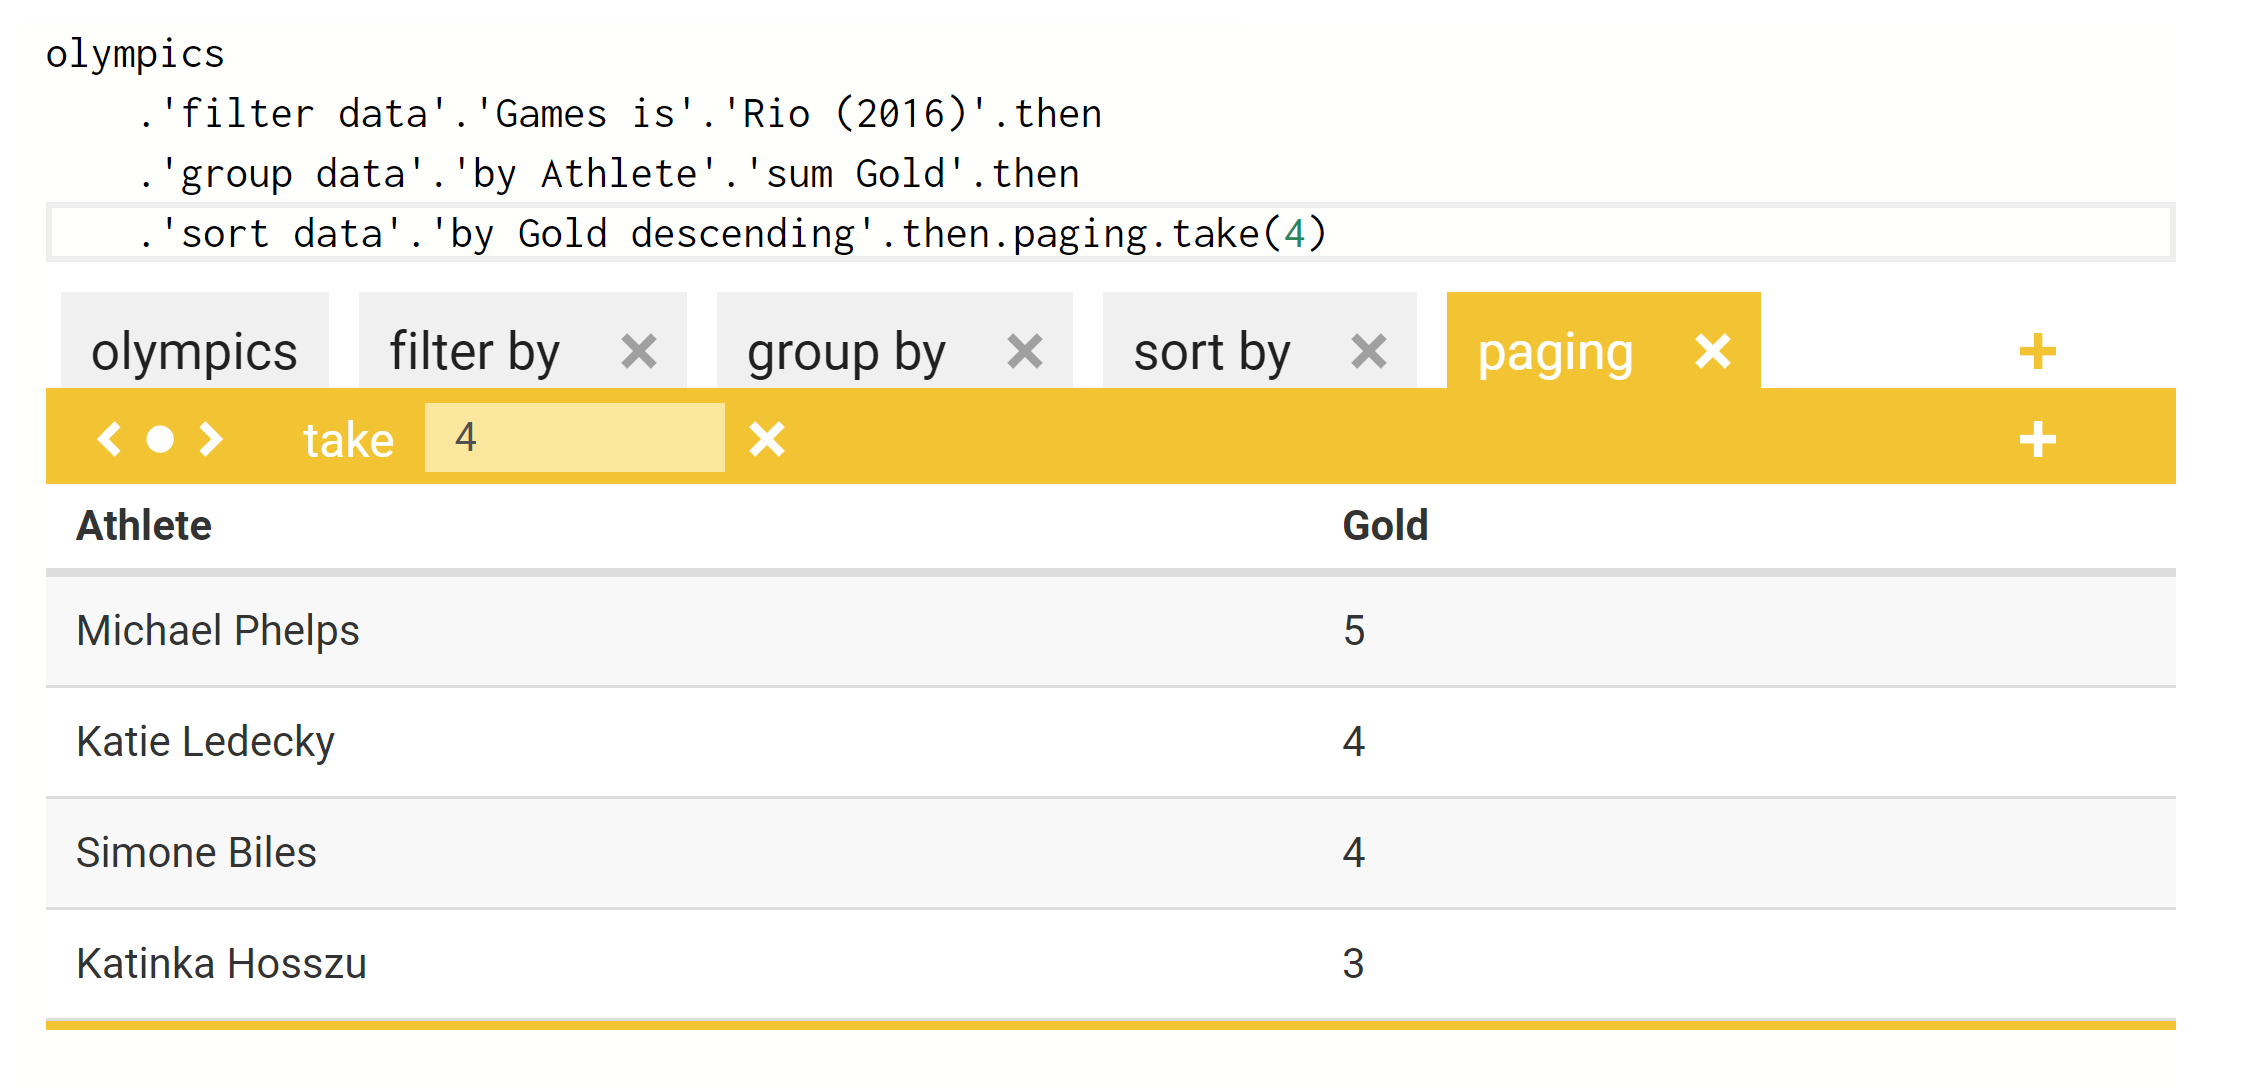
\includegraphics[scale=0.24]{img/live.png}
\caption{A live preview in The Gamma, generated for a code snippet that uses the pivot type
  provider for data exploration. The interface also lets the user navigate through the steps
  of the transformation and modify parameters of the query.}
\label{fig:live}
\end{figure}

~

Finally, the issue of reproducibility has received much attention in the context of notebooks
for data science such as Jupyter \citep{kluyver-2016-jupyter}. Although Jupyter can be used
to produce reproducible notebooks, there are practical barriers to this. In particular, it
allows execution of cells out-of-order, meaning that one can run code in a way that modifies
the global state in an unexpected and non-reproducible way. This has been addressed in multiple
systems \citep{pimentel-2015-noworkflow,koop-2017-dataflow} and our approach in Wrattler builds
on this tradition.

\section{Live data exploration environment}
\label{sec:infra-livedata}

The Gamma explores a particular point in the design space of data exploration
tools. It is built around code written in a simple programming language, leveraging the type
provider introduced in Section~\ref{sec:tp-query}. This focus on code makes it easier to guarantee
reproducibility and transparency of data analyses.  At the same time, the design raises the
question of how easy can data exploration be when done through a text-based programmatic
environment. I revisit this problem from the human-computer interaction perspective in the next
chapter, after discussing the infrastructure that makes using The Gamma easier.

One of the lessons learned from spreadsheets is the value of immediate or live feedback.
To make data exploration in The Gamma easier, the work outlined in this section develops an
efficient method for displaying live previews for The Gamma as illustratd in
Figure~\ref{fig:live}. However, providing live previews in a text-based programming environment
is a challenge \citep{mcdirmid-2007-live}. There are two difficulties:

\begin{nitemize}
\item \emph{Live previews and abstractions.} It is difficult to provide live previews for code
  inside functions or classes, because variables in such context cannot be easily linked to
  concrete values. Even if such abstractions are not used as frequently in data exploration code,
  abstractions are often the key concern in conventional theoretical thinking about programming
  langauge design.

\item \emph{Responding to code changes.} Code in a text editor can change in arbitrary ways and
  so it is unclear how to update existing live preview when an edit is made. This is easier in
  structure editors where edits are limited and understood by the system, but live previews for
  a text-based system need to accommodate large and potentially breaking changes in code.
\end{nitemize}

In the work included as Chapter~\ref{ch:foundations}, I tackle the first challenge by arguing that
we need a better theoretical model of programming languages for data exploration. When data
scientist explore data in a notebook environment, they typically do not introduce new abstractions
and most code is first-order. They often use external libraries, some of which provide higher-order
fucntions (projection, filtering, etc.) and so code may use functions and lambda expressions,
but those are typically passed directly as arguments to those functions. My work thus introduces
the \emph{data exploration calculus}, which is a small formal model of a programming language
that corresponds closely to code written to explore data and can be used to formally study
problems in programmatic data exploration tools.

The problem of responding to code changes is tackled by constructing a dependency graph and
caching its nodes. When the code is edited, the new version is parsed, resulting in a new
abstract syntax tree. The nodes of the tree are then analysed and linked to nodes in a
dependency graph. When the node of the tree corresponds to dependency graph node that has been
created previously (with the same dependencies), the graph node is reused. Live previews are
then computed (and associated with) dependency graph nodes. As a result, when dependencies of
a particular expression do not change, it is linked to the same graph node as before and the
associated live preview is reused.

In the following two sections, I provide a brief review of the data exploration calculus and of
the dependency graph construction mechanism. In Chapter~\ref{ch:foundations}, the data exploration
calculus is then used to formalize the graph construction and show that live previews computed
based on the graph are the same as previews that would be computed by directly evaluating the
data exploration calculus expression. The publication also evaluates the efficiency using live
previews, quantifying the reduction in overhead in contrast to two other evaluation strategies.

\begin{figure}
\raggedright
\hspace{0.5em}{\sffamily Programs, commands, terms, expressions and values}
%
\begin{equation*}
\begin{array}{lcl}
p &\narrow{::=}& c_1; \ldots; c_n\\
c &\narrow{::=}& t\\
  &\narrow{|}& \kvd{let}~x = t~t\\
\end{array}
\qquad
\begin{array}{lcl}
t &\narrow{::=}& o \\
  &\narrow{|}& x\\
  &\narrow{|}& t.m(e, \ldots, e)
\end{array}
\qquad
\begin{array}{lclcl}
e &\narrow{::=}& t &\narrow{|}& \lambda x\rightarrow e\\
v &\narrow{::=}& o &\narrow{|}& \lambda x\rightarrow e\\
\end{array}
\end{equation*}

%
\hspace{0.5em}{\sffamily Evaluation contexts of expressions}
%
\begin{equation*}
\begin{array}{lcl}
C_e[-] &=& C_e[-].m(e_1, \ldots, e_n) ~\lsep~ o.m(v_1, \ldots, v_{m}, C_e[-], e_1,\ldots , e_n) ~\lsep~ -\\
C_c[-] &=& \kvd{let}~x = C_e[-] ~\lsep~ C_e[-]\\
C_p[-] &=& o_1;\; \ldots;\; o_{k};\; C_c[-];\; c_{1};\; \ldots;\; c_n\\
\end{array}
\end{equation*}

%
\hspace{0.5em}{\sffamily Let elimination and member reduction}
%
\begin{equation*}
\begin{array}{l}
\hspace{-0.5em}\begin{array}{l}
o_1;\; \ldots;\; o_{k};\; \kvd{let}~x=o;\; c_{1};\; \ldots; c_n \rightsquigarrow\\
\qquad  o_1;\; \ldots;\; o_{k};\; o; c_{1}[x\leftarrow o];\; \ldots; c_n[x\leftarrow o]\end{array}
~~\text{\small (let)}\\[1.2em]
\inference
  {o.m(v_1, \ldots, v_n) \rightsquigarrow_\epsilon o'}
  {C_p[o.m(v_1, \ldots, v_n)] \rightsquigarrow C_p[o']}
~~\text{\small (external)}
\end{array}
\end{equation*}

\caption{Syntax, contexts and reduction rules of the data exploration calculus}
\label{fig:dec-calculus}
\end{figure}

\subsection{Data exploration calculus}

The data exploration calculus is a small formal language for data exploration. The calculus is
intended as a small realistic model of how are programming languages used in data exploration scripts
and computational notebooks. The calculus itself is not Turing-complete and models first-order
code only, but it supports the notion of external libraries that provide specific data exploration
functionality. This may include standard functions for working with collections or data frames that
are common in Python, but also libraries based on type providers as in the case of The Gamma.

Figure~\ref{fig:dec-calculus} shows the syntax of the calculus.
A program $p$ consists of a sequence of commands $c$.
A command can be either a let binding or a term. Let bindings define variables $x$
that can be used in subsequent commands. As noted earlier, lambda functions can only appear as
arguments in method calls. To model this, the calculus distinguishes between terms that can appear
at the top-level and expressions that can appear as argument in an invocation.
A term $t$ can be a value, variable or a member access, while an expression $e$
can be a lambda function or a term. Values defined by external libraries are written
as $o$.

The evaluation is defined by a small-step reduction $\rightsquigarrow$.
Fully evaluating a program results in an irreducible sequence of
objects $o_1;\; \ldots;\; o_n$ (one object for each command, including let bindings) which can be
displayed as intermediate results of the data analysis. The operational semantics is parameterized
by a relation $\rightsquigarrow_\epsilon$ that models the functionality of external libraries.
Figure~\ref{fig:dec-calculus} defines the reduction rules in terms of $\rightsquigarrow_\epsilon$
and evaluation contexts; $C_e$ specifies left-to-right evaluation of arguments of a method call,
$C_c$ specifies evaluation of a command and $C_p$ defines left-to-right evaluation of a program.
The rule (external) calls a method provided by an external library in a
call-by-value fashion, while (let) substitutes a value of an evaluated variable in
all subsequent commands and leaves the result in the list of commands.

Note that our semantics does not define how $\lambda$ applications are reduced. This is done by
external libraries, which will typically supply functions with arguments using standard $\beta$-reduction.
The result of evaluating an external call is also required to be an object value $o$.
To illustrate how a definition of an external library looks, consider the following script:
%
\begin{equation*}
\begin{array}{l}
\kvd{let}~l = \ident{list}.\ident{range}(\Num{0}, \Num{10})\\
l.\ident{map}(\lambda x \rightarrow \ident{math}.\ident{mul}(x, \Num{10}))
\end{array}
\end{equation*}
%
An external library provides the \ident{list} and \ident{math} objects, as well as
numbers $n$, lists of objects $[o_1, \ldots, o_k]$ and failed computations $\bot$.
Next, the external library needs to define the semantics of the \ident{range}, \ident{mul} and
\ident{map} members through the $\rightsquigarrow_\epsilon$ relation. The following shows
the rules for the \ident{map} operation on lists:
%
\begin{equation*}
\begin{array}{l}
\\[-0.75em]
\inference
  {e[x \leftarrow n_i] \rightsquigarrow o_i \quad (\textit{for all $i\in 1\ldots k$})}
  {[ n_1, \ldots, n_k ].\ident{map}(\lambda x\rightarrow e) \rightsquigarrow_\epsilon [ o_1, \ldots, o_k ]}
\qquad
\inference
  {(\textit{otherwise})}
  {[ n_1, \ldots, n_k ].m(v_1, \ldots, v_n) \rightsquigarrow_\epsilon \bot}
\\[-0.75em]
~
\end{array}
\end{equation*}
%
When evaluating \ident{map}, we apply the provided function to all elements of the list using
standard $\beta$-reduction and return a list of resulting objects. The $\rightsquigarrow_\epsilon$
relation is defined on all member accesses, but non-existent members reduce to the failed
computation $\bot$.

We require that external libraries satisfy two conditions. First, when a method is called with
observationally equivalent values as arguments, it should return the same value (compositionality).
Second, the evaluation of $o.m(v_1,\ldots,v_n)$ should be defined for all $o, n$ and $v_i$ (totality).
The above definition satisfies those requirements by using the standard $\beta$-reduction
for reducing lambda functions and by reducing all invalid calls to the $\bot$ object.
Compositionality implies deterministic behaviour of external libraries and is essential for
implementing an efficient live preview mechanism. The totality of the definition, in turn,
makes it possible to prove the following \emph{normalization} property:
%
\begin{theorem}[Normalization]
\label{thm:normalization}
For all $p$, there exists $n, o_1, \ldots, o_n$ such that $p\rightsquigarrow^{*} o_1;\ldots;o_n$
where $\rightsquigarrow^{*}$ is the reflexive, transitive closure of $\rightsquigarrow$.
\end{theorem}
%
The value of the data exploration calculus is that it can be used to model the functionality
of different tools that support data exploration. The work outlined here (and presented in
full in Chapter~\ref{ch:foundations}) uses the calculus to formalise an efficient mechanism
for showing live previews during the editing of data exploxation script. As mentioned earlier,
the mechanism works by constructing a dependency graph, binding expressions to the graph and
associating live previews with the (cached) nodes of the graph. The formal properties of the data
exploration calculus make it possible to prove that live previews computed in this way are the
same as previews that would be obtained by fully re-evaluating the data exploration script.

\begin{figure}
\vspace{-0.5em}
\centering
\subcaptionbox{
  \raggedright
  Graph constructed from initial expression:
  $\kvd{let}~x = \Num{15}~\kvd{in}~\ident{data.skip}(\Num{10}).\ident{take}(x)$
  \label{fig:dep-graph-a}
}{
  $\xymatrix{
  \bnd{val}(\Num{10}) & \bnd{val}(\Num{15})\\
  \bnd{mem}(\ident{skip},s_0)\ar[d]_{\blbl{arg}(0)} \ar[u]^{\blbl{arg}(1)} &
  \bnd{mem}(\ident{take},s_1)\ar[l]_{\blbl{arg}(0)} \ar[u]_{\blbl{arg}(1)}\\
  \bnd{var}(\ident{data})
  }\qquad$
  \vspace{0.5em}
}
\subcaptionbox{
  \raggedright
  Updated graph after changing $x$ to $10$:
  $\kvd{let}~x = \Num{10}~\kvd{in}~\ident{data.skip}(\Num{10}).\ident{take}(x)$
  \label{fig:dep-graph-b}
}{
  $\xymatrix{
  \bnd{val}(\Num{10})&\\
  \bnd{mem}(\ident{skip}, s_0)\ar[d]_{\blbl{arg}(0)} \ar[u]^{\blbl{arg}(1)} &
  \bnd{mem}(\ident{take}, s_2)\ar[l]_{\blbl{arg}(0)} \ar@/_/[lu]_{\blbl{arg}(1)}\\
  \bnd{var}(\ident{data})
}\qquad$
\vspace{0.5em}
}
\vspace{0.5em}
\caption{Dependency graphs formed by two steps of the live programming process. }
\label{fig:dep-graph}
\end{figure}

\subsection{Computing previews using a dependency graph}

Given a program in the data exploration calculus, I now describe the core of a mechanism that
can be used for providing the user with live previews as illustrated in Figure~\ref{fig:live}.
The key idea behind our method is to maintain a dependency graph with
nodes representing individual operations of the computation that can be evaluated
to obtain a preview. Each time the program text is modified, we parse it afresh (using an
error-recovering parser) and bind the abstract syntax tree to the dependency graph.
When binding a new expression to the graph, we reuse previously created nodes as long as
they have the same structure and the same dependencies. For expressions that have a new
structure, we create new nodes.

The nodes of the graph serve as unique keys into a lookup table containing previously
evaluated parts of the program. When a preview is requested for an expression, we use the graph
node bound to the expression to find a preview. If a preview has not been evaluated, we force
the evaluation of all dependencies in the graph and then evaluate the operation represented by
the current node.


The nodes of the graph represent individual operations of the computation. A node indicates what
kind of operation the computation performs and is linked to its dependencies through edges.
This makes it possible to define computation not just over expressions of the data exploration
calculus, but also over the dependency graph. In order to cache computed previews with the node
as the key, some of the nodes need to be annotated with a unique symbol. That way, we can
create two unique nodes representing, for example, access to a member named \ident{take} which
differ in their dependencies. The graph edges are labelled with labels indicating the kind of
dependency. For a method call, the labels are ``first argument'', ``second argument'' and so on.
Writing $s$ for symbols and $i$ for integers, nodes (vertices) $\bndclr{v}$ and edge labels
$\blblclr{l}$ are defined as:
%
\begin{equation*}
\begin{array}{rcll}
\bndclr{v}&=&\bnd{val}(o) \lsep \bnd{var}(x)\lsep \bnd{mem}(m, s)\lsep \bnd{fun}(x, s)&\qquad(\textit{Vertices})\\
\blblclr{l}&=&\blbl{body} \lsep \blbl{arg}(i)&\qquad(\textit{Edge labels})\\
\end{array}
\end{equation*}
%
The \bnd{val} node represents a primitive value and contains the object itself. Multiple occurrences
of the same value, such as $\Num{10}$, will be represented by the same node. Member access \bnd{mem}
contains the member name, together with a unique symbol $s$ -- two member access nodes with
different dependencies will contain a different symbol. Dependencies of a member access are labelled
with \blbl{arg} indicating the index of the argument ($0$~for the instance and $1,2,3,\ldots$ for the
arguments). Finally, nodes \bnd{fun} and \bnd{var} represent function values and variables
bound by $\lambda$ abstraction.

Figure~\ref{fig:dep-graph} illustrates how to build the
dependency graph. Node representing $\ident{take}(x)$ depends on the argument -- the
number $\Num{15}$ -- and the instance, which is a node representing $\ident{skip}(\Num{10})$.
This, in turn, depends on the instance \ident{data} and the number $\Num{10}$. Note that variables
bound via \kvd{let} binding such as $x$ do not appear as $\bnd{var}$ nodes. The node using it
depends directly on the node representing the expression assigned to $x$.

After changing the value of $x$, we create a new graph. The dependencies of the node
$\bnd{mem}(\ident{skip}, s_0)$ are unchanged. The symbol $s_0$ attached to the node remains
the same and so the previously computed previews can be reused. This part of the program is not recomputed.
The $\blbl{arg}(1)$ dependency of the \ident{take} call
changed and so we create a new node $\bnd{mem}(\ident{skip}, s_2)$ with a fresh symbol $s_2$.
The preview for this node is then computed as needed using the already known values of its
dependencies.

The full description of how the dependency graph is constructed can be found in
Chapter~\ref{ch:foundations}. The construction proceeds recursively over the syntactic structure
of the program in the data exploration calculus. For each expression in the program, it recursively
obtains graph nodes representing its sub-expressions. It then checks the cache to see if a node
representing the current expression with the same dependencies exists already. If so, the node is
reused. If no, a new node (possibly with a new symbol) is created.

The construction of the graph makes it possible to compute preview over the nodes of the
dependency graph and cache the previously computed previews by using the graph node as the cache
key. I illustrate how the evaluation works using two of the reduction rules. For simplicity,
I do not discuss the caching here. I will also write $p$ for evaluated previews which can be either
primitive objects $o$ or functions $\lambda x.e$ (for which we cannot show a preview directly).
Given a dependency graph $(V, E)$ where $V$ is a set of vertices $\bndclr{v_1}, \bndclr{v_2}, \ldots, \bndclr{v_n}$
and $E$ is a set of directed labelled edges of the form $(\bndclr{v_1}, \bndclr{v_2}, \blblclr{l})$,
the evaluation is then defined as a relation $\bndclr{v} \Downarrow p$. The following two rules
illustrate evaluation for primitive values and for member access:
%
\begin{equation*}
\begin{array}{l}
\inference
  {~}
  {\bnd{val}(o) \Downarrow o }~~\text{\small (val)}
\\~\\
\inference
  { \forall i\in\{0\ldots k\}.(\bnd{mem}(m, s), \bndclr{v_i}, \blbl{arg}(i)) \in E \\
    \bndclr{v_i} \Downarrow p_i & p_0.m(p_1, \ldots, p_k) \rightsquigarrow_\epsilon p }
  { \bnd{mem}(m, s) \Downarrow p }~~\text{\small (mem-val)}
\end{array}
\end{equation*}
%
The (val) rule is simple. If a graph node represents a primitive value, it directly reduces to
the value. The (mem-val) rule illustrates a more interesting case. To evaluate a member access,
we need to find the graph nodes that represent its arguments (by looking for links with an
appropriate label), reduce those recursively and then use the external library reduction
$\rightsquigarrow_\epsilon$ to reduce the memeber access.

The sketch presented here omits one interesting aspect of the mechanism. In general, previews
can be provided for all sub-expressions that include variables defined by an earlier let binding.
However, if a sub-expression contains a variable bound by a lambda expression, we have no
way of obtaining suitable value for the variable. In this case, our mechanism evaluates
a delayed preview $\llbracket e \rrbracket_\Gamma$, which represents a partially-evaluated
expression that depends on variables specified by $\Gamma$. Delayed previews could still be
useful if the user interface allowed the user to specify sample value for the free variables
and they also have interesting theoretical connection to work on Contextual Modal Type Theory
\citep{nanevski-2008-cmtt} and comonads~\citep{gabbay-2013-cmtt}.

The full paper, included as Chapter~\ref{ch:foundations}, uses two research methodologies
to evaluate the work. First, it formalizes how the live preview mechanism works using the
model based on the data exploration calculus as sketched above. The formalisation is
used to show that the previews computed over the dependency graph are \emph{correct}. That is,
they are the same as the values we would obtain by evaluating the data exploration calculus
expressions directly. The formalization is also used to list a number of common edits to
a program that do not invalidate previously computed live previews. Examples of such edits
include extracting sub-expression into a let-bound variable, deleting or adding unused code
or changing unrelated parts of the program. The evaluation also employs programming systems
research methods to empirically evaluate the efficiency of the live preview evaluation method.
The paper contrasts the method with standard call-by-value and lazy evaluation strategies
(without caching) and shows the reduction of delays in providing live previews for a sample
coding scenario.

\begin{figure}[t]
\vspace{0.5em}
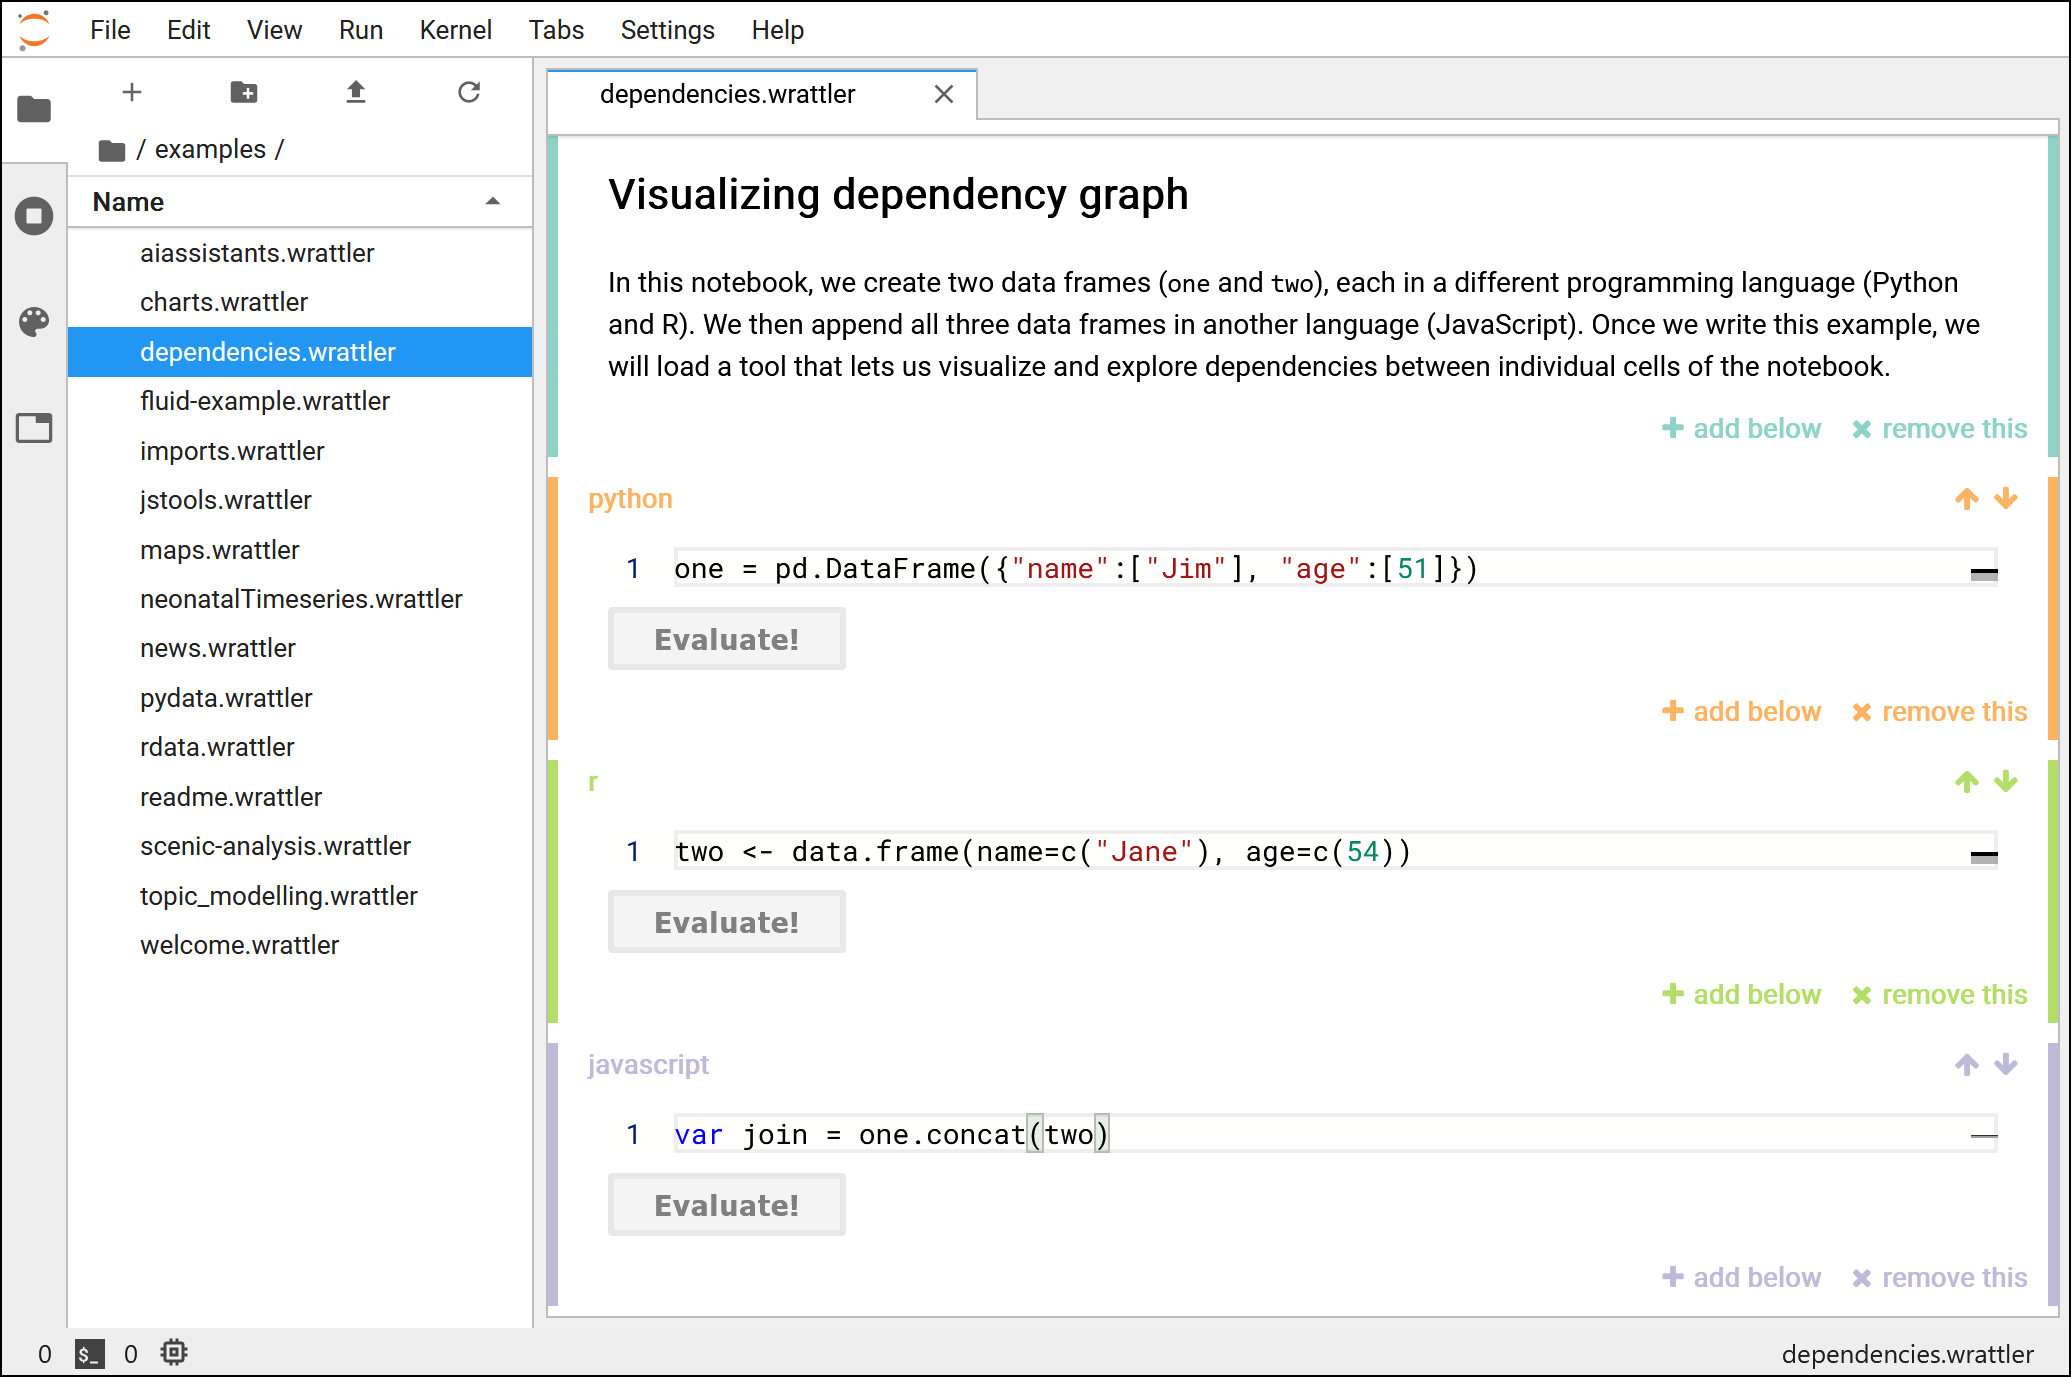
\includegraphics[scale=0.25]{img/wrattler.png}
\caption{Wrattler running inside the JupyterLab system. The opened notebook passes data between
cells written in three different programming languages (Python, R and JavaScript).}
\label{fig:wrattler}
\vspace{0.5em}
\end{figure}

\section{Live, reproducible, polyglot notebooks}

The live data exploration environment discussed in the previous section tackles the problem of
providing rapid feedback to data scientists during data exploration. The other two challenges that
I listed in the opening of this chapter were the need for polyglot tooling support and the need
to make data analyses more reproducible.

The two challenges are addressed by the open-source Wrattler notebook system presented in full in
Chapter~\ref{ch:wrattler}. Wrattler is an extension for the industry standard JupyterLab platform.
As illustrated in Figure~\ref{fig:wrattler}, Wrattler adds a new type of document format that
allows programmers to mix cells written in multiple different programming languages in a single
notebook. The extensibility model of Wrattler makes it possible to support not only new programming
languages, but also interactive tools that run directly in the notebook (hosted in a web browser).
As a result, it is possible to integrate tools that provide live preview mechanism such as
The Gamma and also interactive AI assistants that I discuss in Part~\ref{part:iterative}.
The architecture of the Wrattler system is based on two key principles:

\begin{nitemize}
\item \emph{Polyglot architecture.} The system is designed to allow integration of components in
  different programming languages. This is done by splitting the monolithic architecture of
  Jupyter into individual components including the central data store and multiple language runtimes.

\item \emph{Design for reproducibility.} To guarantee reproducibility and track data provenance,
  the system represents computation as a dependency graph. The graph is similar to the one discussed
  in the previous section, but uses a coarser granularity with one node for each notebook cell.
\end{nitemize}

The Wrattler system is presented in detail in Chapter~\ref{ch:wrattler}. The paper follows the
programming systems methodology. It focuses on the novel system architecture and documents the
capabilities that are enabled by the architecture.

\subsection{Architecture of a novel notebook system}

\begin{figure}[t]
\vspace{0.5em}
\begin{tabular}{p{0.45\textwidth} p{0.55\textwidth}}
\vspace{2em}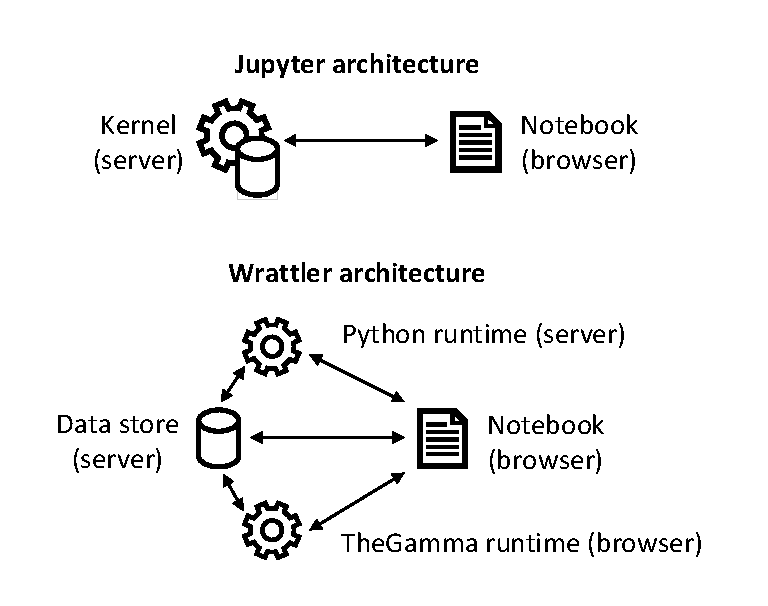
\includegraphics[scale=0.6,trim=1.5cm 6cm 1cm 0.4cm,clip]{img/arch.pdf} &
\vspace{0em}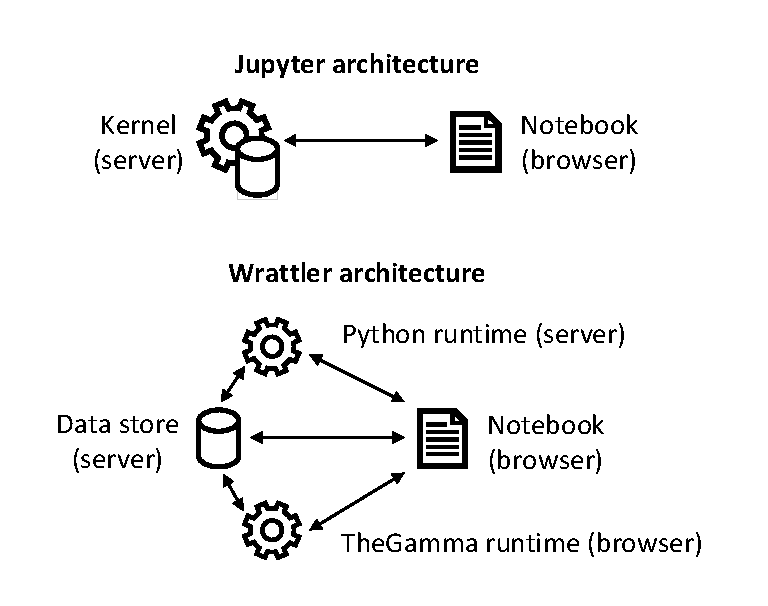
\includegraphics[scale=0.6,trim=1cm 0.5cm 1cm 4cm,clip]{img/arch.pdf}
\end{tabular}
\caption{In notebook systems such as Jupyter, state and execution is managed by a kernel. In
  Wrattler, those functions are split between data store and language runtimes. Language runtimes
  can run on the server-side (e.g.~Python) or client-side (e.g.~The Gamma).}
\label{fig:arch}
\vspace{0.5em}
\end{figure}

Standard notebook architecture consists of a \emph{notebook} and a \emph{kernel}. The kernel
runs on a server, evaluates code snippets and maintains the state they use.
Notebook runs in a browser and sends commands to the kernel in order to evaluate
cells selected by the user. As illustrated in Figure~\ref{fig:arch}, Wrattler splits the
server functionality into two components:

\begin{nitemize}
\item \emph{Data store.} Imported external data and results of running scripts
are stored in the data store. The data store keeps version history and annotates data with
metadata such as types, inferred semantics and provenance information.

\item \emph{Language runtimes.} Code in notebook cells is evaluated by language runtimes.
The runtimes read input data from and write results back to the data store. Wrattler supports
language runtimes that run code on the server (similar to Jupyter), but also browser-based
langauge runtimes.

\item \emph{Notebook.} The notebook is displayed in a web browser and orchestrates
all other components. The browser builds a dependency graph between cells or individual
calls. It invokes language runtimes to evaluate code that has changed,
and reads data from the data store to display results.
\end{nitemize}

The central component of the system is the data store, which enables communication between
individual Wrattler components and provides a persistent data storage.
Data frames stored in the data store are associated with a hash of a node in a dependency
graph constructed from the code in the notebook (using a mechanism discussed below)
and are immutable. When the notebook changes, new nodes with new hashes are created and
appended to the data store. This means that language runtimes can cache data and avoid
fetching them from the data store each time they need to evaluate a code snippet.

External inputs imported into Wrattler notebooks (such as downloaded web pages) are stored as
binary blobs. Data frames are stored in either JSON or binary format.
The data store also supports a mechanism for annotating data frames with
semantic information. Columns can be annotated with primitive data types (date, floating-point
number) and semantic annotation indicating their meaning (address or longitude and latitude).
Columns, rows and individual cells of the data frame can also be annotated with custom metadata
such as their data source or accuracy.

\begin{figure}[t]
\begin{minipage}{.5\textwidth}
\hspace{-1em}
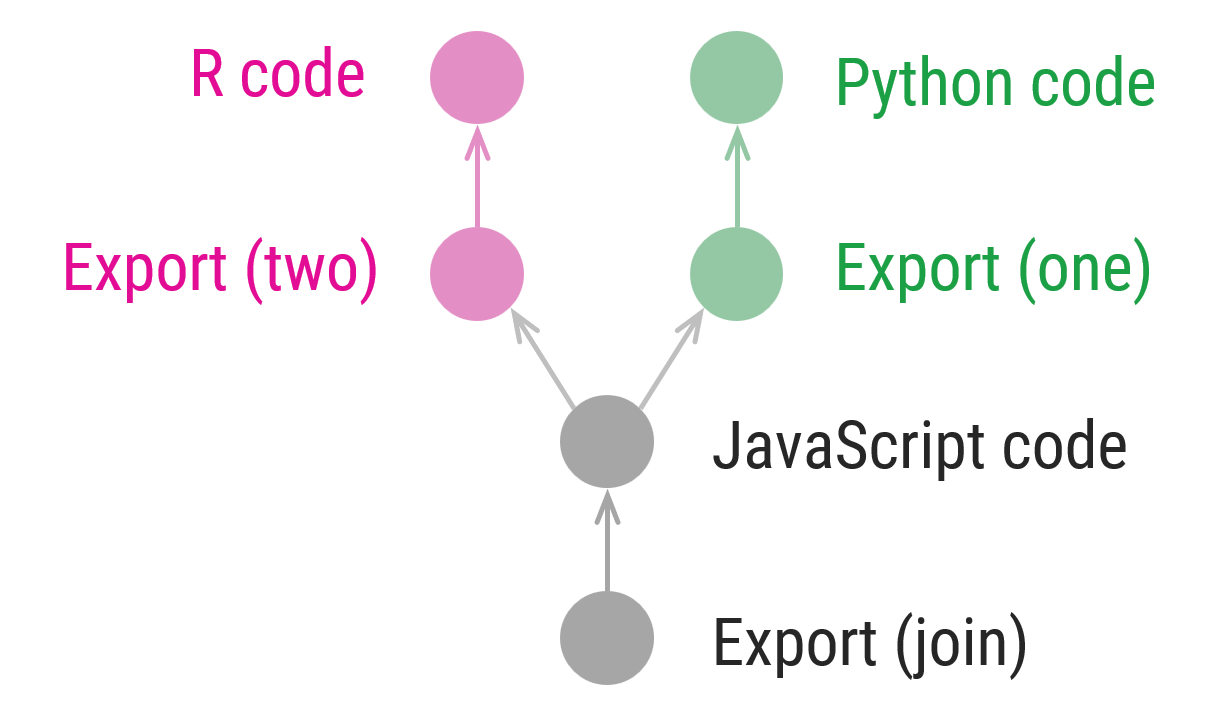
\includegraphics[scale=0.2]{img/graph.png}
\end{minipage}%
\begin{minipage}{0.5\textwidth}
\caption{Dependency graph of a notebook from Figure~\ref{fig:wrattler}. For each cell,
the graph contains a code node and one (or possibly more) export nodes that represent exported
data frames. The R and Python cells are independent and map to independent graph node. The node
corresponding to the final JavaScript cell depends on nodes representing the two variables used
in the code.}
\label{fig:deps}
\end{minipage}
\end{figure}

\subsection{Dependency graphs for notebooks}

At runtime, Wrattler maintains a dependency graph that is remarkably similar to the one
used in the live data exploration environment for The Gamma discussed in
Section~\ref{sec:infra-livedata}. As before, the dependency graph is used to cache results
of previous computations. The nodes in the graph have a unique identifier (hash) that is used
as the key for caching data in the data store. When code in the notebook is modified, the
graph is re-created, reusing previously created nodes where possible.

An example of a dependency graph is shown in Figure~\ref{fig:deps}. For every type of
cell, Wrattler needs to be able to identify the names of imported and exported variables.
In case of Python, R and JavaScript, this is done using a lightweight code analysis.
In case of The Gamma, which can also be used in Wrattler, the full
parse tree and its associated dependency graph is available. A prototype extension of Wrattler
embeds The Gamma graph as a sub-graph of the dependency graph maintained by Wrattler.

An important design choice in the Wrattler design is that cells can only share data in the form
of a data frame. The trade-offs of this choice remain to be evaluated. On the one hand,
it means that Wrattler fits only certain data analytical scenarios. On the other hand, it
makes it possible to easily share data between cells in different languages. In the
example dependency graph, each of the ``export'' nodes thus corresponds to a data frame that
is stored in the data store (using the unique hash of the graph node as the key).

The dependency graph is updated after every code change. This is done using the same
mechanism as in the live data exploration environment discussed in Section~\ref{sec:infra-livedata}.
Wrattler invokes individual langauge runtimes to parse each cell. It then walks over the
resulting structure and constructs nodes for each cell or exported variable with edges
indicating dependencies. The hash for each node is computed from the data in the node (typically
source code or variable name) and hashes of nodes it depends on. An important property of this
process is that, if there is no change in dependencies of a node, the hash of the node
will be the same as before. As a result, previously evaluated values attached to nodes
in the graph are reused.

When the evaluation of an unevaluated cell is requested, Wrattler recursively evaluates all
the nodes that the cell depends on and then evaluates the values exported by the cell.
The evaluation is delegated to a language runtime associated with the language of the node.
For languages that run on the server-side (Python, R), the language runtime sends the source
code, together with its dependencies, to a server that evaluates the code. Note that the
request needs to include only hashes of imported variables as the server can obtain those
directly from the data store. For nodes that run on the client-side (JavaScript, The Gamma),
the evaluation is done directly in the web browser.

\section{Conclusions}

In this chapter, I outlined two contributions to the data analytics infrastructure that
are included in Part~\ref{part:infra} of this thesis. The two contributions describe systems
that aim to make data exploration more live and reproducible, while supporting the polyglot
reality of data processing tools used today.

The work included in Chapter~\ref{ch:foundations} focuses on providing live previews during
data exploration. Can we simplify data exploration by efficiently previewing the result of
a data transformation while the data anlyst is constructing it and tweaking its parameters?
The mechanism presented in this thesis provides a possible answer. The work follows primarily
the programming language research methodology and so it attempts to capture the core idea
behind the appriach, using the simple (but adequate) formal model of the data exploration calculus.
The implementation of the idea provides live previews for code written in The Gamma, a simple
programming language with support for type providers that we encountered already in
Section~\ref{sec:tp-query} and that I will return to once more in the next chapter, but using
the perspective of human-computer interaction research.

The work included in Chapter~\ref{ch:wrattler} presents a polyglot notebook system Wrattler.
The system makes it possible to mix multiple tools in a single notebook. This includes
existing programmatic tools, such as those based on Python and R, as well as novel tools like
The Gamma. The sharing is enabled by the design choice of allowing only data frames as the
exchange format between cells. The promise of the Wrattler architecture is to enable more research
and innovation in the data exploration tooling space. It enables data analysts to use tools they
are already familiar with, but use novel tools where appropriate - for example, include a cell in
The Gamma that will let consumers of their notebooks explore aggregate data without advanced
programming expertise. We will leverage this architecture again in the work on AI assistants
(Chapter~\ref{ch:aia}), outlined in the next chapter.

~

One interesting point that is revealed by putting the two contributions side-by-side is that they
both rely on the same implementation technique. They both maintain a dependency graph of
code (expressions or cells) and update it as the code is edited. The graph is constructed so that
code that remains the same is bound to the same node, making it possible to reuse previously
computed results. The technical similarity is rooted in a broader principle. In both cases,
the reproducible code is the final trace that produces all relevant outputs. The principle is
in contrast with an alternative where code is executed interactively to modify some state
as in systems based on Read-Eval-Print Loop (REPLs).

% ==================================================================================================
% CHAPTER 4: ITERATIVE PROMPTING
% ==================================================================================================

\chapter{Iterative prompting}
\label{ch:iterative}

Data wrangling is the tedious process of getting data into the right format for data exploration.
It involves parsing data, joining multiple datasets, correcting errors and recovering semantic
information. According to domain experts \citep{rattenbury-2017-wrangling}, data wrangling
takes up to 50-80\% of data scientist's time. Unfortunately, there is no easy cure to the problem
of data wrangling. The reason for the difficulty is what \cite{gerrit-2019-csv} refer to
as the \emph{double Anna Karenina principle}: ``every messy dataset is messy in its own way, and
every clean dataset is also clean in its own way.'' In other words, there is no single
characterisation of a clean dataset that tools could optimise for. Human insight into the data
is always needed.

Different research directions approached the problem of data wrangling from different perspectives.
Graphical end-user programming tools typically make it easy to complete the
most common tasks for the most common kinds of datasets, but are incapable of covering the
inevitable special cases that are present due to the double Anna Karenina principle.
Automatic AI-based tools for data wrangling suffer from the same issue. They work well in a
large number of cases, but they can easily confuse interesting outliers for uninteresting
noise in cases where a human would immediately spot the difference. This is perhaps why most
data wrangling is often done manually and often involves a mix of programmatic and end-user
tools. We can make those tools easier to integrate and make tweaking of parameters easier through
live previews (as discussed in the previous chapter), but what if we could offer a different way
of working with them?

The contributions outlined in this chapter are centred around the question of how to
easily enable human data analysts, even if they are not expert programmers, to supply the
necessary human insight to programmatic tools when cleaning and analysing data.
The answer presented in the first contribution (Chapter~\ref{ch:thegamma}) is
an interaction principle that I refer to as \emph{iterative prompting}. In a tool that
follows the principle, the user is repeatedly asked to choose from a list of offered options.
The principle turns the familiar code completion mechanism from a programmer assistance tool
into a non-expert programming mechanism. The two contributions included as Part~\ref{part:iterative}
use iterative prompting in two ways:

\begin{nitemize}
\item In Chapter~\ref{ch:thegamma}, the mechanism is used to allow non-programmers to construct
  data exploration scripts that query data from a range of different data sources. A key
  characteristic of the method is that the mechanism allows users to construct only correct
  scripts and all scripts expressible in the language can be constructed, i.e.,~the principle
  is \emph{correct} and \emph{complete}.

~

\item In Chapter~\ref{ch:aia}, the mechanism is used to guide four different semi-automatic AI data
  wrangling tools. Here, the tools run automatically, but the user can use iterative prompting
  to specify constraints in order to correct errors and oversights in the automatically
  generated solutions. In other words, iterative prompting provides a unified interface through
  which the analyst can supply human insights to the AI tool.
\end{nitemize}

The primary contributions of the work presented in this chapter is that it develops and validates
novel approaches to the problem of data wrangling. To do this, it uses two primary research
methods. The work introducing iterative prompting (Chapter~\ref{ch:thegamma}) is rooted in
human-computer interaction research. It motivates the interaction principle, describes a prototype
implementation and shows its effectiveness through a qualitative case study and an empirical user
study. The work on AI assistants (Chapter~\ref{ch:aia}) combines programming langauge theory and
programming systems research methods. It describes the architecture of the system using a formal
model and validates it by making four existing automatic
AI tools interactive and semi-automatic. The novel tools are evaluated empirically. In cases where
the fully automatic tool fails, our semi-automatic tool allows the user to correct the solution
with a small number (typically 1-2) simple interactions.

The work in this chapter is best seen as design space exploration.
I believe that programming languages and systems provide the right starting point for tackling the
problem of data wrangling and data exploration. But in order to fulfil this role, they need to
be significantly easier to use. Non-programmers need to be able to create simple data exploration
sciprts and data analysts need an easy to use interface for solving typical problems.
Iterative prompting takes the basic auto completion mechanism leveraged by type providers
to a new level, turning it into a simple but powerful unifying sinteraction principle.

\section{Data wrangling and data anlytics}

Data wrangling is most often done manually using a combination of programmatic and graphical tools.
Jupyter and RStudio are popular environments used for programmatic data cleaning.
They are used alongside libraries that implement specific functionality such as parsing CSV files
or merging datasets \cite{gerrit-2019-csv,sutton-2018-datadiff} and general data transformation
functions provided, e.g.,~by Pandas and Tidyverse.\footnote{\url{https://pandas.pydata.org} and
\url{https://www.tidyverse.org} (Accessed 12 June 2024)}

Graphical data wrangling systems such as Trifacta\footnote{\url{https://www.trifacta.com} (Accessed
12 June 2024)} consist of myriad tools for importing and transforming data, which are accessible
through different user interfaces or through a scriptable programmatic interface.
Finally, spreadsheet applications such as Excel and business intelligence tools like Tableau are
often used for manual data editing, reshaping, and especially
visualization \citep{kandel-2011-research}. The above general-purpose systems are frequently
complemented by ad-hoc, for example for parsing PDF documents.

Some of the most practical tools along the entire data wrangling pipeline partially automate
a specific tedious data wrangling task. To merge datasets, Trifacta and datadiff
\citep{sutton-2018-datadiff} find corresponding columns using machine learning. To transform textual
data and tables, Excel employs programming-by-example to parse semistructured
data and many tools exist to semi-automatically detect duplicate records in databases.

~

Interactive and semi-automatic data wrangling tools, allow the analyst to review
the current state of the analysis and make changes to it. The interaction
between a human and a computer in such data wrangling systems follows a number of common patterns:

\begin{nitemize}
\item \emph{Onetime interaction.} A tool makes a best guess, but allows the analyst to manually edit
the proposed data transformation. Examples include dataset merging
in Trifacta and datadiff \citep{sutton-2018-datadiff}.

\item \emph{Live previews.} Environments like Jupyter, Trifacta, and The Gamma
(Chapter~\ref{ch:foundations}) provide live previews, allowing the analyst to check the results and tweak
parameters of the operation they are performing before moving~on.

\item \emph{Iterative.} A tool re-runs inference after each interaction with a human
to refine the result. For example, in Predictive Interaction \citep{heer-2015-predictive}
the analyst repeatedly selects examples to construct a data~transformation.

\item \emph{Question-based.} A system repeatedly asks the human questions about data and uses the
answers to infer and refine a general data model. Examples include data repair tools such as UGuide
\citep{thirumuruganathan-2017-uguide}.
\end{nitemize}

For interactive data wrangling tools, the \emph{live previews} pattern is the most common one
with a varying degree of liveness. Most semi-automatic data wrangling tools accept only
limited forms of human input. The \emph{onetime interaction} pattern is the most common
and only a few systems follow the more flexible \emph{iterative} pattern. The iterative
prompting principle that I introduce in this chapter implements the \emph{iterative} pattern
in a uniform way that is inspired by work on information-rich programming programming
\citep{syme-2013-inforich} and type providers (Chapter~\ref{ch:tp}). It is centred around
code, but reduces the conceptual complexity of coding to a single basic kind of interaction.

\section{Iterative prompting}
Technically speaking, I have already discussed all the components that together make up
the first implementation discussed in this chapter. In The Gamma, the iterative prompting
principle is implemented through the standard code completion mechanism that is
used to select members generated by the type provider outlined in Chapter~\ref{ch:tp}.
The main contribution of the paper included as Chapter~\ref{ch:thegamma} is that it
looks at the design from the perspective of human-computer interaction research.

The key idea behind the principle is that a non-programmer should be able to construct
an entire data exploration script only by selecting appropriate members from a list of
offered choices. Technically speaking, the script thus becomes a single chain of member
accesses. As I discuss below, this also requires a specific type provider design.

The process of data exploration through iterative prompting is illustrated in Figure
Figure~\ref{fig:iterative}, which uses the type provider outlined in Chapter~\ref{ch:tp} to
find the UK House of Lords member from the county of Kent with the most number of days away.
The example shows three steps of the process:

\begin{nenumerate}
\item The user starts by selecting an input data source (not using iterative prompting)
  and types `.' (dot) to see available querying operations. The system offers a list of
  (all available) operations including filtering, grouping and sorting.

\item The user chooses \texttt{filter data}. They are then offered a list of conditions
  based on the columns in the dataset. The user selects \texttt{County is} and is then
  offered a list of all possible values of the column in the dataset. Thanks to the fact
  that iterative prompting in The Gamma is embedded in an ordinary text editor, they
  can start typing to filter the (long) list of possible values.

\item The user chooses \texttt{Kent} as the required value. They are then offered a list
  including further conditons and the \texttt{then} member that makes it possible to choose
  another transformation. They choose \texttt{then} and continue to add sorting.
\end{nenumerate}

\begin{figure}[t]
\hspace{-2em}
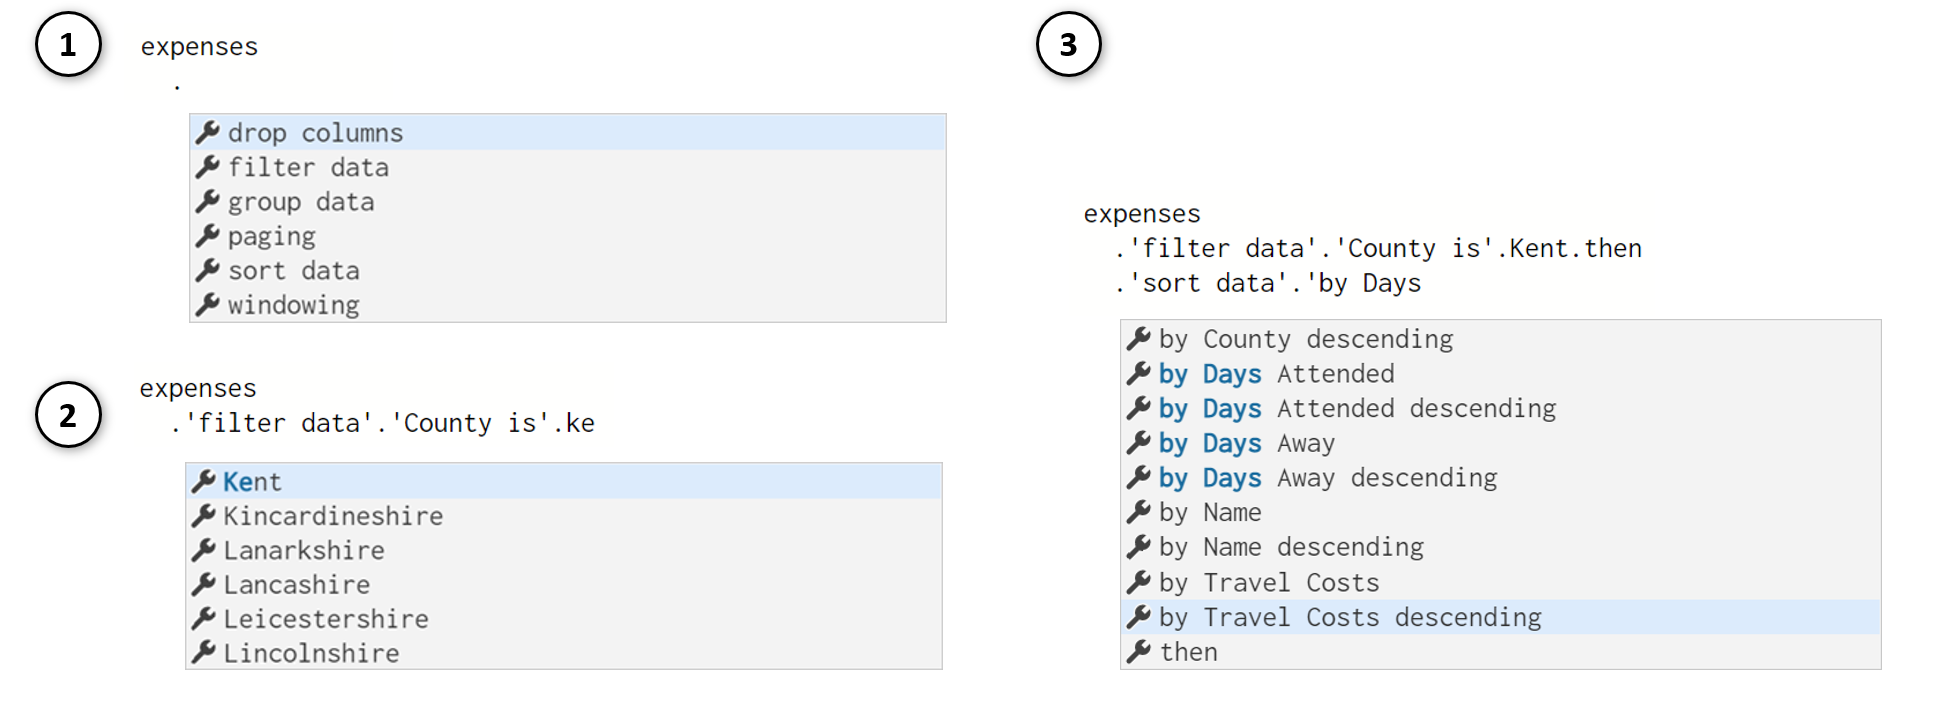
\includegraphics[scale=0.45]{img/iterative.png}
\caption{Using the iterative prompting interaction principle in The Gamma to explore
dataset containing information on UK House of Lords members.}
\label{fig:iterative}
\end{figure}

In The Gamma, the iterative prompting principle is used in the context of text-based
programming language with type providers. This is a deliberate design choice. The aim of the
work is to see whether iterative prompting can make text-based programming accessible to
non-programmers. As a programming language, The Gamma is a simple object-oriented language
with nominal type system and support for type providers. It allows a couple of constructs
in addition to the method chaining shown in Figrue~\ref{fig:iterative} including let binding
and method calls such as \texttt{expenses.paging.take(10)}. I briefly review the design trade-offs
below.

\subsection{Iterative prompting for data querying}

The paper included as Chapter~\ref{ch:thegamma} shows that iterative prompting can
provide a unified interface for exploring data from a range of different data sources.
One of the hypotheses evaluated in the paper is that this aids usability by supporting transfer
of knowledge between different kinds of data sources. To evaluate this, we implemented
type providers for exploring data cubes \citep{syme-2013-inforich}, created by the author of
this thesis, tabular data, as outined in Chapter~\ref{ch:tp} and discussed in
full in Chapter~\ref{ch:dotdriven}, and graph databases.

\begin{figure}[t]
\subcaptionbox{
  \raggedright
  Exploring World Bank data using the data \hspace{20em}
  cube type provider, users choose values from  \hspace{20em}
  two dimensions to obtain a data series.
  \label{fig:cubetp}
}{
  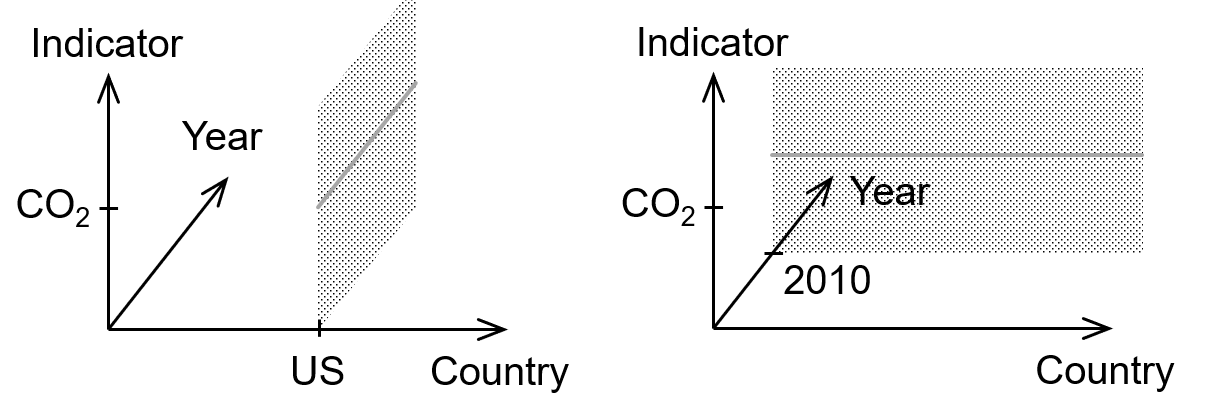
\includegraphics[scale=0.24]{img/cubetp.png}
  \vspace{1em}
}
\quad
\subcaptionbox{
  \raggedright
  To query graph data, the user specifies a path through the data, possibly with
    placeholders to select multiple nodes.  \label{fig:graphtp}
}{
  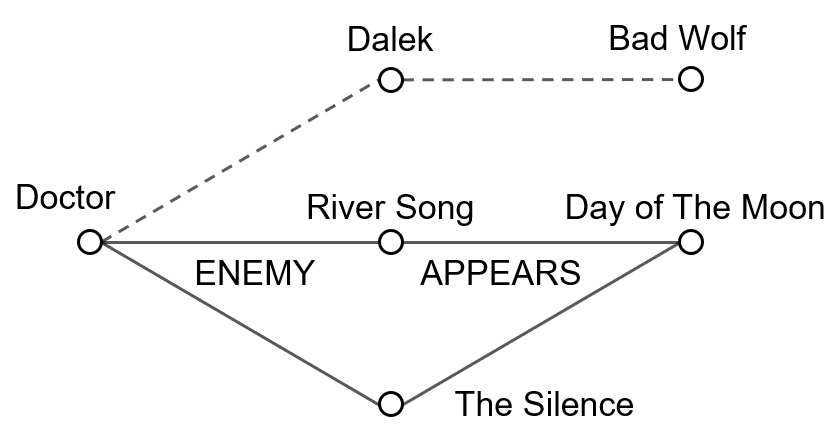
\includegraphics[scale=0.24]{img/graphtp.png}
  \vspace{1em}
}
\vspace{0.5em}
\caption{Design of type providers for exploring cube and graph data}
\label{fig:tpdiags}
\end{figure}

Data cubes are multi-dimensional arrays of values. For example, the World Bank collects
indicators about many countries each year. The type provider makes it possible to select a data
series, such as CO$_2$ emissions of the US over time:

\begin{lstlisting}[language=thegamma]
worldbank.byCountry.'United States'.
  'Climate Change'.'CO2 emissions (kt)'
\end{lstlisting}

\noindent
The dimensions of the \texttt{worldbank} cube are countries, years and indicators.
Figure~\ref{fig:cubetp} illustrates how the provider allows users to slice the data cube --
\texttt{byCountry.\textquotesingle United States\textquotesingle},
restricts the cube to a plane and \texttt{\textquotesingle CO2 emissions (kt)\textquotesingle}
gives a series with years as keys and emissions as values. Similarly, we could first filter the
data by a year or an indicator.

Graph databases store nodes representing entities and relationships between them.
The following example explores a database of Doctor Who characters and episodes. It retrieves
all enemies of the Doctor that appear in the Day of the Moon episode:

\begin{lstlisting}[language=thegamma]
drwho.Character.Doctor.'ENEMY OF'.'[any]'
  .'APPEARED IN'.'Day of the Moon'
\end{lstlisting}

\noindent
The query is illustrated in in Figure~\ref{fig:graphtp}. We start from the \texttt{Doctor} node
and then follow two relationships. We use \texttt{\textquotesingle ENEMY
OF\textquotesingle.\textquotesingle [any]\textquotesingle}
to follow links to all enemies of the Doctor and then specify
\texttt{\textquotesingle APPEARED IN\textquotesingle}
to select only enemies that appear in a specific episode. The members are generated from the data;
\texttt{\textquotesingle ENEMY OF\textquotesingle} and \texttt{\textquotesingle APPEARED IN\textquotesingle} are labels
of relations and \texttt{Doctor} and \texttt{\textquotesingle Day of the Moon\textquotesingle} are labels of nodes. The
\texttt{[any]} member defines a placeholder that can be filled with any node with the specified
relationships. The results returned by the provider is a table of properties of all nodes
along the specified path, which can be further queried and visualized.

Unlike the graph and data cube providers, the type provider for tabular data does not just
allow selecting a subset of the data, but it can be used to construct SQL-like query.
For example, the code constructed in Figure~\ref{fig:iterative} filters and sorts the data.

When using the provider, the user specifies a sequence of operations. Members such as
\texttt{\textquotesingle filter data\textquotesingle} or \texttt{\textquotesingle sort data\textquotesingle}
determine the operation type. Those are followed by members that specify operation parameters.
For example, when filtering data, we first select the column and then choose a desired value.
Unlike SQL, the provider only allows users to choose from pre-defined filtering conditions,
but this is sufficient for constructing a range of practical queries.

\subsection{Usability of iterative prompting}

To evaluate the usability of iterative prompting, we conducted a user study for which we
recruited 13 participants (5 male, 8 female) from a business team of a research institute
working in non-technical roles (project management, communications).
Our primary hypothesis was that non-programmers will be able to use iterative prompting
to explore data, but some aspects of the study were also designed to how users learn to use
the mechanism and whether knowledge can be trasferred between different data sources.
The study methodology and detailed discussion of results can be found in Chapter~\ref{ch:thegamma}.
The key observations from the study are:

\begin{nitemize}
\item \emph{Can non-programmers explore data with The Gamma?}
All participants were able to complete, at least partially, a non-trivial data exploration task and
only half of them required further guidance. A number of participants shared positive comments in
the group interviews. One participant noted that ``this is actually pretty simple to use,''
while another felt the system makes coding more accessible:
``for somebody who does not do coding or programming, this does not feel that daunting.''

\item \emph{How users learn The Gamma?}
There is some evidence that knowledge can be transferred between different data sources. In two
of the tasks, participants were able to complete the work after seeing a demo
of using another data source. One participant ``found it quite easy to translate what you showed
us in the demo to the new dataset.'' Once users understood iterative prompting, they were also
able to learn from just code samples and do not need to see a live demo of using the tool.
One participant noted that ``a video would just be this [i.e.~a code sample] anyway.''

\item \emph{How users understand complex query languages?}
The tabular type provider uses a member \texttt{then} to complete the specification of a
current operation, for example when specifying a list of aggregation operations. Two participants
initially thought that \texttt{then} is used to split a command over multiple lines,
but rejected the idea after experimenting. One participant then correctly concluded that it
``allows us to chain together the operations'' of the query. While iterative prompting
allows users to start exploring new data sources, the structures exposed by more complex data
sources have their own further design principles that the users need to understand.

\item \emph{What would make The Gamma easier to use?}
Three participants struggled to complete a task using the tabular data source,
because they attempted to use an operation that takes a numerical parameter and thus
violates the iterative prompting principle. Most participants had no difficulty navigating
around in text editor and some participants used the text editor effectively, e.g.~leveraging
copy-and-paste. However, two participants struggled with indentation and a syntax error in an
unrelated command. This could likely be alleviated through better error reporting.
\end{nitemize}

\begin{figure}[t]
\centering
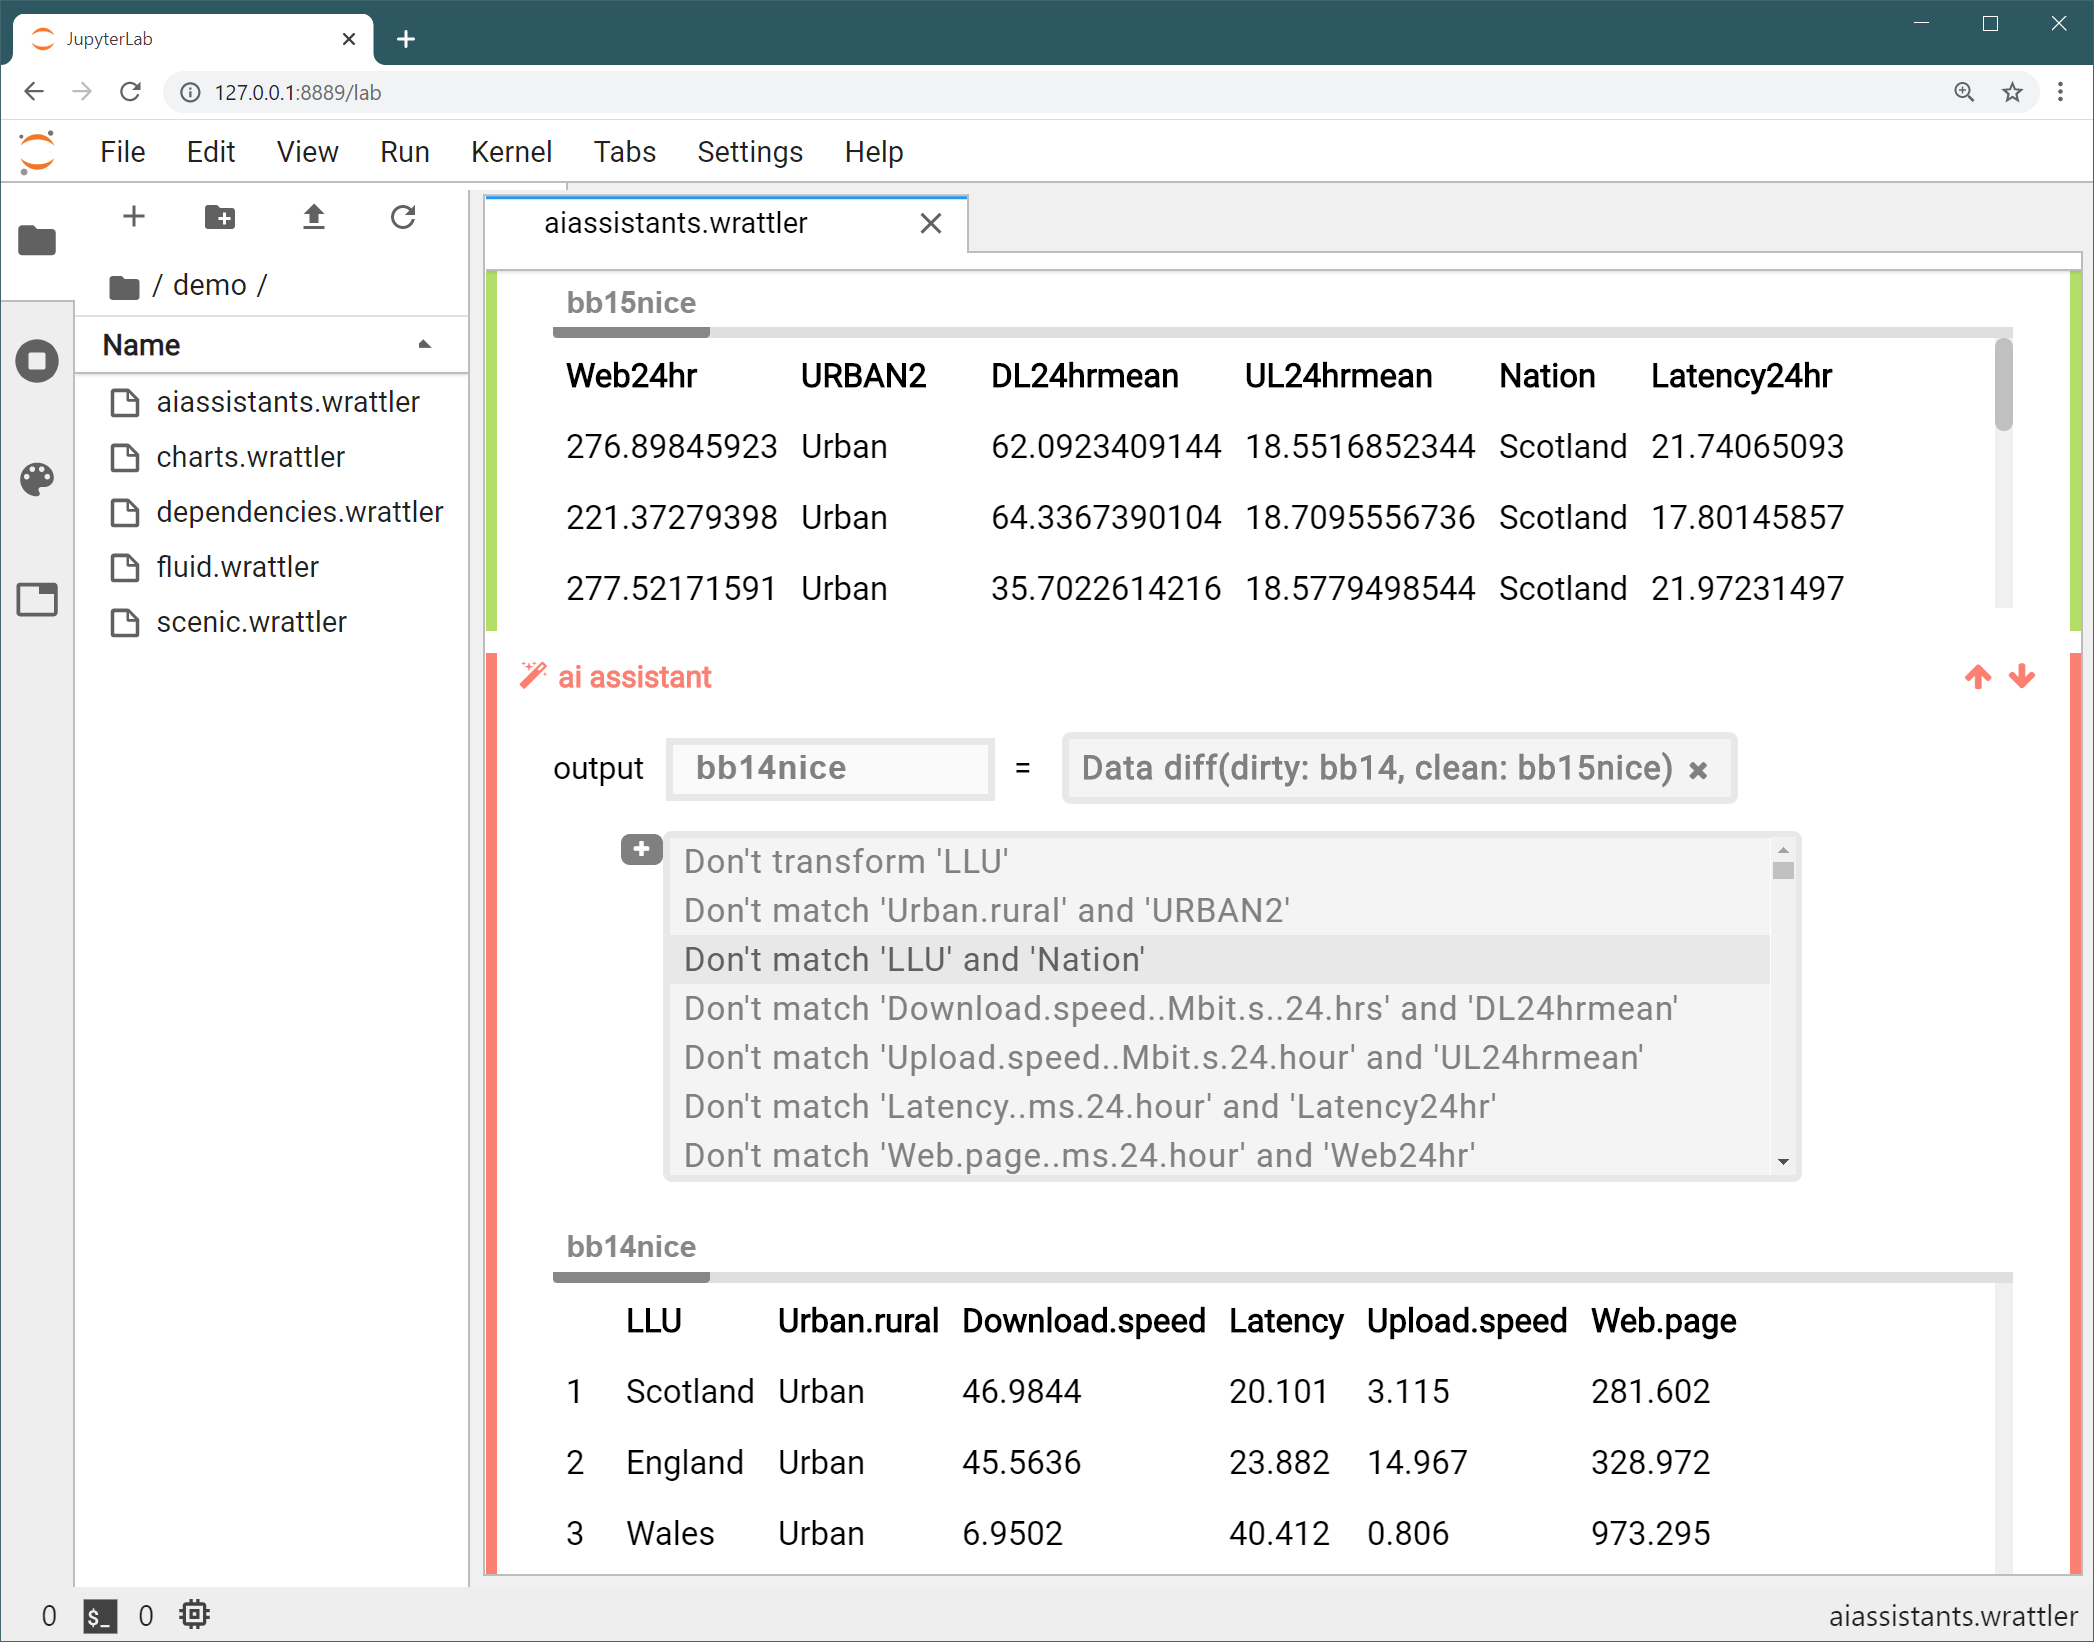
\includegraphics[scale=0.24]{img/datadiff.png}
\caption{Using the datadiff AI assistant inside Wrattler to semi-automatically merge
UK Broadband quality data from two files, parsed by an earlier R script. The user is in the process
of adding a constraint to correct an error in the automatically inferred column matching.}
\label{fig:ddiff}
\end{figure}

\section{AI assistants}
Iterative prompting can be used as a mechanism for program construction, as illustrated in the
previous section, but it can also be used to guide semi-automatic data wrangling tools.
As discussed above, many systems that aim to simplify data wrangling using AI methods support
only the \emph{onetime interaction} pattern where the user invokes the tool and gets back a
result that they can manually refine if needed. In the paper included as Chapter~\ref{ch:aia},
we use iterative prompting as the basis for the AI assistants framework, which is a common
structure for building semi-automatic data wrangling tools that incorporate human feedback.
When using an AI assistant, the user invokes the assistant on some input data, but they can then
repeatedly use iterative prompting to further constrain the solution.

As illustrated in Figure~\ref{fig:ddiff}, AI assistants are available in the
Wrattler notebook system discussed in Chapter~\ref{ch:infra}. In addition to code cells that
obtain, process and visualize data, users can create AI assistant cells that invoke a semi-automatic
data cleaning tool on some of the available datasets. After invoking the assistant, users are
shown a preview of the generated clean dataset. If they see an error in the automatically inferred
solution, they can choose one from the offered options to guide the AI tool and correct the error.
Iterative prompting for AI assistants uses a graphical user interface, but the
interaction mechanism of repeatedly choosing one from the offered options remains the~same.

\subsection{Merging data with Datadiff}

To give an overview of how AI assistants work, consider the task of merging
multiple incompatible datasets, using the UK broadband quality data, published
by the UK communications regulator Ofcom.\footnote{Available at: \url{https://www.ofcom.org.uk/research-and-data/data/opendata}}
The regulator collects data annually, but the formats of the files are inconsistent over the
years. The order of columns changes, some columns are renamed, and new columns are added. We
take the 2014 dataset and select six interesting columns (latency, download and
upload speed, time needed to load a sample page, country, and whether the observation is from
an urban or a rural area). We then want to find corresponding columns in the 2015 dataset.

The 2015 dataset has 66 different columns so finding corresponding columns manually would be
tedious. An alternative is to use the automatic datadiff tool~\citep{sutton-2018-datadiff}, which
matches columns by analyzing the distributions of the data in each column. Datadiff generates a list of
\emph{patches} that reconcile the structure of the two datasets. A patch describes a single data
transformation to, for example, reorder columns or recode a categorical column according to an
inferred mapping. Datadiff is available as an R function that takes two datasets and several
hyperparameters that affect the likelihood of the different types of patches.

When mergning Broadband datasets, datadiff correctly matches five out of six columns, but it
incorrectly attempts to match a column representing Local-loop unbundling (LLU) to a column
representing UK countries. This happens because datadiff allows the recoding of categorical columns,
and seeks to match them based on the relative frequencies in the two columns. Consequently,
the inferred transformation includes a patch to recode the \texttt{Cable}, \texttt{LLU}, and
\texttt{Non-LLU} values to \texttt{Scotland}, \texttt{Wales}, and \texttt{England}. To correct this,
we could manually edit the resulting list of patches, or tweak the likelihood of the
\emph{recode} patch. Such parameter tuning is typical for real-world data wrangling, but finding
the values that give the desired result can be hard.

The semi-automatic datadiff AI assistant presented in this chapter enables the analyst to guide
the inference process by specifying human insights in the form of constraints.
The AI assistant first suggests an initial set of patches with one incorrect mapping. After the
analyst chooses one of the offered constraints, shown in Figure~\ref{fig:ddiff}, datadiff
runs again and presents a new solution that respects the specified constraints
until, after two more simple interactions, it reaches the correct solution.

\subsection{Formal model of AI assistants}

The central contribution presented in Chapter~\ref{ch:aia} is a formal model of AI assistants
that captures their structure. The chapter uses the standard methodology of theoretical
programming language research, but applied to a problem from the data engineering research field.
The definition of an AI assistant captures a common structure that semi-automatic data wrangling
tools can follow in order to use iterative prompting as a mechanism for incorporating human
insights into the data wrangling process.

The formal model defines AI assistants as a mathematical entity that consists of several
operations, modelled as mathematical functions between different sets.
Every AI assistant is defined by three operations that work with expressions~$e$, past human
interactions $H$, input data $\Din$, and output data $\Dout$. Expressions $e$ can also be
thought of as data cleaning scripts. Input and output data are typically one or more data
tables, often annotated with meta-data such as column types.
While AI assistants share a common structure, the language of expressions $e$ that an assistant
produces, the notion of human interactions $H$, and the notion of $\Din$ and $\Dout$ can differ
between assistants.

\begin{definition}[AI assistant]
\label{def:aia}
Given expressions $e$, input data $\Din$, output data $\Dout$, and human interactions $H$, an
\emph{AI assistant} $(H_0, f, \best, \choices)$ is a tuple where
$H_0$ is a set denoting an empty human interaction and
$f, \best$ and $\choices$ are operations such that:
%
\begin{nitemize}
\item $f(e,\Din) = \Dout$
\item $\best_{\Din}(H) = e$
\item $\choices_{\Din}(H) = (H_1,H_2,H_3,\ldots,H_n)$.
\end{nitemize}
\end{definition}

The operation $f$ transforms an input dataset $\Din$ into an output dataset $\Dout$ according to the
expression (data cleaning script) $e$. The operation $\best_{\Din}$ recommends the best expression
for a given input dataset $\Din$, respecting past human interactions $H$. Finally, the operation
$\choices_{\Din}$ generates a sequence of options $H_1, H_2, H_3, \ldots, H_n$ that the
analyst can choose from (e.g.~through the user interface illustrated in Figure~\ref{fig:ddiff}).
When interacting with an assistant, the selected human interaction $H$ is passed back to
$\best_\Din$ in order to refine the recommended expression. Note that the sequence of human
interactions given by $\choices_{\Din}$ may be sorted, starting with the one deemed the most
likely. To initialize this process, the AI assistant defines an empty human interaction $H_0$.

The interesting AI logic can be implemented in either the $\best_\Din$
operation, the $\choices_\Din$ operation, or both. The $f$ operation is typically
straightforward. It merely executes the inferred cleaning script. Both $\best_{\Din}$ and
$\choices_{\Din}$ are parameterized by input data $\Din$, which could be the actual input or a
smaller representative subset to make working with the assistant more efficient.

The working of AI assistants is illustrated in Figure~\ref{fig:interaction}. When using
the assistant, we start with the empty interaction $H_0$. We then iterate until the human analyst
accepts the proposed data transformation. In each iteration, we first invoke $\best_\Din(H)$ to get
the best expression $e^{*}$ respecting the current human insights captured by $H$. We then invoke
$f(e^{*}, \Din)$ to transform the input data $\Din$ according to $e^{*}$ and obtain a transformed
output dataset $\Dout$. After seeing a preview of $\Dout$, the analyst can either accept or reject
the recommended expression $e^{*}$. In the latter case, we generate a list of possible human
interactions $H_1, H_2, H_3, \ldots, H_n$ using $\choices_\Din(H)$ and ask the analyst to pick an
option $H_i$. We use this choice as a new human interaction $H$ and call
the AI assistant again.

The Definition~\ref{def:aia} serves both as a model that can be studied formally,
but also as the basis for an implementation interface of AI assistants. The shared structure
makes it possible to separate the development of individual AI assistants from the development
of tools that use them, such as the AI assistant cell type implemented in Wrattler.

\begin{figure}
\centering
\vspace{-1em}
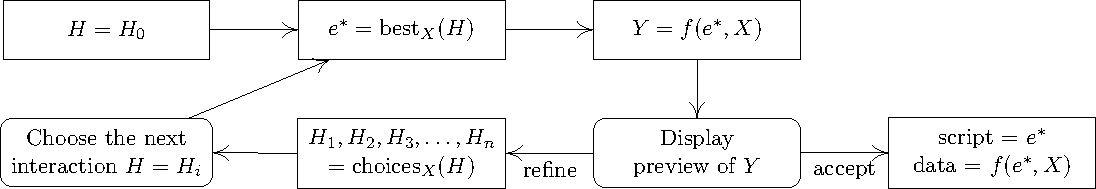
\includegraphics[width=0.95\textwidth]{img/aias.pdf}
\caption{Flowchart illustrating the interaction between an analyst and an AI assistant.
Steps drawn as rounded rectangles correspond to user interactions with the system.}
\label{fig:interaction}
\vspace{-0.5em}
\end{figure}

\subsection{Practical AI assistants}
To show that AI assistants provide a common structure for a wide range of semi-automatic
data wrangling tools, the work included as Chapter~\ref{ch:aia} takes four existing
AI-based data wrangling tools that follow the \emph{onetime interaction} pattern and turns them
into interactive tools that follow the \emph{iterative} pattern. The original tools
cover the entire spectrum of data wrangling ranging from parsing of CSV files~\citep{gerrit-2019-csv}
and merging data files~\citep{sutton-2018-datadiff} to type and semantic information inference
(see Chapter~\ref{ch:aia}).

The approach we use for turning a non-interactive AI tool into an interactive AI assistant
is similar in all four cases. The non-interactive tools generally define an objective function
$Q(e,\Din)$ that scores data cleaning scripts (expressions $e$) based on how well they clean the
specified input data $\Din$. The automatic AI tool performs an optimization, looking for the
best data cleaning from the set of all possible expressions $E$ for the given data. Formally,
the optimization task solved by the existing tools can be written as:
%
\vspace{-0.25em}
\begin{equation*}
\argmax_{e \in E} Q(\Din, e)
\end{equation*}
\vspace{-1.25em}

\noindent
The AI assistants that we implement and formally describe in Chapter~\ref{ch:aia} adapt this
optimization to take account of the human interactions $H$ that have been collected through
the iterative prompting process illustrated in Figure~\ref{fig:interaction}. For a given
human interaction $H$ (starting with $H_0$), we define a set of expressions $E_H$ that is
filtered to only include expressions satisfying the condition specified by the user through
$H$. We also define a parameterized objective function $Q_H$ that is based on the original
$Q$ but increases or decreases the score for certain expressions based on $H$. Given these
two definitions, it is possible to define the $\best_\Din(H)$ operation as solving an
optimization problem:
%
\vspace{-0.25em}
\begin{equation*}
\best_\Din(H) = \argmax_{e \in E_H} Q_H(\Din, e)
\end{equation*}
\vspace{-1.25em}

\noindent
The four concrete AI assistants that we developed use this definition, but they do not
always use human interactions to tweak both $E_H$ and $Q_H$. It is often sufficient to
restrict the set of expressions used by the search and reuse the original unmodified optimization
algorithm. The implementation of the AI assistants (available in Wrattler) generally required
a modification of the underlying non-interactive tool. The modification is tool-specific as
each of the AI assistants is based on a different kind of search algorithm.
%
The four practical AI assistants presented in Chapter~\ref{ch:aia} work as follows:

\begin{nitemize}
\item The \emph{datadiff AI assistant} infers a list of patches that transform the input dataset
  into a format matching that of the given reference dataset. The assistant optimizes score based
  on the similarity of the data distributions of the matched columns. The semi-interactive AI
  assistant allows the user to specify that certain patches (e.g., matching two particular columns)
  should or should not be included in the resulting set.

\item The \emph{CleverCSV AI assistant} infers formatting parameters of a CSV file to optimize a
  metric based on how regular the resulting parsed result is. The semi-interactive AI assistant
  allows the user to specify that a given character should be or should not be used as a delimiter,
  a quote or an escape character.

\item The \emph{ptype AI assistant} infers types of columns in a dataset, detecting outliers and
  values representing missing data. The optimization function looks for a type with maximal
  likelihood based on a probabilistic model. The semi-interactive AI assistant allows the user
  to reject any aspect of the inferred type (type itself, outlier, missing value), effectively
  forcing the search to look for the next most likely type.

\item The \emph{ColNet AI assistant} annotates data with semantic information from a knowledge
  graph such as DBpedia \citep{lehmann-2015-dbpedia}. It uses a Convolutional Neural Network model
  to calculate the score that sampled data is of a given semantic type and then finds the type
  with the greatest score. The semi-interactive AI assistant adapts the scoring, allowing the
  user to specify that a given sample is (or is not) of a specified semantic type.
\end{nitemize}

In Chapter~\ref{ch:aia}, we evaluate the effectiveness of the four AI assistants both qualitatively
and quantiatively. Our qualitative evaluation uses three scenarios in which the different
earlier data wrangling tools are unable to solve a real-world data wrangling challenge using
the \emph{onetime} interaction. We document how the user can use iterative prompting to obtain
the desired result, by repeatedly choosing one option from the offered list. To evaluate
AI assistants quantitatively, we developed a benchmark that counts how many human interactions
are needed to complete a given data wrangling task for multiple datasets (either reusing an
existing benchmark or synthetically generated). The evaluation shows that 1-2 human interactions
are usually sufficient to complete the task.

\section{Conclusions}

This chapter brings together two contributions that aim to reduce the gab between programming
and spreadsheets by making two tasks that typically require some kind of programming easier.
In the first contribution, I focused on data exploration, whereas the second contribution tackles
the task of data wrangling. My work shows that, in both cases, it is possible to solve
a large class of problems using the \emph{iterative prompting} interaction principle where the
user repeatedly chooses one from the offered options. The interaction principle is simple in
that it reduces the cognitive load by using the \emph{recognition over recall} design heuristic.
When using iterative prompting, the users do not need to recall the kind of operation they
could use to solve the problem. Instead they can review the list of offered options and recognize
the most suitable one.

The work included in Chapter~\ref{ch:thegamma} introduces the \emph{iterative prompting}
interaction principle and uses it to view the type provider for data querying outlined in
Chapter~\ref{ch:tp} from a novel perspective using the human-computer interaction research
methodology. Rather than treating auto-completion as a programmer assistance tool, it is
now used as a mechanism that allows non-programmers to construct entire programs. The key
characteristics of the type provider that make this possible is that it is complete and correct,
i.e.~ it makes it possible to construct all programs and any program constructed by
repeatedly choosing one of the offered options is correct (even though some may result in
empty data). The user study that I briefly discussed in this chapter shows that iterative
prompting can be used by non-programmers to complete a range of data exploration tasks
in a code-oriented environment. This suggests that it is possible to combine the reproducibility
and transparency of using code with ease of use approaching that of spreadsheets.

The work included in Chapter~\ref{ch:aia} uses the iterative prompting interaction principle
(albeit without using the term) to provide human insights to semi-automatic data wrangling
tools that I refer to as AI assistants. The challenge addressed by AI assistants is how to
guide data wrangling tools based on AI techniques. Although such tools can solve many problems
automatically, the complexity of real-world data sets often means that some human guidance
is needed. Iterative prompting provides an easy method through which humans can provide such
guidance. The chapter introduces a formal model of AI assistants and uses it as the basis for
the implementation of four practical tools.

The contributions presented in this chapter link together many of the themes and contributions
discussed in earlier chapters. In particular, the notion of type providers was introduced
as a programming tool from the programming language theory perspective in Chapter~\ref{ch:tp}.
This chapter provides an alternative human-centric perspective. The techniques discussed
in Chapter~\ref{ch:infra} make type providers even more usable by providing live previews during
their usage. Finally, the Wrattler notebook system serves as a platform for integrating
many of the experiments discussed in this thesis. For example, it makes it possible to combine
interactive AI assistants with conventional programmatic data exploration using the widely
used Python and R languages.


% ==================================================================================================
% CHAPTER 5: DATA VISUALIZATION
% ==================================================================================================

\chapter{Data visualization}

Data visualization plays a dual role in the data science lifecycle. Quick data
visualizations are needed during data exploration to help data analysts make sense of
data, find errors and understand how their processing scripts work. However, data visualizations
can also be one of the outcomes of data science projects. In particular, data journalists
often analyse data in order to find interesting insights and share those with their readers.
A sophisticated and illuminating data visualization can be a powerful tool for such storytelling.

Producing a quick data visualization during data exploration is usually easy. In programmatic
environments, it is typically a matter of calling a function with a few parameters to specify
the type of chart one wants to see. However, developing a data visualization that helps
the reader gain insight into a complex problem and critically think about it is typically
a challenging programming task.

As an example, consider the interactive data visualization shown in Figure~\ref{fig:youguess},
created using the Compost library discussed below. The visualization is inspired by the New York
Times ``You draw it'' article series \citep{aisch-2015-youdraw}.
It encourages critical thinking by first asking the reader to make a guess
about the actual data. Only after the reader drags the bars according to their presuppositions, the
chart reveals the actual values.

\begin{figure}[h!]
\vspace{1em}
\hspace{-2.5em}
\subcaptionbox{
  \raggedright
  The user first has to guess what the values are
  (here, guess how much the UK government spends per category).
  \label{fig:youguess1}
}{
  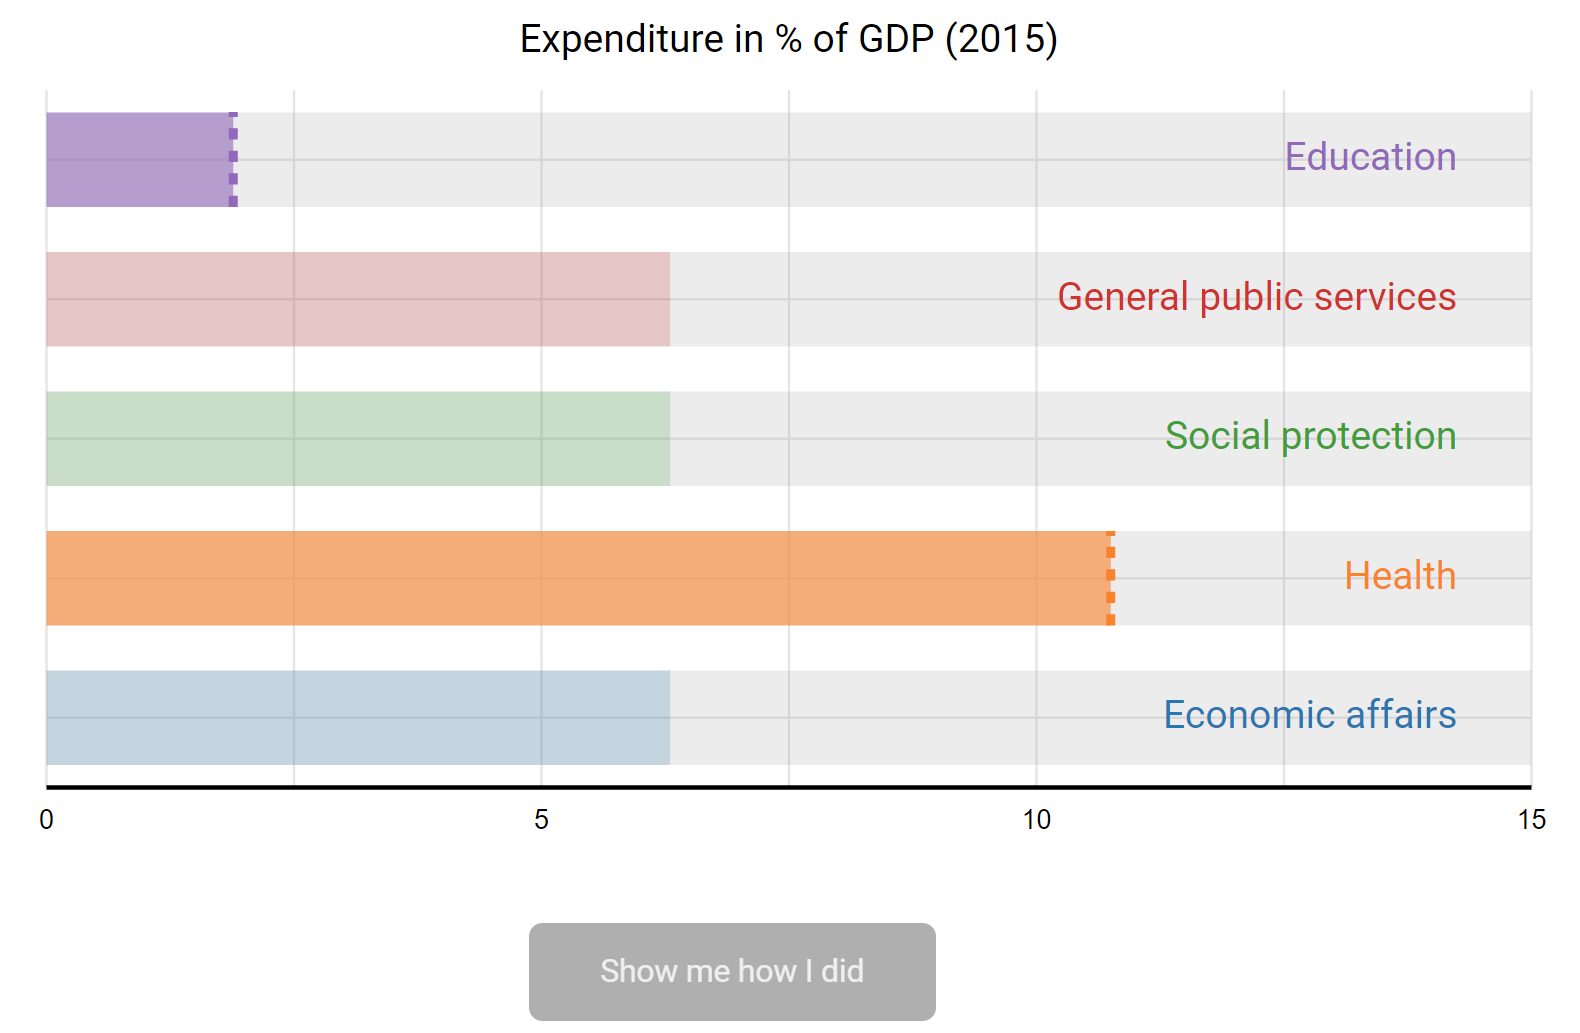
\includegraphics[scale=0.18]{img/youguess1.png}
  \vspace{1em}
}
\quad
\subcaptionbox{
  \raggedright
  After clicking a button, actual data is shown \hspace{10em} (together with a marker showing the guess).
  \label{fig:youguess2}
}{
  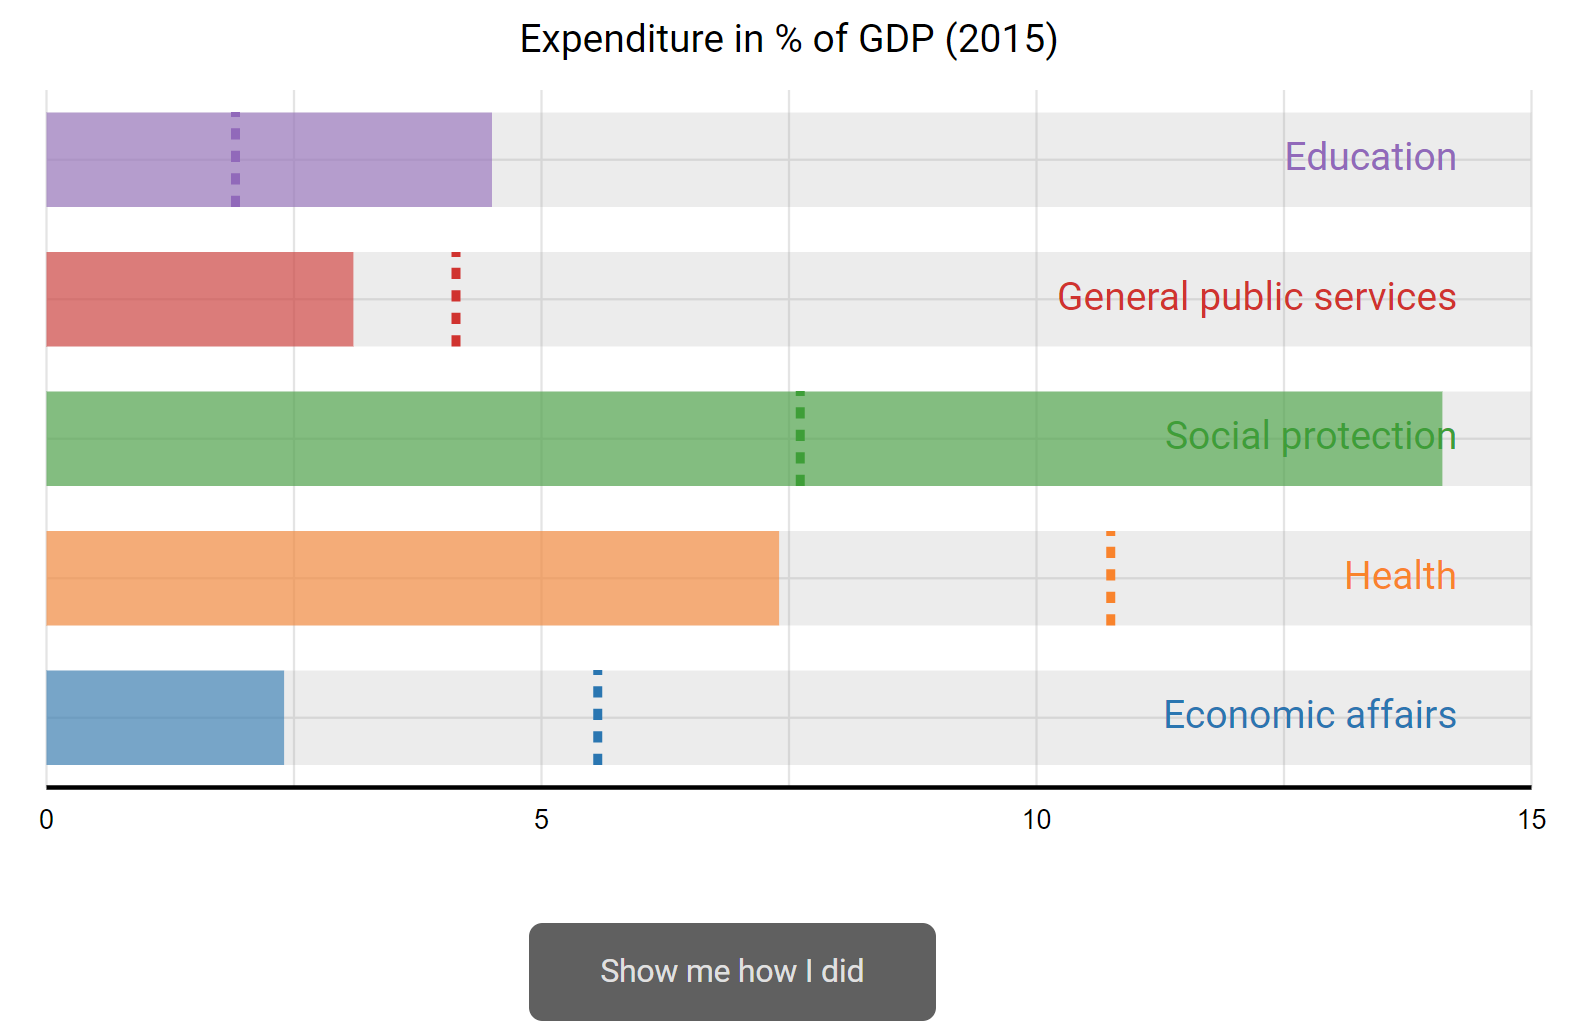
\includegraphics[scale=0.18]{img/youguess2.png}
  \vspace{1em}
}
\vspace{0.5em}
\caption{An interactive data visualization to encourage critical thinking about data created using
the composable Compost data visualization library.}
\label{fig:youguess}
\end{figure}

The chart is based on a standard bar chart, but there are multiple additional aspects that
make creating such chart a challenging programming problem:

\begin{nitemize}
\item The chart combines multiple different visual elements. In additional to the bars themselves,
  it also needs to include the markers (dashed lines) that show the guess.
\item The chart uses a custom color scheme, background to indicate possible area of the bar and it
  grays out the bars for which the user has not yet made a guess.
\item The chart is interactive, allowing the user to drag the end of the bar to any location in
  the specified range (until the button is clicked).
\item Once the button is clicked, a brief animation runs and the bars move from the guessed
  value to the actual value (the marker stays at the original position).
\end{nitemize}

Although numerous charting libraries support some of the above features, creating a custom
data visualization such as the above typically requires using a low-level visualization library
such as D3 \citep{bostock-2011-d3}, which requires advanced programming skills.

More advanced programming skills are needed if one wants to implement data visualizations
that support features such as brushing and linking \citep{buja-1991-linking}. The former allows
the user to focus on a particular region of the chart, while the latter connects two charts and
adapts the visualization in the second chart based on the data selection in the first chart.
Implementing linking is particularly challenging, because it requires understanding what
inputs contributed to the selected data points and then recomputing the data displayed in the
other visualization.

In the following two sections, I provide an overview of two systems that are presented in
Part~\ref{part:visualization}. The sytems make it easier to create rich interactive
visualizations. First, the paper included as Chapter~\ref{ch:compost} presents Compost, a novel
functional data visualization library that makes it possible to compose rich charts
from a small number of primitive building blocks and combinators.
Second, the paper included as Chapter~\ref{ch:galois}
presents a program analysis technique that can be used to automatically create linked data
visualizations based on the code of scritps that construct charts from shared data.
The two systems are aimed at programmers, but they are simple in that they make it possible
to create sophisticated interactive visualizations using small amount of straightforward code.

Both of the papers introduced in this chapter use programming language research methods.
Chapter~\ref{ch:galois} presents the analysis technique formally, using a small model
programming language and discusses its properties. Chapter~\ref{ch:compost} gradually introduces
the concepts of the Compost library in the form of a tutorial. Published as a
functional pearl \citep{gibbons-2010-pearl}, it relies on the tacit assessment of the functional
programming community.

\section{Visualizations to encourage critical thinking}

Data visualizations that aim to present data-driven insights to a broader audience often
require significant programming effort. The ``You draw it'' series by New York Times
\citep{aisch-2015-youdraw} lets the user draw on the chart, while the award-winning visualization
of population density in Asian cities by \cite{bremer-2015-asia} tells a story through multiple
animated and interlinked charts. Visualizations like these are often built using D3
\citep{bostock-2011-d3}, by constructing the chart piece by piece. D3~is easier than drawing
pixels or primitive shapes, but it still requires tediously transforming values to coordinates,
specifying positions in pixels and modifying shape properties in response to events.

Higher-level compositional approaches to chart construction are typically based on grammar of
graphics \citep{wilkinson-1999-grammar}. In grammar of graphics, a chart is a mapping from
data to chart elements and their visual attributes. Libraries based on this idea include
ggplot2 \citep{satyanaran-2016-vega,wickham-2016-ggplot2} and Vega \citep{wickham-2010-layered}.
The mapping is limited to a number of built-in operations, which works well for common types of
scientific charts, but has a limited generality. For example, in Altair~\citep{vanderplas-2018-altair},
it is possible to link multiple charts by specifying a data transformation that relates them,
but this has to be specified using a limited set of combinators provided (and understood) by the
library.

In contrast to systems based on the grammar of graphics, the two systems presented in this chapter
rely on the host programming language to specify the mapping from data to chart elements. A chart
is merely a resulting data type describing the visual elements using domain-specific primitives.
In the two chapters, summarized in the next two sections, we first define a small, orthogonal set
of expressive primitives and then introduce a program analysis technique that can automatically
infer the mapping between source data and elements of the chart.

\begin{figure}[t]
\begin{minipage}[t]{0.6\textwidth}\vspace{-4em}
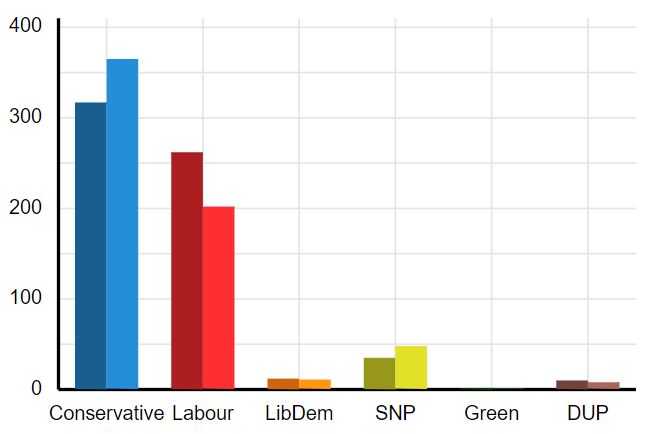
\includegraphics[scale=0.7]{img/compost.png}
\end{minipage}%
\begin{minipage}{0.35\textwidth}\vspace{0pt}
\caption{\raggedright A bar chart that compares the UK general election results
for years 2017 (left) and 2019 (right), created using the Compost library.}
\label{fig:compost}
\end{minipage}
\end{figure}

\section{Composable data visualizations}
The Compost library, presented in Chapter~\ref{ch:compost} can be seen as a functional
domain-specific language for describing charts. As is often the case with domain-specific
languages, finding the right primitives is more of an art than science. The Compost library
is designed in a way that gives it a number of desirable properties:

\begin{nitemize}
\item Concepts such as bar charts, line charts or charts with aligned
  axes are all expressed in terms of more primitive building blocks using a small number of combinators.
\item The primitives are specified in domain terms. When drawing a line, the value of an $y$ coordinate
  is an exchange rate of 1.36 USD/GBP, not 67 pixels from the bottom.
\item Common chart types such as bar charts or line charts can be easily captured as high level
  abstractions, but many interesting custom charts can be created as well.
\item The approach can easily be integrated with the Elm architecture \citep{czaplicki-2016-mvu}
	to create web-based charts that involve animations or interaction with the user.
\end{nitemize}

\subsection{Declarative chart descriptions}

To illustrate the first two points, consider the chart in Figure~\ref{fig:compost}, which
compares UK election results for years 2017 and 2019. In the chart, the $x$ axis shows categorical
values representing the political parties such as ``Conservative'' or ``Labour''. The
$y$ axis shows numerical values representing the number of seats won such as 365 MPs.
When creating a chart, most high-level libraries such as Google Charts expect values in domain
terms, but more flexible libraries like D3 expect the user to first explicitly trnaslate
such domain values to pixels. In Compost, the user composes primitive graphical elements such
as filled rectangles, but their position is specified in terms of domain values.

Our design focuses on two-dimensional charts with $x$ and $y$ axes. Values mapped to those axes
can be either categorical (e.g.~political parties, countries) or continuous
(e.g.~number of votes, exchange rates). The mapping from categorical and continuous values
to positions on the chart, as well as the range of values associated with a scale,
are calculated automatically. Figure~\ref{fig:scales} illustrates the
two kinds of values. A continuous value, written as $\texttt{cont}~n$ contains any number $n$.
A categorical value $\texttt{cat}~c, r$ consists of a categorical value $c$ and a number $r$ between
$0$ and $1$. The second parameter determines an exact position in the range allocated for the
categorical value such as ``Green''.

\begin{figure}[t]
  \vspace{-1em}
  \centering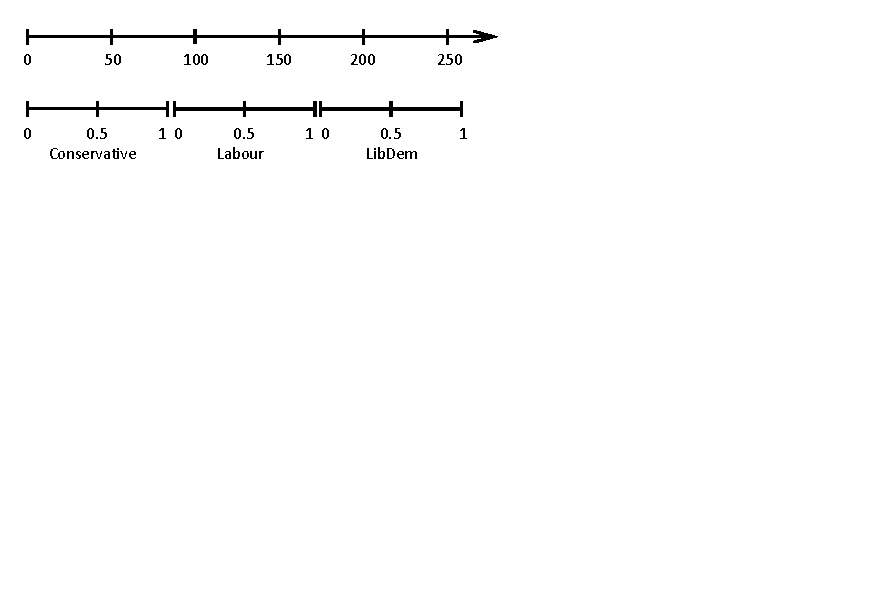
\includegraphics[scale=0.95,trim=0cm 7cm 6cm 0cm,clip]{img/values.pdf}
  \caption{On a continuous scale (above), a position is determined by a number. On a
  categorical scale (below), a position is determined by the category and a number
  between 0 and 1.}
  \label{fig:scales}
\end{figure}

Assuming we have a list \texttt{elections} which contains 5-element tuples with the party name,
colours for 2017 and 2019 and number of MPs for 2017 and 2019, we can construct the chart in
Figure~\ref{fig:compost} as follow (using F\# or similar language with list comprehensions):

\begin{lstlisting}[language=sharp,mathescape=true]
axis$_l$ (axis$_b$ (overlay [
  for party, c17, c19, mp17, mp19 in elections $\rightarrow$
    padding 0, 10, 0, 10, overlay [
      fill clr17, [
        (cat party, 0), (cont 0); (cat party, 0), (cont mp17);
        (cat party, 0.5), (cont mp17); (cat party, 0.5), (cont 0) ],
      fill clr19, [
        (cat party, 0.5), (cont 0); (cat party, 0.5), (cont mp19);
        (cat party, 1), (cont mp19); (cat party, 1), (cont 0) ]
    ]
]))
\end{lstlisting}

\noindent
The central part of the code (lines 4-6 and 7-9) constructs two filled rectangles (bars)
representing number of MPs for 2017 and 2019, respectively. Each rectangle is specified
by four corners (separated using ``;''). The $y$ axist is continuous and the rectangle occupies
space from 0 to the specified number. The $x$ axis is categorical. The first bar takes the
first half of the space available for the party ($0$ to $0.5$) while the second occupies the
second half ($0.5$ to $1$). We then compose the two rectangles using \texttt{overlay}, which
ensures they are rendered on a shared scale. The \texttt{padding} primitive adds a space around
a given shape (specified in pixels). We generate pair of rectangles for each party using a
list comprehension and then overlay all the rectangles before adding axes on the left and bottom.

In addition to the primitives illustrated by the above example, Compost has a number of
other basic shapes (lines, text, bubbles). Perhaps more interestingly, there are also a couple of
combinators that make it possible to combine charts or create charts that share axes.
The \texttt{nest} combinator, explained in Chapter~\ref{ch:compost}, takes a shape (with its own
scales) and nests it inside an explicitly specified range. We can, for example, take a space
defined by a categorical value (from $\texttt{cat}~c, 0$ to $\texttt{cat}~c, 1$) and nest
another shape, or even a line chart, inside this space. In practice, this is useful for combining
multiple charts. The combinator can also apply to one axis only, making it possible to create
two charts that are side-by-side on one axis, but share the other axis.

\subsection{Rendering a Compost chart}

The rendering logic of Compost takes a declarative chart description such as the one generated
by the simple functional program above and transforms it to an SVG in three steps:

\begin{nitemize}
\item \emph{Inferring the scales of a shape}. The implementation first recursively walks over
  the composed shape and infers the ranges of the $x$ and $y$ scales of the shape. For shapes
  constructed using \texttt{overlay}, this unions the ranges of the scales of the contained
  shapes. In case of continuous scale, we take the overall minimum and maximum. For categorical
  scale, the sets of categories obtained for each shape are unioned.

\item \emph{Projecting coordinates}. Once the chart is annotated with the inferred scales, we
  turn all positions from values defined in domain terms to values specified in pixels. This
  is done using a projection function that takes a scale, a space it should be mapped onto
  (in pixels) and a value on the scale. The result are $x$ and $y$ coordinates in pixels.

\item \emph{Rendering chart shapes}. Finally, the recursively defined shape is turned into
  a flat list of shapes in the SVG format. This involves collecting and concatenating
  all the primitive shapes, lines and text elements.
\end{nitemize}

The implementation of the core logic consists of only 800 lines of code. Although the
process is conceptually simple, there is a number of subtle details. In particular,
operations that specify some parameters in pixels (such as padding) have to transform the
projection operation so that the resulting shapes only occupy a space without the specified padding.
Nesting also requires keeping track of the outer range and the inner scale. It is also worth
noting that some operations, such as \texttt{axis} that adds an axis with labels, can be eliminated
at some point in the process. In particular, \texttt{axis} is replaced by overlaid lines and text
elements in the first step.

\subsection{Functional abstraction and interactivity}

As noted earlier, Compost differs from libraries based on the
grammar of graphics such as ggplot2 \citep{wickham-2016-ggplot2} that treat a chart as
as a mapping from data to chart elements and their visual attributes. In Compost,
a chart is a concrete description of chart elements, generated from data by code
written in an ordinary programming language. I illustrated this above with the code that
generated a bar chart using list comprehensions. This means that Compost
can leverage other capabilities of the host~language~and~its~ecosystem.

First, it is possible to easily introduce new higher-level chart abstractions. For example,
the chart shown in Figure~\ref{fig:compost} is sometimes referred to as Dual X-axis Bar Chart.
Some high-level libraries such as Google Charts support this directly. We saw that the
chart can be constructed using Compost, but in a somewhat tedious way. However, in a host
language that lets us define new functions like F\#, we can introduce a new abstraction
for this kind of chart. The following merely extracts the rectangle construction from the
previous example into a function \texttt{dualXBar}:

\begin{lstlisting}[language=sharp,mathescape=true]
let dualXBar xcat clr1 clr2 yval1 yval2 = overlay [
  fill clr1, [ (cat xcat, 0), (cont 0); (cat xcat, 0), (cont yval1);
    (cat xcat, 0.5), (cont yval1); (cat xcat, 0.5), (cont 0) ],
  fill clr2, [ (cat xcat, 0.5), (cont 0); (cat xcat, 0.5), (cont yval2);
    (cat xcat, 1), (cont yval2); (cat xcat, 1), (cont 0) ]
]
\end{lstlisting}

\noindent
We can now use the function inside a list comprehension to construct the original chart
in just three lines of code:

\begin{lstlisting}[language=sharp,mathescape=true]
axis$_l$ (axis$_b$ (overlay [
  for party, c17, c19, mp17, mp19 in elections $\rightarrow$
    dualXBar party c17 c19 mp17 mp19 ]))
\end{lstlisting}

\noindent
One last interesting aspect of the Compost library that is discussed in Chapter~\ref{ch:compost}
is the support for interactivity. The library can be used in conjunction with the
Elm (model-view-update) architecture \citep{czaplicki-2016-mvu} where the programmer defines
the program \emph{state} and \emph{events}. They then provide a function that renders
a chart based on the current state. They also specify a function that updates the sate when
an event occurs. For example, in the earlier interactive chart in Figure~\ref{fig:youguess},
one event is clicking on a bar, which then updates the guessed value. Compost makes programming
such charts easier by reporting events in terms of domain values (using a backward projection).
When user clicks on a bar, the event handler receives a pair of values such as
$\texttt{cat}~\textnormal{``Health''}, 0.3$ and $\texttt{cont}~12.7$. It then updates the
guessed value for the category Health to the new value 12.7\% GDP.

\section{Automatic linking for data visualizations}

The Compost library makes it possible to compose an appealing data visualization from individual
graphical elements. This is necessary if we want to create rich interactive charts. But a single
chart that offers a single perspective is not enough if we want to explain complex data. To
support better understanding, \emph{linked visualizations} \citep{buja-1991-linking}
consist of multiple charts that display different aspects of the same data. When the user
selects an element in one of the charts, the elements that are based on related data as the
selected one are highlighted in the other charts. This makes it possible to relate different
perspectives on the same data.

For example, consider the visualization in Figure~\ref{fig:fluid} that displays data
on energy production over time for different countries and different types of energy.
A single chart with three variables would be difficult to read, so the visualization
instead filters and aggregates the data in two ways. It shows data per country for the year
2015 and ratio of energy produced in the USA and China over time for each type of energy.
The user can select a particular data point (bar on the left, point on the right). If they
select the bar representing the USA, the system infers which input data contributed to the
value (data for all types of energy for the USA in 2015) and computes what chart elements depend
on this data in the second chart (data points for 2015). Selecting Germany
would not highlight any points as the right chart depends only on data points for
China and the USA.

\begin{figure}[t]
  \vspace{-1.5em}
  \hspace{-3.5em}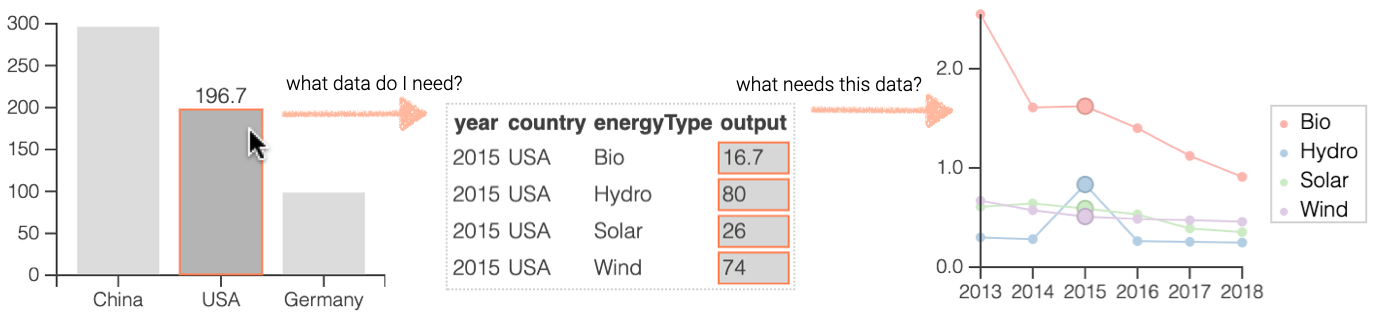
\includegraphics[scale=0.7]{img/fluid.png}
  \caption{Linked data visualization of energy production, showing aggregated data per
  country for 2015 (left) and timeline with the ratio of production
  in the USA and China per energy type (right).}
  \label{fig:fluid}
\end{figure}

Constructing linked visualization like the one in Figure~\ref{fig:fluid} is difficult,
because the data visualization needs to understand how to map selection between the charts.
This can be done automatically for simple data transformations in libraries based on the
grammar of graphics such as Altair~\citep{vanderplas-2018-altair}. In those, simple data
transformations can be expressed using primitives provided by the library. However, the
approach does not work if the data transformation is more complex or if the user prefers to
express it in an ordinary programming language (as ordinary list processing) as opposed to
using a special-purpose domain specific language (grammar of graphics primitives).

In Chapter~\ref{ch:galois}, we use dynamic dependency analysis techniques
to simplify the creation of linked data visualizations. Those techniques have
traditionally been used in areas such as information-flow security, optimisation and
debugging. In our work, we extend the techniques so that they can provide fine-grained
dependency information for programs constructing structured outputs, such as the data structures
used to describe charts in the Compost data visualization library. We introduce a simple
functional programming language Fluid that the users can use to write arbitrary data
transformations and construct charts. By combining two dynamic dependency analyses, we can
then automatically infer the relationships between multiple charts constructed from the
same data.

\subsection{Creating linked visualizations using Fluid}

Consider again the visualization shown in Figure~\ref{fig:fluid}. The two charts are
based on the same input data, which is a collection of records storing the country, energy
type, year and the amount produced. To produce the chart on the left, we filter the data by
year and then sum the produced energy for each of the countries. In Fluid, this is written as
a simple functional program using list comprehensions:
%
\begin{lstlisting}[language=fluid,mathescape=true]
let data2015 =
  [ row | row $\leftarrow$ data, row.year == 2015 ]
let totalFor c =
  sum [ row.output | row $\leftarrow$ data2015, row.country == c ]
let countryData =
  [ { x: c, y: totalFor c } | c $\leftarrow$ ["China", "USA", "Germany"] ]
BarChart { data: countryData }
\end{lstlisting}

The code is similar to what one would write in widely-used functional languages such as
F\# or Haskell. It defines filtered \texttt{data2015}, a helper function \texttt{totalFor}
and then computes data per country using the helper before constructing the resulting chart.
The last step uses a built-in \texttt{BarChart} function. As discussed earlier, this could be
implemented as an abstraction over more basic Compost primitives.

The program analysis automatically infers what values from the source \texttt{data}
contribute to the resulting \texttt{y} value, computed using the \texttt{totalFor} function.
The relevant rows are only those for the year 2015 (due to the filtering) and only those for
the given country (due to the \texttt{totalFor} implementation). It is worth noting that unlike
approaches based on grammar of graphics, we are not restricted to a set of pre-defined primitives.
The data transformation can be arbitrary and we can write it using custom functions such as
\texttt{totalFor}.

The code to construct the second chart is slightly more complicated, because it constructs a
line chart with multiple lines. It defines \texttt{series} helper to obtain a time series for
a given country and energy type, \texttt{plot} helper that calculates ratio between the USA and
China for a given energy type and then composes the chart:
%
\begin{lstlisting}[language=fluid,mathescape=true]
let series type country =
  [ { x: year, y: row.output } | year $\leftarrow$ [2013..2018], row $\leftarrow$ data,
    row.year == year, row.energyType == type, row.country == country ]
let plot type =
  zipWith (fun p1 p2 $\rightarrow$ { x: p1.x, y: p1.y / p2.y })
    (series type "USA") (series type "China")
LineChart { plots: [
  LinePlot { name: type, data: plot type }
    | type $\leftarrow$ ["Bio", "Hydro", "Solar", "Wind"] ] }
\end{lstlisting}
%
The example illustrates two requirements that we have for dynamic dependency analyses that
let us automatically generate linked data visualizations. First, we are not interested in the
resources (code and data) needed to produce the entire result, but only in resources needed to
produce a part of the result. Specifically, if the user clicks on a data point of the line chart,
we want to know what resources contributed to the \texttt{data} field of a specific record in the
list passed to one particular \texttt{LinePlot}. In the analyses, we address this by introducing
the concept of a selection for structured values, which lets us mark a particular part of the
value. (We use this mechanism for analysing charts, but it could equally be used to analyse code
that produces e.g., representations of documents.)

Second, we need multiple different kinds of dependency analyses to automatically link the charts.
If the user selects a part of one chart, we need a \emph{backward} analysis to trace it back to
the original data. This analysis needs to determine parts of the input that were needed for the
output, even if they were also used elsewhere (an alternative analysis would look for inputs
needed only for the particular output).
Then we need a \emph{forward} analysis to determine what outputs it affects in the linked chart.
This, again, needs to determine parts of the output that needed the specific parts of the input,
even if they also needed other umarked inputs (an alternative analysis would look for outputs
that only needed the particular inputs).
As we will see, this analysis leads to four different program analyses.
We use two of them to automatically generate linked data visualizations.

\newcommand*{\evalBwdR}[1]{{\mathrel{\rotatebox[origin=c]{45}{$\Rightarrow$}}}_{#1}}
\newcommand*{\evalFwdR}[1]{{\mathrel{\rotatebox[origin=c]{-45}{$\Rightarrow$}}}_{\hspace{-0.2em}#1}}
\newcommand*{\dual}[1]{{#1}^{\circ}}

\subsection{Language-based foundation for explainable charts}

The program analyses introduced in Chapter~\ref{ch:galois} can be, more broadly, seen as
tools that help us understand how programs work. They could be used to support a range of
use cases outside of the narrow domain of data visualization. However, to keep the presentation
simpler, I will focus on this particular use case. Given the scope of the Fluid language
and the considerable number of analyses, I do not discuss many details in this overview
and focus on sketching the overall structure of the analyses and their key properties.

The analyses are built around the central notion of a program trace $T$. The traces
are generated during program evaluation and they collect information about how the
evaluation proceeded. More formally, a trace is a compact representation of the derivation
trees in the operational semantics. Given a program $e$ and a variable environment $\rho$,
the following judgement states that the program reduces to a value $v$, producing a trace $T$:
%
\begin{equation*}
T :: \rho, e \Rightarrow v
\end{equation*}
%
The program analyses operate on values where some parts are marked as selected. For example,
if a program $e$ produces a value $v$ that represents a chart using the primitives of the Compost
library, we can mark some parts of the resulting chart, for example a bar created using the
\texttt{fill} primitive.

Formally, we annotate values and terms with selection states $\alpha$ from a bounded
lattice of selections $\mathcal{A}$. It is possible to annotate primitive values such as
numbers $n_\alpha$ or empty lists $\textnormal{\texttt{[]}}_\alpha$ but also values that
contain further values such as a non-empty list (a cons cell) such as
$v_1\, \textnormal{\textbf{:}}_\alpha\, v_2$. This would indicate that we are interested in
data that determined that the list will be non-empty (but not the specfic values it contains).
In practice, the most useful kind of annotation is a two-point lattice (selected, non-selected),
but the generality allows for other uses, such as a vector of selections (to be computed in one
step and displayed using different colours).

\subsection{Bidirectional dependency analyses}

The program analyses that are introduced in Chapter~\ref{ch:galois} are defined for a fixed
computation $T :: \rho, e \Rightarrow v$ where $T$ is the trace. In practice, the system evaluates
the expression $e$ and uses the resulting trace $T$ repeatedly for different analyses and
with multiple possible selections. The first two analyses that we define are the backward and
forward data dependency analyses written as $\evalFwdR{T}$ and $\evalBwdR{T}$, respectively.
The two analyses are defined over the trace $T$ and take the availability-annotated
variable context and an expression $\rho, e$ as inputs. They produce an annotated value
$v$, which is the same as the value computed initially, but with availability annotations.
Their intuitive meaning is as follows:

\begin{nitemize}
\item \emph{Forward data dependency} $\rho, e, \alpha\; \evalFwdR{T}\; v$ or \emph{``what only needs me''}.
  Given a context and expression where annotations indicate what resources (data and parts of
  the program) are available, the analysis produces a value with annotations indicating what
  part of the value can be computed using only the available resources.
\item\emph{Backward data dependency} $\rho, e, \alpha\; \evalBwdR{T}\; v$ or \emph{``what do I need''}.
  Given an annotated value $v$, the analysis follows the evaluation backwards (using the trace
  $T$) and annotates resources (data and parts of the program) that have to be available in
  order to produce the annotated parts of the value $v$.
\end{nitemize}

The two analyses form a Galois connection, i.e., the two analyses are not exactly inverses,
because they approximate in some ways, but they are close. For example, if we have a value with
a selection $v$, ask what is needed for the selection using $\evalBwdR{T}$ and then ask
what can be computed using the same data using $\evalFwdR{T}$, we may find that other parts of
the value can also be computed, but the original selection will certainly also be included.

Interestingly, the forward and backward data dependency analyses are not sufficient to
support linked data visualizations. The backward analysis can correctly determine what parts of
the input are needed in order to produce the selected output. However, to highlight the related
elements of the other chart, we do not need to know what the input selection is \emph{sufficient}
for, but what it is \emph{necessary} for. In other words, we do not need to know what can be
computed using only the selected parts of the input, but what part of the result will they
certainly contribute to. This can be formulated as a dual of the original analyses. What would we
not be able to compute if the selected data were unavailable?

In the paper included as Chapter~\ref{ch:galois}, we define this duality formally and exploit
it to define De Morgan dual $(\dual{\evalFwdR{T}}, \dual{\evalBwdR{T}})$ of the Galois
connection $(\evalBwdR{T}, \evalFwdR{T})$, which itself also forms a Galois connection.
The intuitive meaning of the new analyses is as follows:

\begin{nitemize}
\item \emph{Dual forward data dependency} $\rho, e, \alpha\; \dual{\evalFwdR{T}}\; v$ or \emph{``what needs me''}.
  For an annotated context and expression (resources), the analysis highlights what
  parts of the resulting value depend on the specified resources, i.e., what would we not be
  able to compute if the selected parts of the value were unavailbale.
\item \emph{Dual backward data dependency} $\rho, e, \alpha\; \dual{\evalBwdR{T}}\; v$ \emph{``what do only I need''}.
  Given an annotated value, the analysis highlights parts of the program and data
  that are only needed for producing the selected output, i.e., resources that
  would not be needed if the selected part of the output was not needed.
\end{nitemize}

In order to construct a linked data visualization, we need to combine two of the data analyses.
When the user selects a part of one chart, we annotate the relevant part of the structured value
that represents the chart with a selection $\alpha \in \mathcal{A}$ that marks the part.
We then use the backward data dependency analysis $\evalBwdR{T}$ to compute what resources are needed
for producing the output. To mark corresponding parts of another chart, we then use the
dual forward dependency analysis $\dual{\evalFwdR{T}}$. This marks parts of the other chart
that depend on the resources needed for the first chart.

\section{Conclusions}
In this chapter, I provided an overview of the contributions to data visualization included in
Part~\ref{part:visualization}. The focus of this work has been on simplifying the construction
of rich interactive charts that assist the viewer gain deeper insight into the presented data.
While producing simple charts is often easy, building a visualization that combines custom
visual elements, interactivity and allows linking multiple charts requires advanced programming
skills. Unlike with the work outlined in Chapter~\ref{ch:iterative}, I do not hope that the work
presented here will allow non-programmers to create rich interactive data visualizations.
However, Compost and Fluid show that programming data visualizations that encourage critical
thinking about data can be significantly easier than using systems that are widely used today.

The two contributions presented in this chapter also serve as a good justification for using
programming language research methods in the context of tools for data science. In particular,
the work included as Chapter~\ref{ch:compost} relies on the minimalist design of highly composable
functional (domain-specific) languages. It presents the Compost charting library, which lets
programmers compose charts by combining a small number of primitives (such as a filled shape
or a text) using a small number of combinators (overlaying, nesting of scales). The library is
simple to use mainly due to the fact that all positions are specified in terms of domain units
on a continuous numerical scale or a categorical scale (with 0 to 1 range for each category).

The work included as Chapter~\ref{ch:galois} uses dynamic program analysis techniques to
automatically create linked data visualization where the user can explore relationships between
data in multiple charts. The system works by analysing the program that is used to construct the
chart from source data (by filtering and aggregating it in various ways). When the user clicks on
an element of a chart, the system uses two different dynamic dependency analysis techniques to
higlight elements of other charts that depend on the same data as the element selected by the user.
The Chapter~\ref{ch:galois} uses methods of programming language theory to describe the mechanism.
We formalize the programming language, define two analyses, derive their duals, and describe their
formal properties.

Although the prototype implementation of the two systems is not currently integrated, the
two contributions presented in this chapter are closely related. In particular, the program
analysis techniques developed for Fluid would combine well with a composable data visualization
library like Compost.

In this chapter, I also completed one loop of the data science lifecycle illustrated in
Figure~\ref{fig:lifecycle}. The loop started with data acquisition using type providers,
continued with data cleaning and exploring using novel notebook systems and iterative prompting
and now concludes with data visualization. This is the last step in an exploratory phase of
the data science lifecycle where the aim is to understand and explain interesting aspects of data.
An illuminating data visualization that conveys interesting insights found in data is often
the end goal of the process. The production phase that aims to turn the result of the data
analysis into a running component of a larger system is perhaps equally interesting, but
is out of scope for this thesis.

% ==================================================================================================
% PART II - V: PAPERS
% ==================================================================================================

\nobibliography*

\part{Publications: Type providers}
\label{part:providers}

\chapter{Types from data: Making structured data first-class citizens in F\#}
\label{ch:fsdata}

\bibentry{petricek-2016-data}

\chapter{Data exploration through dot-driven development}
\label{ch:dotdriven}

\bibentry{petricek-2017-dot}

\part{Publications: Data infrastructure}
\label{part:infra}

\chapter{Foundations of a live data exploration environment}
\label{ch:foundations}

\bibentry{petricek-2020-live}

\chapter{Wrattler: Reproducible, live and polyglot notebooks}
\label{ch:wrattler}

Tomas Petricek, James Geddes, and Charles Sutton. 2018. Wrattler: Reproducible, live and
polyglot notebooks. In \emph{10th USENIX Workshop on the Theory and Practice of Provenance,
TaPP 2018, London, UK, July 11-12}, 2018, Melanie Herschel (Ed.). USENIX Association.

% this does not work, no idea why
\bibentry{petricek-2018-notebooks}

\part{Publications: Iterative prompting}
\label{part:iterative}

\chapter{The Gamma: Programmatic data exploration for non-programmers}
\label{ch:thegamma}

\bibentry{petricek-2022-gamma}

\chapter{AI Assistants: A framework for semi-automated data wrangling}
\label{ch:aia}

\bibentry{petricek-2023-aia}

\part{Publications: Data visualization}
\label{part:visualization}

\chapter{Composable data visualizations}
\label{ch:compost}

\bibentry{petricek-2021-compost}

\chapter{Linked visualisations via Galois dependencies}
\label{ch:galois}

\bibentry{petricek-2022-galois}

% ==================================================================================================
% PART VI: CONCLUSIONS
% ==================================================================================================

\part{Conclusions}

\chapter*{Contributions}
\label{ch:contribs}
\addcontentsline{toc}{chapter}{\nameref{ch:contribs}}

The contributions presented in this thesis is the result of my long-term effort to
rethink data science tooling from the perspective of programming languages research.
The work has been undertaken at multiple institutions (Microsoft Research, The Alan
Turning Institute, University of Kent) and involved collaboration with a number of
co-authors. The following summarizes my contribution. With the exception of
Chapter~\ref{ch:galois} \citep{petricek-2022-galois},
I am the first author of the included papers.

\begin{nitemize}
\item Chapter~\ref{ch:fsdata} \citep{petricek-2016-data} -- I developed the initial version
  of the library, developed the formal model and wrote most of the paper. Gustavo Guerra significantly
  improved the initial implementation. Don Syme first developed the CSV type provider, assistend with
  the formalization and provided the problem framing.
\item Chapter~\ref{ch:dotdriven} \citep{petricek-2017-dot} -- I am the sole author of the paper,
  but some aspects of the work have benefited from discussion with Don Syme.
\item Chapter~\ref{ch:foundations} \citep{petricek-2020-live} -- I am the sole author of the paper,
  but the work has benefited from discussions with Dominic Orchard, Stephen Kell, Roly Perera and
  Jonathan Edwards and detailed feedback from Dominic Orchard.
\item Chapter~\ref{ch:wrattler} \citep{petricek-2018-notebooks} -- I developed the prototype
  implementation of the presented system and wrote most of the paper. Charles Sutton provided
  inspiration for work on provenance and James Geddes shaped the system design.
\item Chapter~\ref{ch:thegamma} \citep{petricek-2022-gamma} -- I am the sole author,
  but valuable implementation work, adjacent to the paper, has been done by May Yong and Nour Boulahcen.
\item Chapter~\ref{ch:aia} \citep{petricek-2023-aia} -- The work on individual AI assistants has
  been done by the first five authors. I proposed the initial formal model and system architecture
  and led paper writing jointly with Christopher Williams.
\item Chapter~\ref{ch:compost} \citep{petricek-2021-compost} I am the sole author of the paper,
  but the earliest form of the idea was born in discussion with Mathias Brandewinder.
\item Chapter~\ref{ch:galois} \citep{petricek-2022-galois} -- The work was led by Roly Perera,
  Minh Nguyen contributed to implementation and formalization and Meng Wang to paper writing.
  I was involved in the original conceptual development with Roly Perera and writing.
\end{nitemize}


\chapter*{Conclusions}
\label{ch:concls}
\addcontentsline{toc}{chapter}{\nameref{ch:concls}}

From a narrow technical perspective, the work presented in this thesis may seen as
an assorted list of contributions to a wide range of research areas including type systems,
programming languages, provenance tracking, interactive programming environments, data wrangling,
data visualization and program analysis. But looking at the work from this perspective would be
missing the forest for the trees. Collecting the individual contributions in
a single body of work reveals two unifying themes behind the research.

The first unifying theme is the broader motivation. If the society is to benefit from the
increasing availability of open data and data processing capabilities, we must make working
with data accessible to broader audience. Experts who are not trained as programmers need to
be able to gain valuable insights from data. They also need to be able to do so in ways that
support transparency and openness and encourage critical engagement with data.
Unlike in much programming languages research where the typical user is a professional
programmer, the typical user for much of the work presented in this thesis has been a data
journalist, who is exploring an interesting dataset in order to share relevant insights
with the broader public.

The above motivation justifies a number of technical choices made in the presented work.
I typically tried to make some kind of programming simpler, reduce the complexity of
programming or design and develop tools that will assist with the task. The focus made
it possible to restrict problems in ways that would, in other context, seem too constrained.
Examples include the data exploration calculus, which does not let users introduce custom
abstractions and the iterative prompting mechanism, which restricts aggregations in a query
to a fixed set of pre-defined operations. I believe in the value of restrictions
like these. A programming language research is as much a designer as a scientist and
designers ``tend to (\ldots) seek, or impose a `primary generator' (\dots) which both
defines the limits of the problem and suggests the nature of its possible solution''
\citep{cross-2007-designerly}. The focus on simple tools for users like data journalists
has been such `primary generator' for some of the research presented in this work.

The second unifying theme of this thesis is methodological. The contributions presented here
generally approach a problem related to working with data through the perspective
of programming langauges and systems research. I do not claim to be the first or the only one
to view data science tooling from this perspective, but my work shows that the perspective can
be fruitful for tackling problems across the entire data science lifecycle. In other words,
I strongly believe there is a strong mutually beneficial relationship between programming
languages and systems research and data science tooling. On the one hand, methods from
programming languages and systems research can be used to build new powerful data science tools.
On the other hand, data science tools provide interesting challenges and design constraints that
force us to rethink established assumptions in programming language research and can inspire new
techniques and approaches.

I also believe there is more to be done in the space explored by this thesis, both in terms
of building simpler and more open data science tools and in terms of advancing programming
language and systems research.

Despite the recent developments in large langauge models (LLMs), I believe that the
direction outlined in this thesis is still the right one. In many of the systems presented
in this thesis, my aim has been to make the code of a data analysis or data visualization
as simple as possible, possibly to the point where a non-programmer would be able to read
and understand it. With the rise of LLMs, the ability to review and understand code is
becoming even more important. If we are faced with a data processing task and use a 100 line
script generated by an LLM, it may be difficult to gain confidence in the results. But if
we use a 10 line script in a langauge like The Gamma that has been generated with the assistance
of an LLM and whose step-by-step execution we can inspect through live previews, gaining the
confidence in the results may be much easier.

Data science tools also show that we need to think less about \emph{programming languages}
and more about interactive and stateful \emph{programming systems} \citep{jakubovic-2023-techdims}.
When working with data, data scientists often interleave writing of code, running it and
manual tweaking of data and script parameters. If we look merely at the programming languages
they use, the work may seem uninteresting. But if we look at the rich interactions between
current state, scripts that data scientists are tweaking and what they see on the screen,
we can see that data exploration is a remarkably interesting kind of programming practice.
One of the lessons from the work presented in this thesis is that we should see programming
more as an interaction with a stateful and interactive system than as the process of writing
of textual code. Data science can, again, provide a convenient and familiar testbed for
exploring this perspective on programming.


% Bibliography
\bibliographystyle{ACM-Reference-Format}
%\bibliographystyle{abbrv}
\bibliography{thesis}

\end{document}
